% This file (dissertation-main.tex) is the main file for a dissertation.
\documentclass {udthesis}
% preamble

% Include graphicx package for the example image used
% Use LaTeX->PDF if including graphics such as .jpg, .png or .pdf.
% Use LaTeX->PS->PDF if including graphics such as .ps or .eps
% Best practice to not specify the file extension for included images,
% so when LaTeX is building it will look for the appropriate image type.
\usepackage{graphicx}
\usepackage[acronym]{glossaries}
\usepackage[inline]{enumitem}
\usepackage{amsmath}
\usepackage{caption}
\usepackage{subcaption}
\usepackage{url}
\usepackage{booktabs}
\usepackage{tikz}
\usetikzlibrary{matrix,shapes,arrows,positioning,chains}
\usepackage{threeparttable}
\usepackage{multirow}
\usepackage{tabularx}
\usepackage{multicol}
\usepackage[export]{adjustbox}

%%%%%%%%%%%%%%%%%%%%%%%%%%%%%%%%%%%%%%%%%%%%%%%%%%%%%%%%%%%%
% List of acronyms
%%%%%%%%%%%%%%%%%%%%%%%%%%%%%%%%%%%%%%%%%%%%%%%%%%%%%%%%%%%%

\newacronym{auv}{AUV}{Autonomous Underwater Vehicle}
\newacronym{rov}{ROV}{Remotely Operated Vehicle}
\newacronym{hov}{HOV}{Human Operated Vehicle}
\newacronym{api}{API}{Application Program Interface}
\newacronym{dyi}{DYI}{Do It Yourself}
\newacronym{ros}{ROS}{Robot Operating System}
\newacronym{dof}{DOF}{Degree of Freedom}
\newacronym{imu}{IMU}{Inertial Measurement Unit}
\newacronym{cad}{CAD}{Computer Aided Design}
\newacronym{lipo}{LiPo}{Lithium Polymer}
\newacronym{tcp}{TCP}{Transmission Control Protocol}
\newacronym{acp}{AC}{Alternating Current}
\newacronym{dcp}{DC}{DIrect Current}
\newacronym{fps}{FPS}{Frames Per Second}
\newacronym{ar}{AR}{Augmented Reality}
\newacronym{rst}{RST}{Rotation, Scaling and Translation}
\newacronym{fov}{FOV}{Field of View}



\makeglossaries
\graphicspath{{fig/}}

\begin{document}

%=========================================================================================
% Distance Descriptor

\chapter{Distance based Global Descriptors for Multi-view Object Recognition}
\label{chap:distdes}

%================================================================================================================
\section{Introduction}
\begin{enumerate}
	\item The ability to recognize objects enables a robotic system to interpret its environment and make intelligent decisions based on the identity of the objects around it.
	
	\item To recognize objects from images, prior information about appearance of the object is required.
	
	\item The appearance of the object is encoded in form of features which an object recognition system can extract and through it decode the identity of the object by the application of machine learning methods.

	\item To unambiguously distinguish between multiple objects, the information encoded in the object features extracted from a single image needs to be sufficiently discriminative.
	
	\item In cases where information available in a single image of a target object is insufficient to determine its identity, multiple-views of the target can be combined to gather information sufficient to unambiguously identify an object.
	
	\item The idea of combining multiple sensor measurements comes under the purview of active sensing.

	\item In the computer vision domain, using multiple views of an object methods are closely related to class of multi-resolution or image pyramid based techniques.

	\item Since the task of separating the background from foreground pixels in an image becomes problematic in the absence of sharp edges and in the presence of noise, object recognition techniques that can extract information from an image offer a way to detect the presence of a target object in an image.
		
	\item In this paper, we propose an object recognition method that combines information from multiple views of a target acquired from a series of heights, to build a feature descriptor that can operate on an image without segmentation of foreground and detect the presence of a target object.	
\end{enumerate}

The ability to recognize objects on distorted images is critical for robotic systems that operate in natural environments where measurement is contaminated by noise. In the presence of noise, the information contained in an image might not be sufficient to unambiguously classify the \emph{object-of-interest}. This could be a possible reason for the false positives seen in the multi-layered object recognition approach in Chapter~\ref{chap:scallop_recog}.
One possible way to resolve this ambiguity regarding an object's identity is by combining information from multiple views. The approach described here therefore, combines information from multiple views of a target, and employs global image descriptors to solve a classification problem.

Object recognition can be cast as a generalized machine learning problem.
Traditional machine learning approaches \cite{alpaydin} use a learning set with annotated instances to learn the characteristics of an object. A classifier can be used to label a given instance as a target object, if sufficient evidence is available from the learning set to support this hypothesis. Machine learning techniques, like convolution neural networks \cite{cnn}, use several thousand labeled images to solve the object recognition problem in a purely \emph{data-driven} fashion. In the absence of large labeled datasets for specialized applications like underwater animal recognition, such data-driven approaches require a labor intensive annotation process.

An alternative to a data-driven approach of this type is a \emph{feature-based} object recognition approach \cite{roth}. In feature-based object recognition, prior knowledge about the object to be recognized can be leveraged to build specialized feature descriptors that capture the appearance traits of an object. The models used in such cases can range from simple geometric shapes to complex free-form models \cite{campbell, belongie}. The feature descriptors thus trained encode the object appearance through a low-dimensional mathematical model. This model can be used to check for the presence of an object in an image.

Feature-based approaches can be further subdivided into two classes; local, and global. Local feature-based approaches like, \gls{sift} \cite{sift} and \gls{surf} \cite{surf}, encode a configuration of localized features specific to an object to build a descriptor. In the case of \gls{sift} and \gls{surf}, the feature descriptors obtained are invariant to in-plane rotation and scaling. These properties make \gls{sift} and \gls{surf} very robust and suitable for a multitude of object recognition applications. Since local descriptors primarily depend on artifacts like corners in images, they are sensitive to noise which can degrade and distort such artifacts. Therefore, local descriptors can be severely affected by noise in images. On the other hand, global feature descriptors like \textit{gist} \cite{gist} are more resilient to noise as they encode general characteristics of an image which are less impacted by the presence of noise. Global feature representation also has the additional benefit of not 
requiring segmentation. Since segmentation is a hard problem in itself, especially in
cases of noisy images where it is difficult to delineate foreground and background regions, its beneficial to use a method that does not require segmentation. However, the global feature descriptors often only provide a weak description of an object which might not be sufficient to unambiguously detect the occurrence of a specific object.

One way to strengthen a weak feature descriptor is to combine information about a single object instance, derived from multiple information sources. For instance, this can be done by merging information from multiple views of an object. Such an approach is more effective compared to a case in which a single view of an object does not contain sufficient information to unambiguously expose an object. Based on these multiple views, a sequence of hypothesis tests can be combined to eventually classify the object. This process of combining multiple weak classifiers is a common theme in machine learning methods like boosting and bagging \cite{alpaydin}.

The idea of combining multiple sensor measurements is also encountered in the area of active sensing \cite{chen}. In most active sensing problems, for instance \emph{next best view} \cite{roy,dunn}, the task is to determine successive sensor positions that increase the perceived information  associated with a target object. In the approach described in this chapter, there are differences in the way the final objective of object classification is accomplished: a target is observed from several pre-determined sensor positions in a way is conceptually similar to active sensing. However in active sensing, the next sensor position is determined at each iteration based on the current information available.

Combining information from multiple views can also be related to computer vision techniques that operate on the principle of multi-resolution processing or image-pyramid-based methods. Visual attention based object recognition frameworks (like VOCUS \cite{frintrop}), and multi-resolution pedestrian detection \cite{park}, utilize features from multiple scales to build a robust feature descriptor for objects. These multi-resolution techniques essentially resize an image to compute features at different scales. Thus such techniques can only represent the information available from a single parent image in different forms. In cases where objects exhibit different appearance traits when viewed from different heights, multiple images of an object are needed to capture new information disclosed at different scales.

This chapter, describes an object recognition technique that combines information from multiple images of an object gathered from different heights to perform binary classification. The contribution here is in the design of a novel histogram-based global feature descriptor, along with a hypothesis testing mechanism that combines information from multiple-views of a target object. The approach developed here lies at the intersection of global feature descriptors, active sensing, and multi-resolution image processing to offer a novel object recognition technique that is intended to operate on noisy natural images. The use of global feature descriptors obviates segmentation of noisy images. At the same time, a strong feature descriptor is constructed by combining information from several weak global feature descriptors, each learnt from a different height scale. This approach also offers a semi-automated annotation framework to minimize the human effort involved in the annotation task.

%================================================================================================================
\section{Preliminaries}

\subsection{Grabcut-in-one-cut Algorithm}
\label{sec:onecut}

\begin{enumerate}
	\item When initialized with foreground and background seed pixels, graphcut treats the segmentation problem as a binary graph partition problem to separate the foreground pixels from background.
	
	\item To perform the binary partition of foreground and background, graphcut checks for similarity or dissimilarity of the pixels neighboring the input foreground and background seeds till a complete binary partition is achieved through labeling of all points in an image as either foreground or background.
	
	\item If the location of an object in an image is known, graphcut segmentation offers a method to segment the image into foreground and background pixels.
\end{enumerate}

A \textit{graphcut} algorithm treats the segmentation problem as a graph partition problem \cite{mincut_maxflow}. Consider a case where each pixel $p$ of an image $I$ is treated as a vertex $i$ in the graph $G(\mathcal{V},\mathcal{N})$. Two neighboring pixels $p$ and $q$, represented by vertices $i$ and $j$ respectively, are connected by an edge $e_{ij}$ in graph $G$. The task of partitioning this graph $G$ into foreground and background is cast as an optimization problem where some form of ``energy'' $E$ is to be minimized. Here, the energy $E$ is formulated as 
%
\begin{equation}	\label{eq:graph_partition}
  E(L)=\sum\limits_{p\in I} D_p(L_p)+\sum\limits_{(p,q)\in \mathcal{N}} V_{p,q} (L_p,L_q)
\end{equation}
%
where $L_p$ corresponds to a labeling for pixel $p$, $D$ is a data penalty function that assigns a likelihood for pixel $p$ to belong to either foreground or background label class, and $V_{p,q}$ is an interaction potential function that encourages spatial coherence by penalizing discontinuity in label values of pixels. A binary partition of this graph is obtained by choosing a label for each pixel $p$ such that the energy $E$ of the image is minimized. This graph-based segmentation approach, also referred to as the max-cut min-flow algorithm was adapted to solve binary image segmentation problems. To this end, a variant called Grabcut-in-one-cut \cite{onecut} uses pre-specified foreground and background seeds to perform a binary partition of an image. According to the Grabcut-in-one-cut algorithm, the energy function in \eqref{eq:graph_partition} is reformed as
%
\begin{equation} \label{eq:graph_partition_onecut}
  E_{seeds}(S)=-\beta \| \theta^S-\theta^{\bar{S}} \|_{L_1}+\lambda|\partial S|\enspace.
\end{equation}
%
Here, $\theta^S$ and $\theta^{\bar{S}}$ are the histograms of the foreground and background pixels in the image. The first term 
of \eqref{eq:graph_partition_onecut}, $\| \theta^S-\theta^{\bar{S}} \|_{L_1}$ penalizes the pixels with intensities that overlap with both foreground and background distributions. The second term of \eqref{eq:graph_partition_onecut}, $|\partial S|$ is a term analogous to $V$ in \eqref{eq:graph_partition}, that tries to enforce similar labeling of neighboring pixels and therefore penalizes a change in labeling across neighbors. The weights $\lambda$ and $\beta$ allow to vary the contribution of the first and second term to the value of the energy function in \eqref{eq:graph_partition_onecut}. Finally, $L_1$ in \eqref{eq:graph_partition_onecut} refers to the $L_1$-norm.

The Grabcut-in-one-cut algorithm generates a binary partition of an image into background and foreground by extrapolating the input foreground and background seed pixels. If there is an automated means to find the location of foreground objects, the seeds required by this algorithm can be automatically generated, hence making this guided segmentation approach fully autonomous.

\subsection{Data Collection Apparatus}

%======================================================================================================
\subsubsection{Imaging Rig}
\label{sec:imaging_rig}

\begin{enumerate}
	\item The imaging rig comprises a frame with a camera holder that allows the camera to be positioned at different heights from the ground.
\end{enumerate}


The imaging rig shown in Figure~\ref{fig:im_rig} allows a camera to be held at different heights from the ground for imaging experiments. The height bar slides up or down and can be locked at a specific configuration through specially designed clamps on the scaffold support of the imaging rig. By varying the position of the height bar, the height of the camera holder that is attached to the lower end of the height bar can be varied. This allows the camera held on to the camera holder to capture images of targets placed on the ground from different controlled heights. The camera holder was designed to hold a GoPro Hero 4 camera \cite{gopro}.
	
\begin{figure*}
  \centering
  \begin{subfigure}[]{0.45\textwidth}
      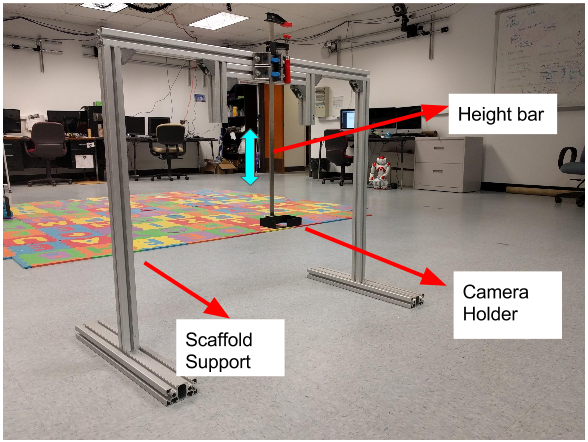
\includegraphics[width=\textwidth]{imaging_rig_labeled}
      \caption{}
      \label{fig:im_rig_side}
  \end{subfigure}
  \begin{subfigure}[]{0.45\textwidth}
      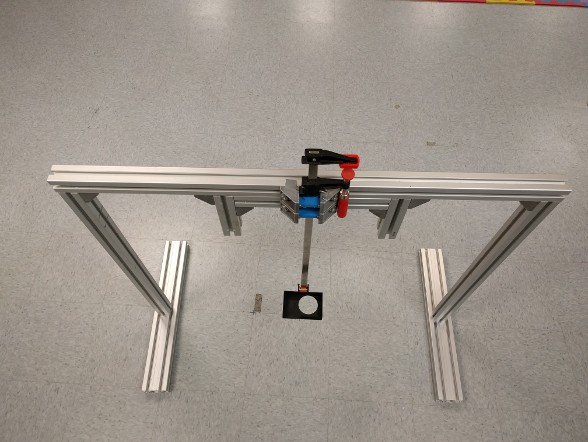
\includegraphics[width=\textwidth]{imaging_rig_top_scaled}
      \caption{}
      \label{fig:im_rig_top}
  \end{subfigure}
\caption[Imaging rig used for data collection in multi-image object recognition approach]{The imaging rig allows the height bar to slide up or down, thereby letting the height of the camera from the ground to be varied. The different components of the imaging rig are labeled in (\subref{fig:im_rig_side}). The camera holder attached to the lower end of the height bar is designed to carry a GoPro Hero 4 camera.}
\label{fig:im_rig}
\end{figure*}	

%======================================================================================================
\subsubsection{Imaging Environment}


\begin{enumerate}
	\item Since underwater object recognition could pose a challenging problem due to presence of noise and lighting variations, data was collected in a test tank filled with water.
\end{enumerate}


The environment where object recognition experiments are performed could affect the performance of the algorithm used. In case of an environment with limited to no control over the imaging parameters, the level of noise introduced into the sensor measurements is difficult to gauge. This complicates the task of designing noise filters to take any corrective measures. It might be tempting to perform object recognition experiments in controlled laboratory conditions, thereby allowing the possibility to tune the environmental parameters to enhance the performance of an algorithm. However, if an algorithm is intended to operate on natural images, there are often going to be unpredictable variations in environmental factors that could adversely affect the performance of the algorithm. To accurately validate an algorithm that is intended to operate on natural environments, it is imperative to choose a 
test environment where the conditions are close to the expected natural conditions. Following this line of reasoning, since this object recognition algorithm is intended to operate on noisy natural environments, an underwater environment with uncontrolled lighting was chosen as the test environment. A circular tank in the Robot Discovery Lab (RDL) at University of Delaware filled with 4 feet of fresh water was thus utilized to collect experimental data. The imaging rig described in Section~\ref{sec:imaging_rig} was submerged inside this test tank during the data collection process.

%======================================================================================================
\subsubsection{Object Specimens}


\begin{enumerate}
	\item To validate the developed multi-image recognition method, commonly available produce like orange and strawberry were selected as they offered specimens with natural intra-class along with significant inter-class differences in appearance.
\end{enumerate}


The focus of this work is to recognize a class of objects that can exhibit some level of intra-class variance that is characteristic to naturally occurring objects. One such example is underwater marine organisms, where each species can have several identifiers that distinguish them from a different species. However in most cases, the members of a single species also exhibit some level of variation in their appearance. To accommodate such cases, the specimens used to validate this multi-view object recognition algorithm were required to have \begin{enumerate*}[label=(\roman*)]  \item some characteristics that are unique to the class they belong to \item small variations with regards to appearance within the same class of objects, and \item easy accessibility for experimentation purposes. \end{enumerate*} All these points were satisfied by natural produce like potatoes, oranges, tomatillos and strawberries. Natural produce exhibit significant inter-class variance, sufficient intra-class variance and are 
readily 
available in stores making them ideal 
candidates for object specimens. Figure~\ref{fig:produce_species} shows an assortment of potatoes and tomatillos to visually reinforce the inter-class and intra-class variance exhibited by naturally occurring objects. The underwater data on which this multi-view algorithm is validated is composed of a set of 11 oranges and 11 strawberries.
%
\begin{figure*}
  \centering
  \begin{subfigure}[]{0.45\textwidth}
      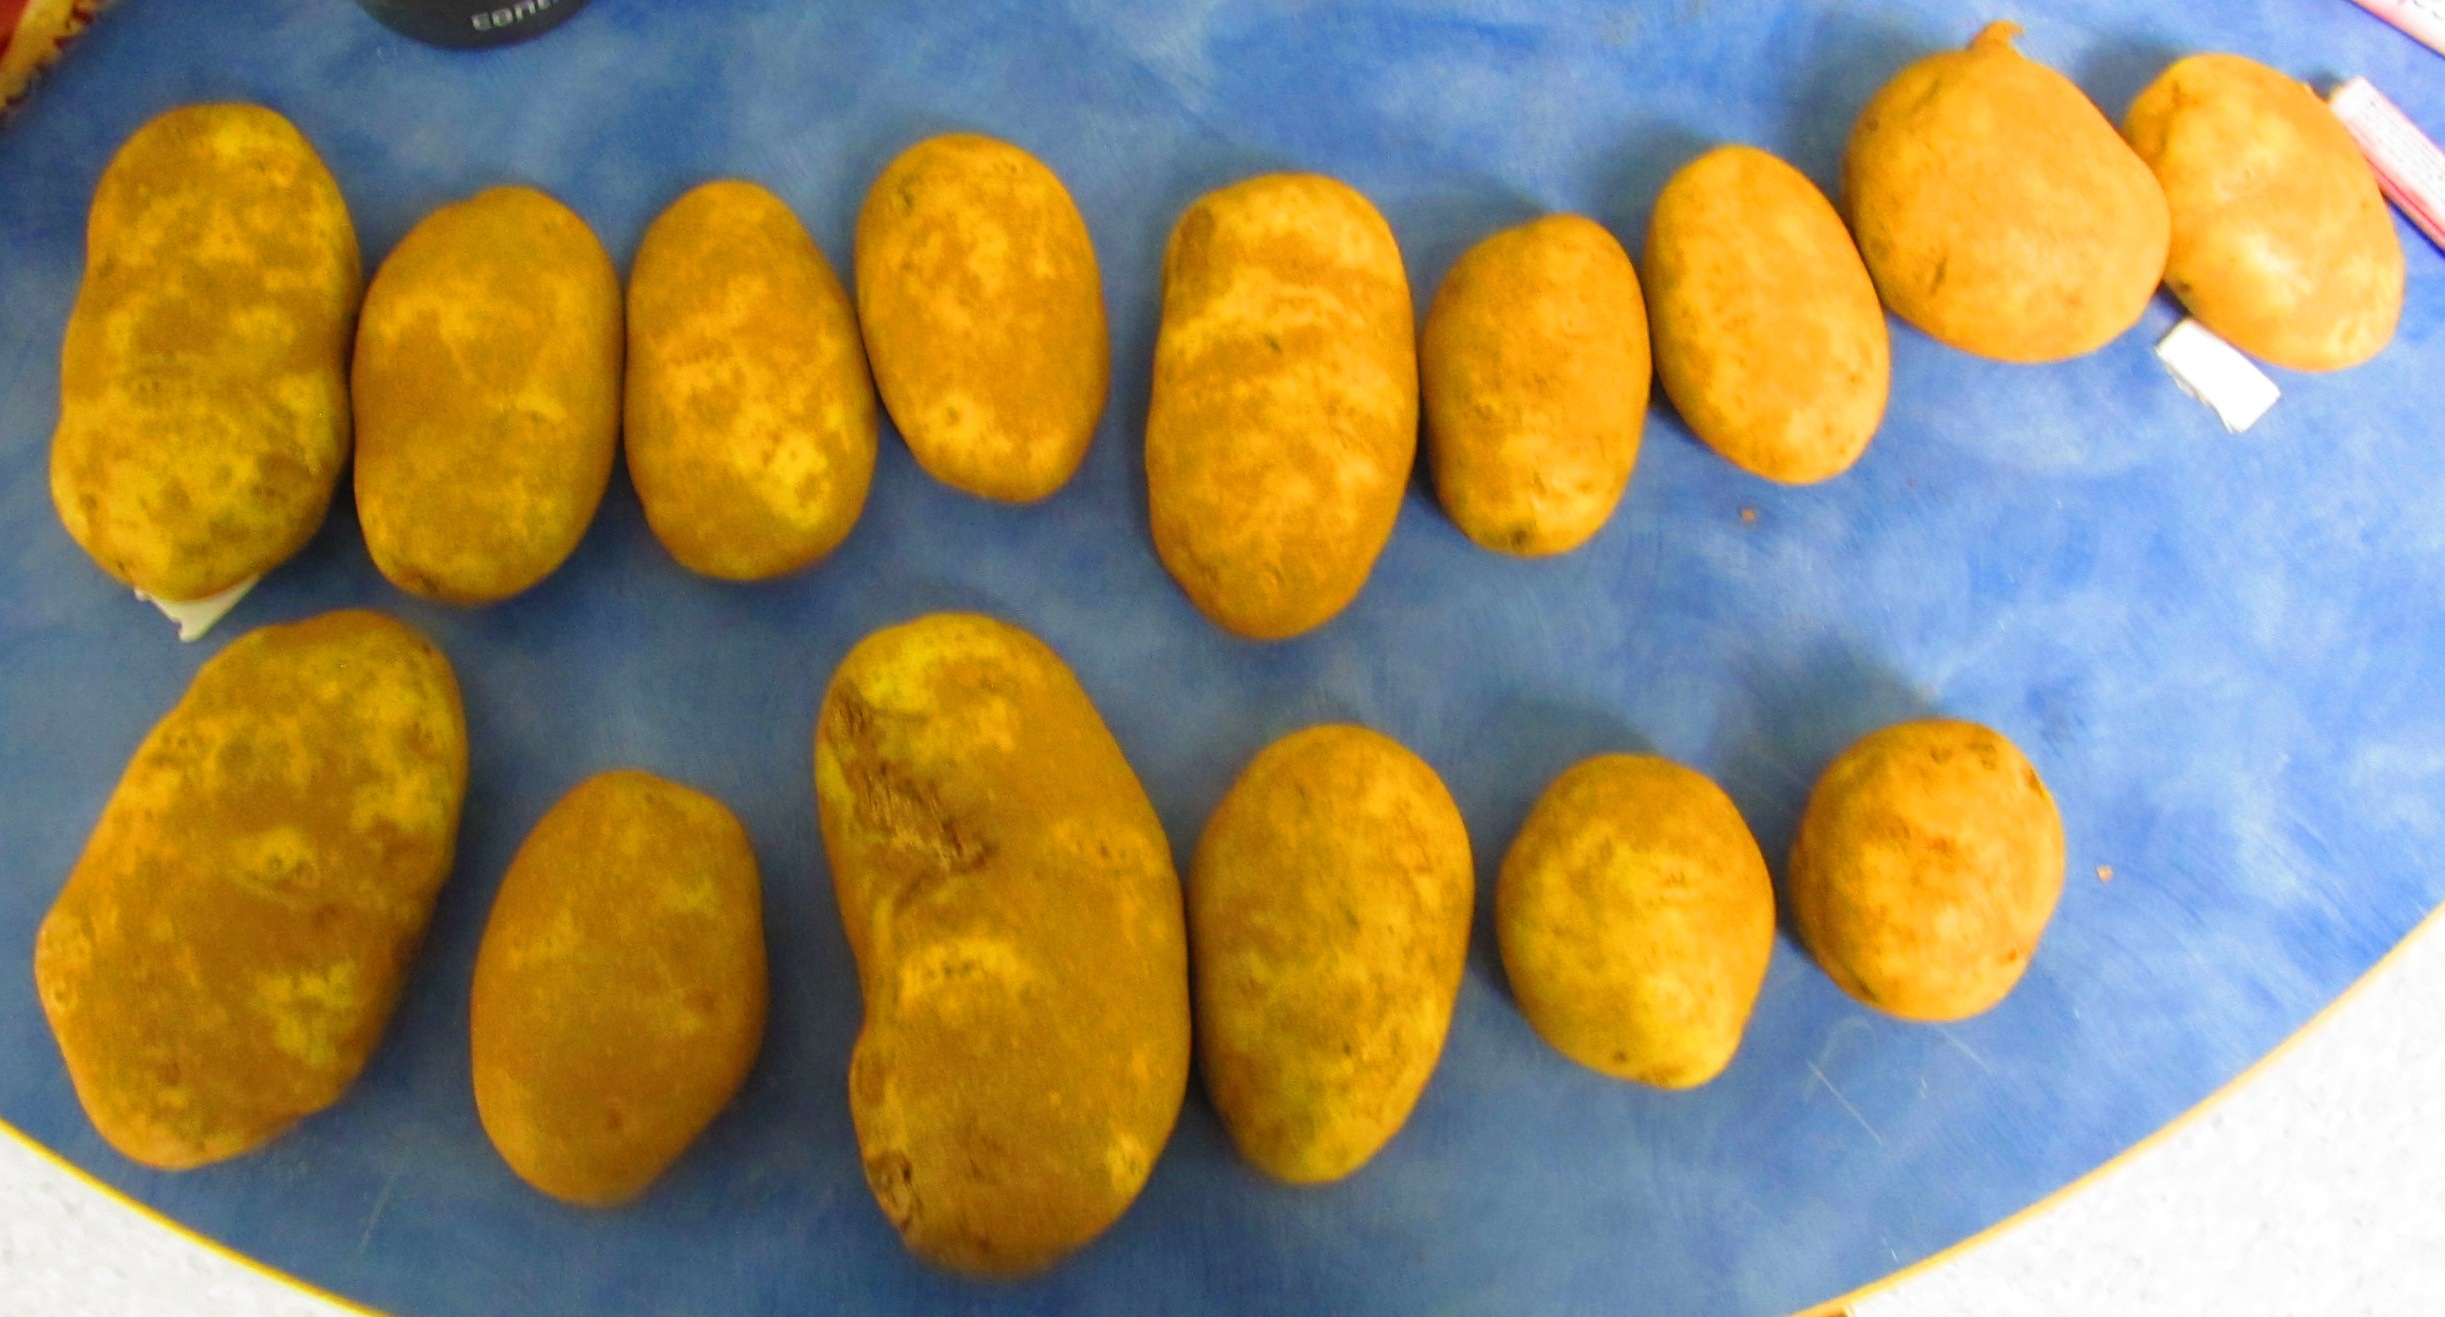
\includegraphics[width=\textwidth]{potatoes_species}
      \caption{Potatoes}
      \label{fig:potato_species}
  \end{subfigure}
  \begin{subfigure}[]{0.45\textwidth}
      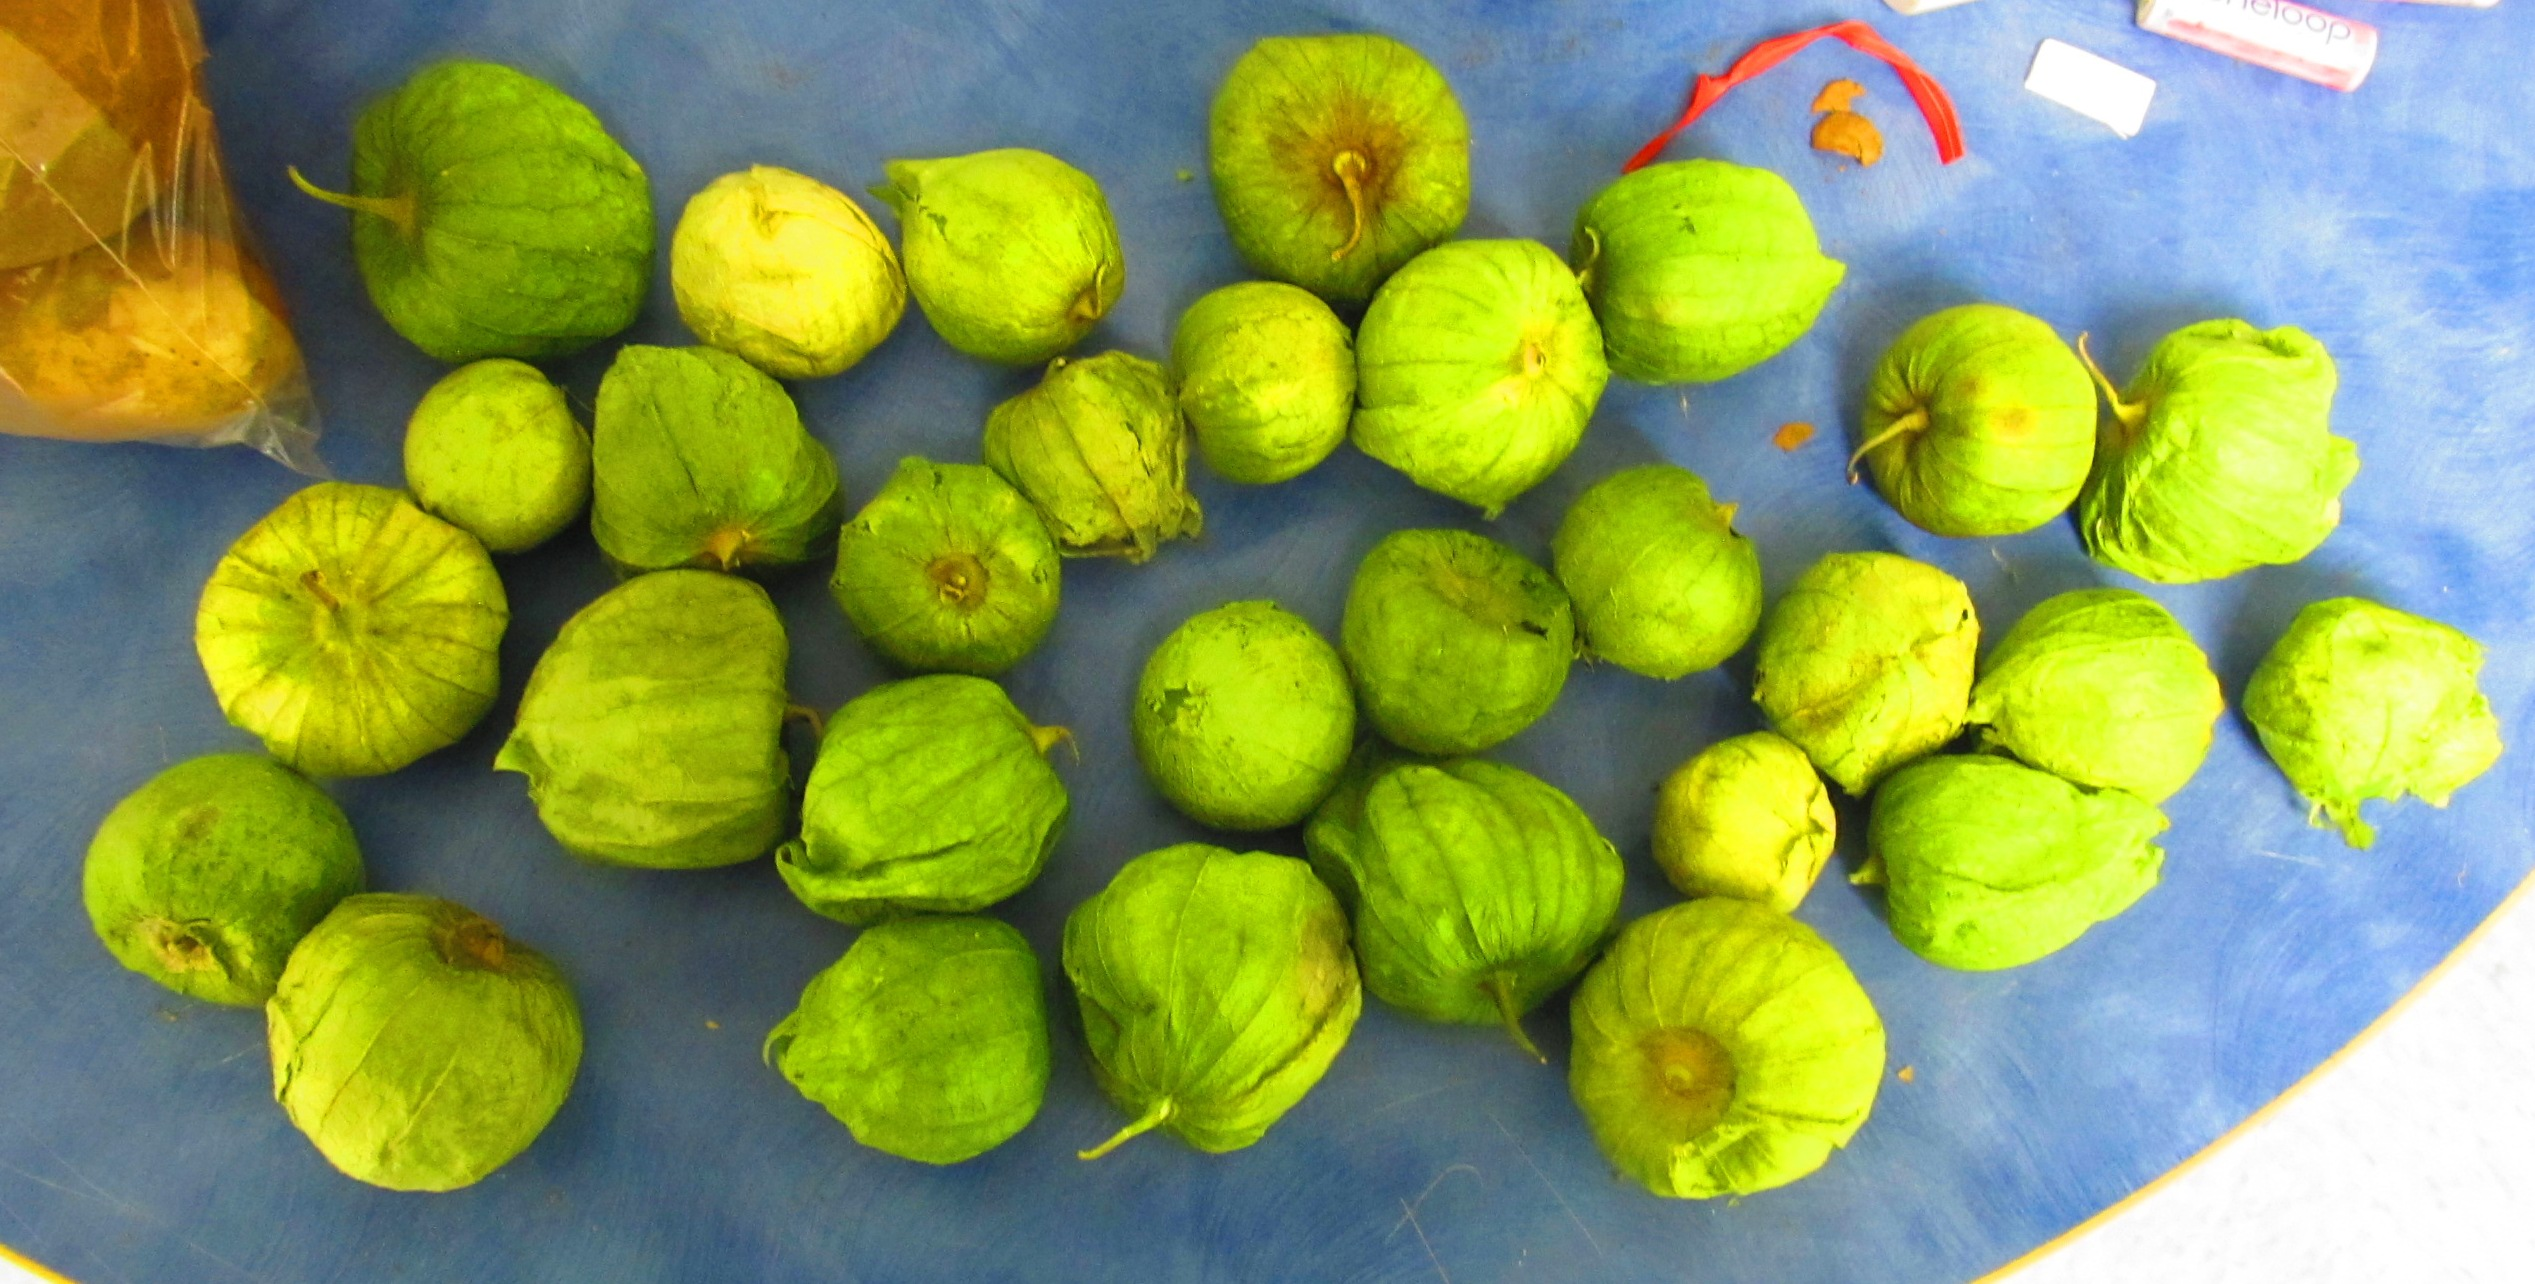
\includegraphics[width=\textwidth]{tomatillos_species}
      \caption{Tomatillos}
      \label{fig:tomatillo_species}
  \end{subfigure}
\caption[Illustration of the inter-class and intra-class variance exhibited by naturally occurring objects]
{An illustration of the inter-class and intra-class variance exhibited by naturally occurring objects like 
potatoes (\subref{fig:potato_species}) and tomatillos (\subref{fig:tomatillo_species})}.
\label{fig:produce_species}
\end{figure*}	
%
%================================================================================================================
\section{Definitions}

\subsection{Histogram Signature}
\label{sec:hist_signature}

As a part of this object recognition technique we define a histogram signature that improves on the generic histogram, specifically designed to deal with possible noise in the pixel values. The rest of this section defines this histogram signature.

A generic histogram $H_f:b_i\mapsto n_i$ of some colorspace $f$, captures the distribution of values of pixels in colorspace $f$, where $n_i$ represents the count of bin $b_i \in \mathcal{B}$, and $\mathcal{B}$ is the set of bins used to partition colorspace $f$. Any pixels affected by noise in image $I$ could corrupt the histogram $H_f$. If we assume that $e\%$ of the pixel values of an image constitutes noise, then the histogram $H_f$ can be refined by rejecting bins containing $e\%$ of pixel values that are least likely to occur according to histogram $H_f$. Before computing the refined version of this histogram, the histogram $H_f$ is first normalized into the form $\bar{H}_f:b_i\mapsto \bar{n}_i$ where
%
\begin{align}	\label{eqn:hist_norm}
 \bar{H}_f(b_i)=\frac{n_i}{\sum_{j}n_j}=\bar{n}_i \enspace.
\end{align}
Now the refined \emph{histogram signature} $\mathcal{H}_f:b_i\mapsto n'_i$ is computed, such that
\begin{align}
  n'_i = 
  \begin{cases}
     \bar{n}_i & b_i \in \bar{\mathcal{B}}_e\\
     0	&	b_i \in \mathcal{B}_e
  \end{cases},
\end{align}
%
where $\mathcal{B}_e$ and $\bar{\mathcal{B}}_e$ constitute a binary partition of $\mathcal{B}$, 
i.e. $\mathcal{B}_e \cap \bar{\mathcal{B}}_e = \phi \text{ and } 
\mathcal{B}_e \cup \bar{\mathcal{B}}_e = \mathcal{B}$,
chosen in a way that 
$\bar{\mathcal{B}}_e$ is the smallest cardinality subset of 
$\mathcal{B}$ that satisfies the condition $\sum_{b_i \in \bar{\mathcal{B}}_e} \bar{H}_f(b_i) > 1-e$. 
The definition of set $\bar{\mathcal{B}}_e\subseteq\mathcal{B}$ can be restated as
\begin{align}
 \bar{\mathcal{B}}_e=\underset{|\bar{\mathcal{B}_e}|} {\mathrm{argmin}} \sum_{b_i \in \bar{\mathcal{B}_e}} \bar{H}_f(b_i) > 1-e
\end{align}

The $|\mathcal{B}|$-element histogram signature $\mathcal{H}_f$ now encodes the histogram information while attempting to filter some of the noise present in sensor measurements.

\section{Methodology}
\label{sec:distdes_methodology}

\begin{enumerate}
	\item Any machine learning technique like the one used here for object recognition comprises a learning and a testing phase.
	
	\item The learning phase of object recognition involves extracting features that are capable of identifying a target unambiguously.
	
	\item The testing phase is the application of the learned machine learning model to an application where the identity of an object is to be ascertained.
	
	\item To validate the developed theory, an image dataset with images of objects captured from different known heights was gathered.
\end{enumerate}	


The distance-based global descriptor algorithm presented in this chapter is essentially a machine learning technique. As it is common with such techniques, it consists of two parts: a learning part and a validation part. In the learning phase, features and other attributes of an object class are captured from labeled instances of the object available in the learning set. In the validation phase, the learned descriptor for an object class is validated against pre-labeled images to evaluate the performance of an algorithm. The data collection and annotation phases that provide data used for learning and validation parts of this algorithm are discussed next.

\subsection{Data Collection}
\label{sec:distdes_data_collection}

\begin{enumerate}
  \item 13 Images of each target is captured between heights of 32in and 8in with an interval of 2in.
\end{enumerate}	


The data collection process here involves capturing 13 images for each object specimen. For the validation of this multi-view object recognition algorithm, data was gathered from 22 specimens (11 oranges and 11 strawberries) bringing the total images collected to $286\, (22\enspace \text{specimens} \times 13\enspace \text{images per specimen})$. Each specimen was first placed on the floor below the camera-holder on the imaging rig (see Figure~\ref{fig:im_rig}). The height bar was moved up till the camera holder was $32$ inches away from the ground. A GoPro Hero 4 camera, attached to the holder, was then triggered to capture an image of the specimen. This first image captured the visual appearance of the specimen 32 inches away from the ground. After the first image was captured and without disturbing the object, the next image was captured after lowering the height bar such that the camera was now $30$ inches away from the ground.
This process of lowering the camera by 2 inches between subsequent images is continued till the camera gets to a height of $8$ inches away from the ground. 
The series of images captured from a range of heights, from 32 inches to 8 inches, every 2 inches results in 13 images per specimen. 
These 13 images capture the appearance of a specimen at different heights. An illustration of the 13 images captured for a strawberry and orange specimen is shown in Figure~\ref{fig:height_specimen}. An important point to note here is that the imaging rig is handled manually between each image capture which sometimes results in displacement of the imaging rig or the specimen. 
Additional disturbances in the underwater testing environment where the specimen was placed, added another source of inconsistency that sometimes lead to the specimen or the imaging rig getting displaced during the data collection process. These uncontrolled factors in the data collection process added some level of variance to the gathered dataset.
Since this algorithm is intended to operate on uncontrolled natural environments, such variance in the collected data was welcomed to some degree, given that it could test the algorithm's robustness.

\begin{figure*}
  \centering
  \begin{subfigure}[]{\textwidth}
      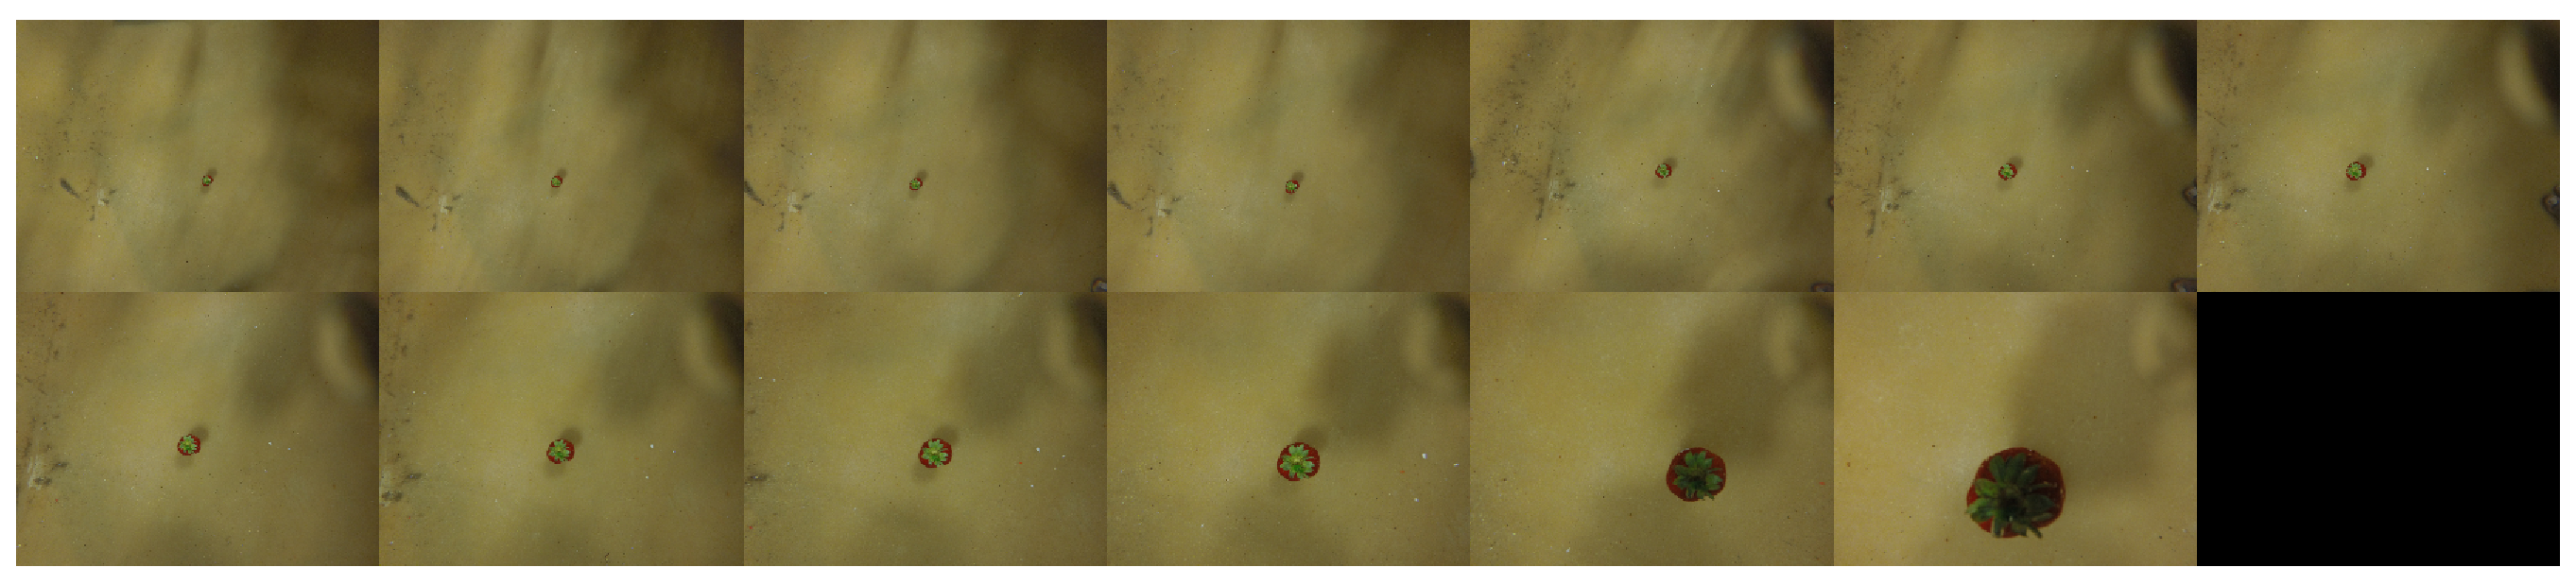
\includegraphics[width=\textwidth]{strawberry_distance_montage.eps}
      \caption{Strawberry specimen seen from different heights}
      \label{fig:strawberry_height_specimen}
  \end{subfigure}
  \begin{subfigure}[]{\textwidth}
      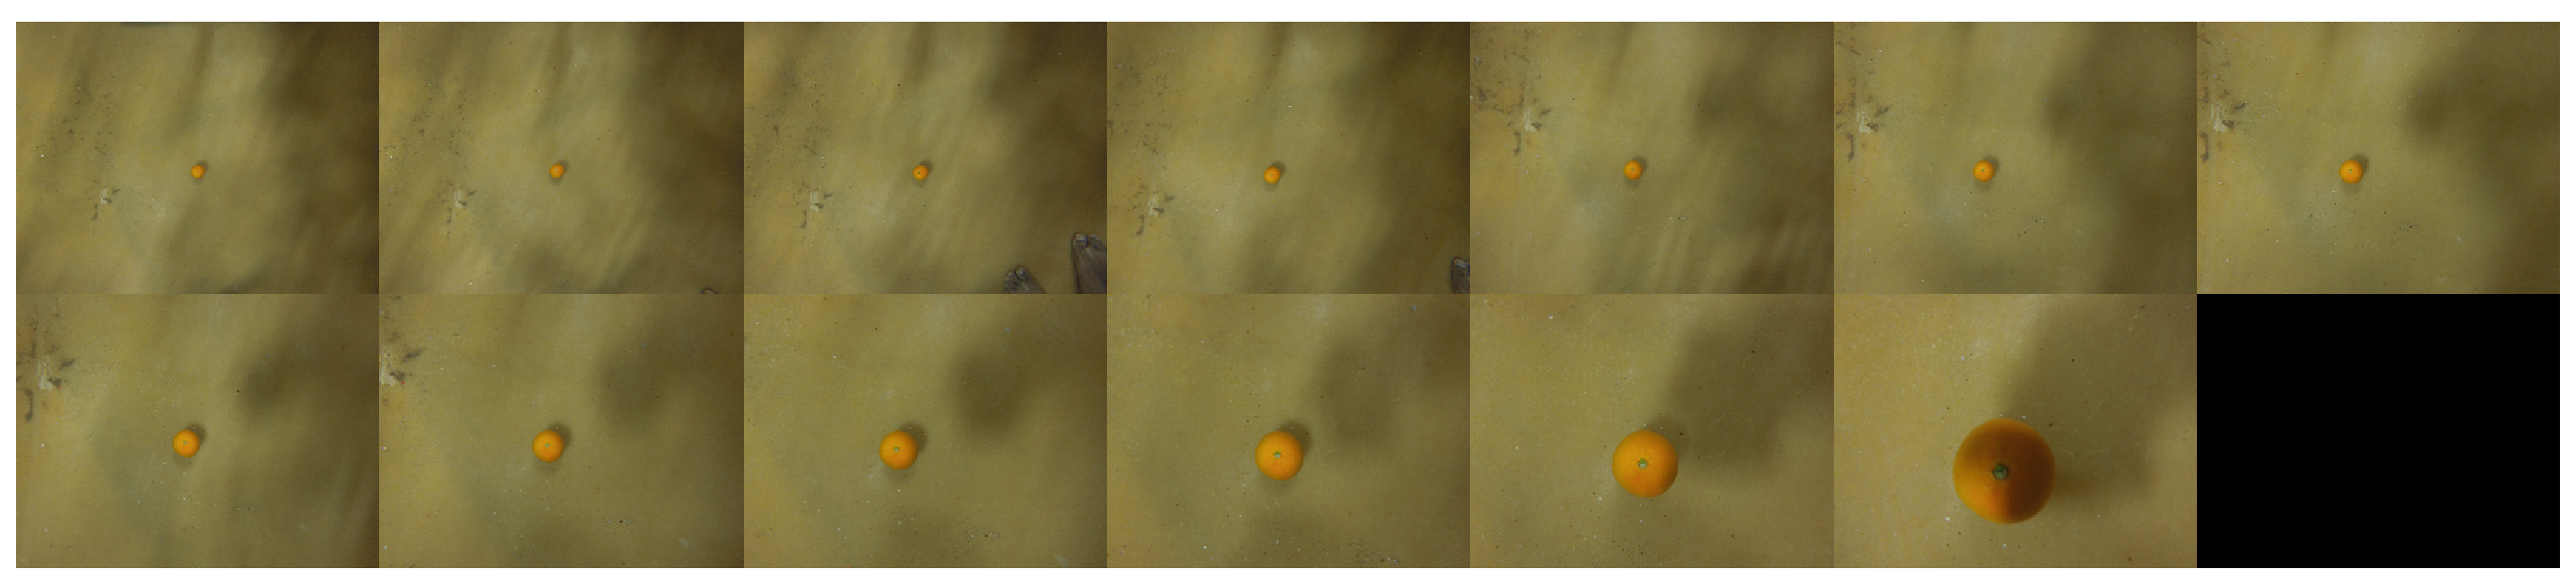
\includegraphics[width=\textwidth]{orange_distance_montage.eps}
      \caption{Orange specimen seen from different heights}
      \label{fig:orange_height_specimen}
  \end{subfigure}
\caption[Set of images collected for each specimen from different heights]{A set of 13 images gathered for a specimen (strawberry in (\subref{fig:strawberry_height_specimen}) and orange in (\subref{fig:orange_height_specimen})) starting from a height of 32 inches (top left) up to a height of 8 inches (bottom right) away from the target.
Each subsequent image was captured 2 inches closer to the specimen.}
\label{fig:height_specimen}
\end{figure*}	
%
Due to the wide-angle fish-eye lens of the GoPro camera used, the ratio of the pixels of the object specimen to the background could be very small when the camera is far away from the target. In technical terms, when the images of a target are captured by a camera that is far away from a specimen, the number of pixels that correspond to the specimen in a image could be statistically insignificant. This reported object recognition procedure depends on histograms of images (more details of how the histogram is relevant is explained in Section~\ref{sec:distdes_methodology}). 
For the histogram to accurately capture the properties of a specimen, the images of the specimen need to have a relatively high ratio of object pixels over background pixels. To improve this ratio of object pixels in the image, the images were cropped to discard a portion of background. The strawberry and orange specimens shown in Figure~\ref{fig:strawberry_height_specimen} and Figure~\ref{fig:orange_height_specimen} are shown again in Figure~\ref{fig:strawberry_height_specimen_cropped} and 
Figure~\ref{fig:orange_height_specimen_cropped} respectively, after cropping of portions of background.

\begin{figure*}
  \centering
  \begin{subfigure}[]{0.12\textwidth}
      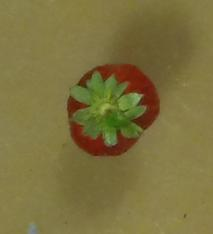
\includegraphics[width=\textwidth]{strawberry4_obj_01/strawberry4_001_32}
      \caption{}
  \end{subfigure}
  \begin{subfigure}[]{0.12\textwidth}
      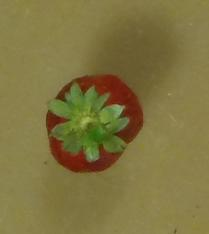
\includegraphics[width=\textwidth]{strawberry4_obj_01/strawberry4_001_30}
      \caption{}
  \end{subfigure}
  \begin{subfigure}[]{0.12\textwidth}
      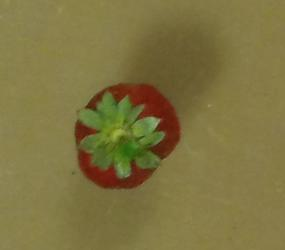
\includegraphics[width=\textwidth]{strawberry4_obj_01/strawberry4_001_28}
      \caption{}
  \end{subfigure}
  \begin{subfigure}[]{0.12\textwidth}
      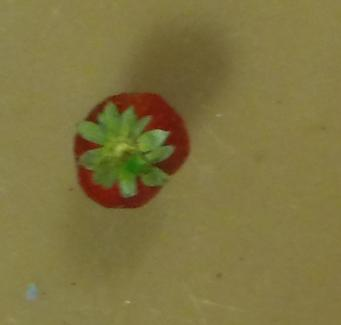
\includegraphics[width=\textwidth]{strawberry4_obj_01/strawberry4_001_26}
      \caption{}
  \end{subfigure}
  \begin{subfigure}[]{0.12\textwidth}
      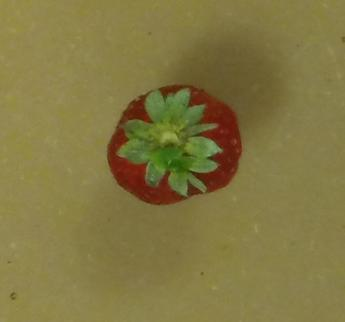
\includegraphics[width=\textwidth]{strawberry4_obj_01/strawberry4_001_24}
      \caption{}
  \end{subfigure}
  \begin{subfigure}[]{0.12\textwidth}
      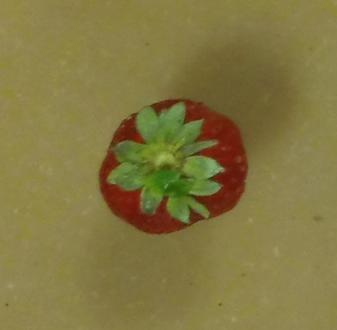
\includegraphics[width=\textwidth]{strawberry4_obj_01/strawberry4_001_22}
      \caption{}
  \end{subfigure}
  \begin{subfigure}[]{0.12\textwidth}
      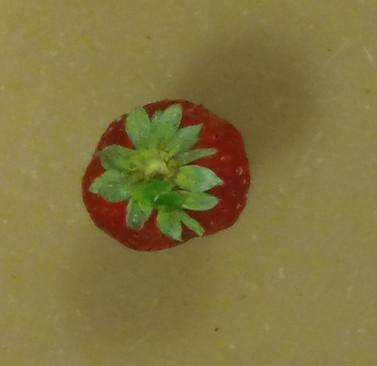
\includegraphics[width=\textwidth]{strawberry4_obj_01/strawberry4_001_20}
      \caption{}
  \end{subfigure}
  \begin{subfigure}[]{0.12\textwidth}
      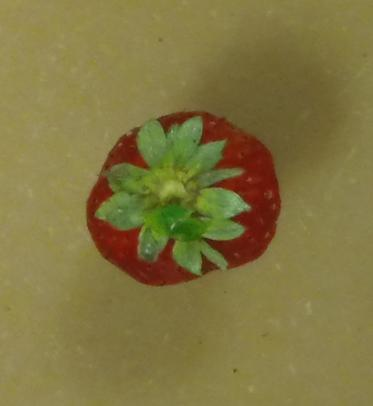
\includegraphics[width=\textwidth]{strawberry4_obj_01/strawberry4_001_18}
      \caption{}
  \end{subfigure}
  \begin{subfigure}[]{0.12\textwidth}
      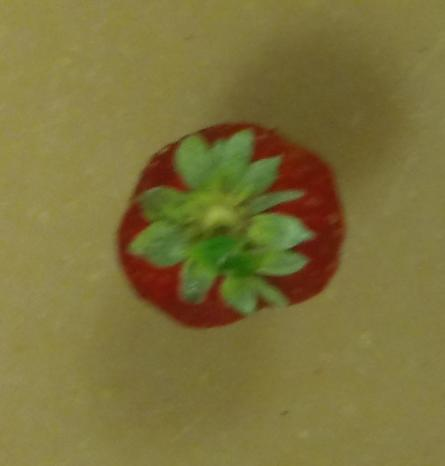
\includegraphics[width=\textwidth]{strawberry4_obj_01/strawberry4_001_16}
      \caption{}
  \end{subfigure}
  \begin{subfigure}[]{0.12\textwidth}
      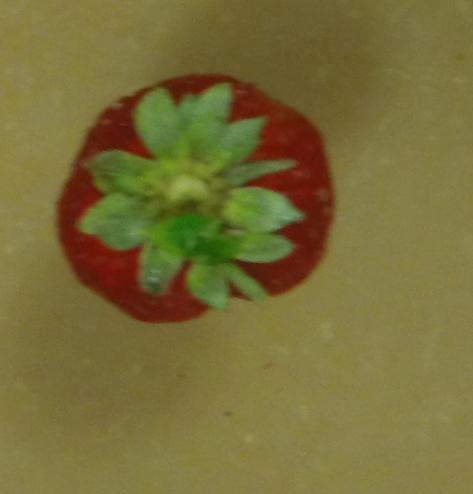
\includegraphics[width=\textwidth]{strawberry4_obj_01/strawberry4_001_14}
      \caption{}
  \end{subfigure}
  \begin{subfigure}[]{0.12\textwidth}
      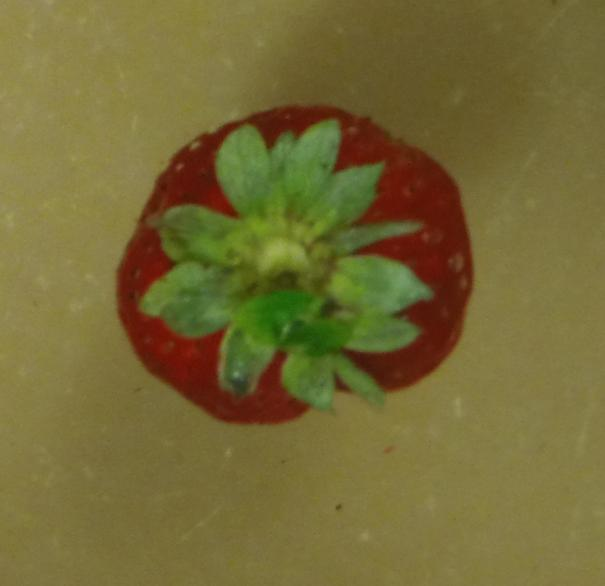
\includegraphics[width=\textwidth]{strawberry4_obj_01/strawberry4_001_12}
      \caption{}
  \end{subfigure}
  \begin{subfigure}[]{0.12\textwidth}
      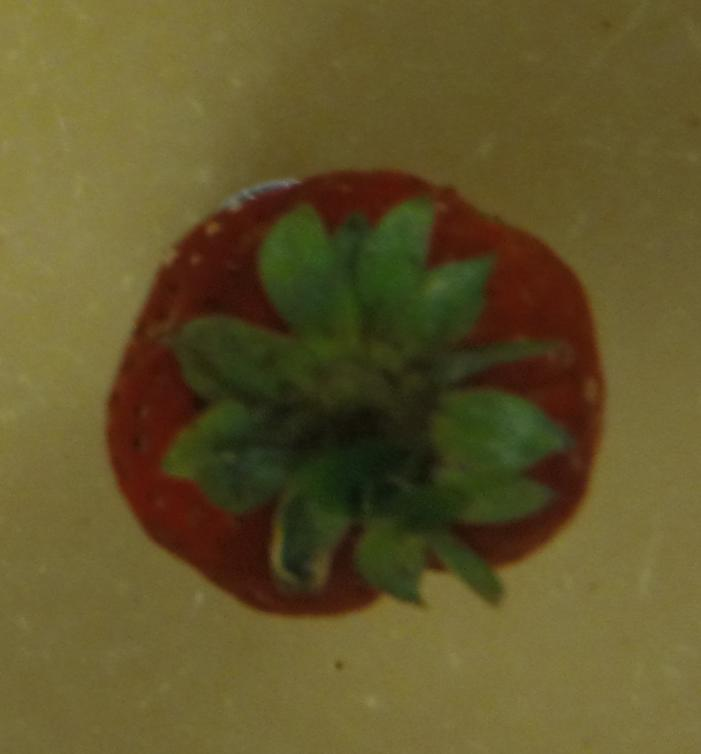
\includegraphics[width=\textwidth]{strawberry4_obj_01/strawberry4_001_10}
      \caption{}
  \end{subfigure}
  \begin{subfigure}[]{0.12\textwidth}
      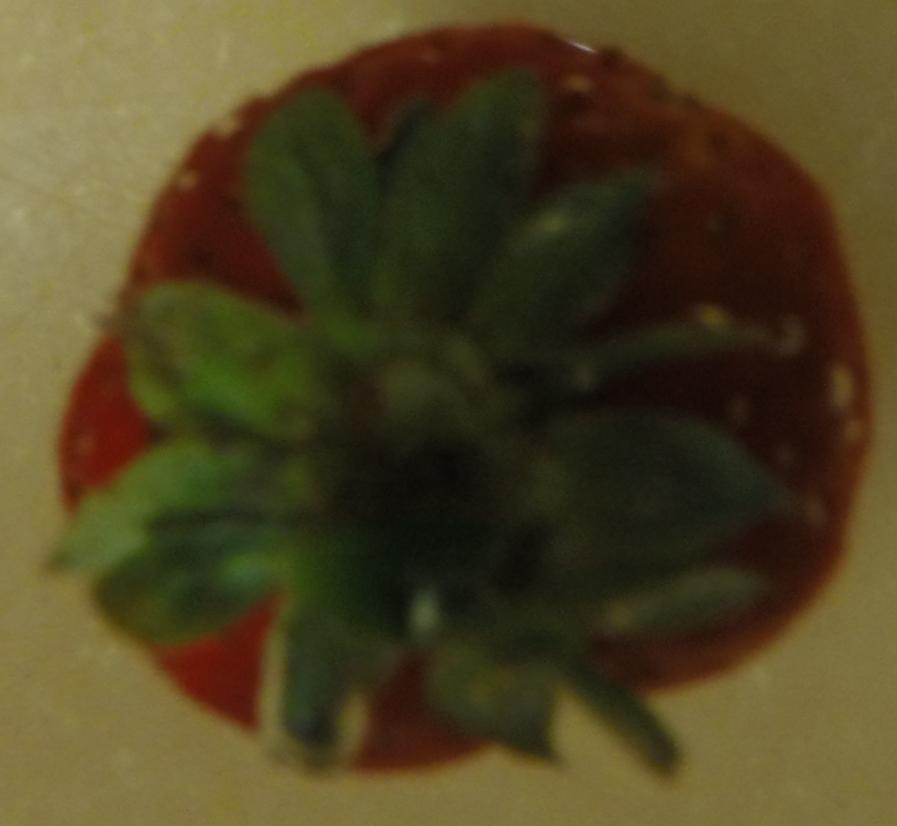
\includegraphics[width=\textwidth]{strawberry4_obj_01/strawberry4_001_08}
      \caption{}
  \end{subfigure}
\caption[Images of a strawberry specimen after cropping a portion of background]{The strawberry specimen in Figure~\ref{fig:strawberry_height_specimen} shown after cropping a portion of the background}
\label{fig:strawberry_height_specimen_cropped}
\end{figure*}	

\begin{figure*}
  \centering
  \begin{subfigure}[]{0.12\textwidth}
      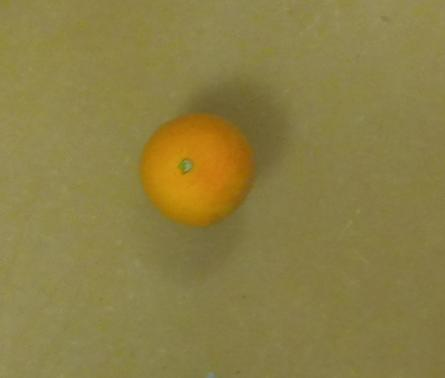
\includegraphics[width=\textwidth]{orange4_obj_11/orange4_011_32}
      \caption{}
  \end{subfigure}
  \begin{subfigure}[]{0.12\textwidth}
      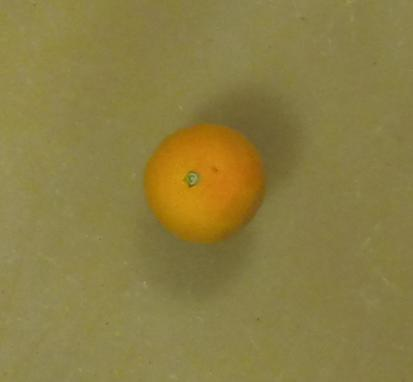
\includegraphics[width=\textwidth]{orange4_obj_11/orange4_011_30}
      \caption{}
  \end{subfigure}
  \begin{subfigure}[]{0.12\textwidth}
      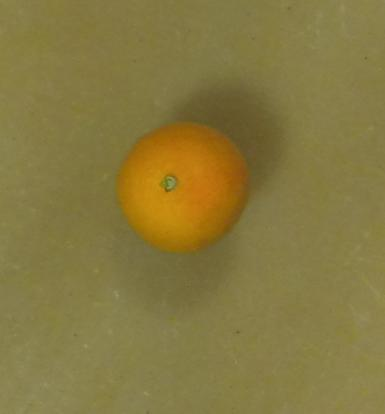
\includegraphics[width=\textwidth]{orange4_obj_11/orange4_011_28}
      \caption{}
  \end{subfigure}
  \begin{subfigure}[]{0.12\textwidth}
      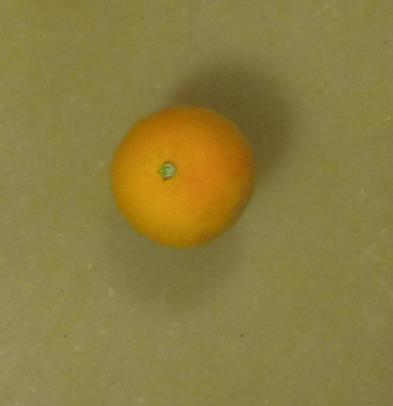
\includegraphics[width=\textwidth]{orange4_obj_11/orange4_011_26}
      \caption{}
  \end{subfigure}
  \begin{subfigure}[]{0.12\textwidth}
      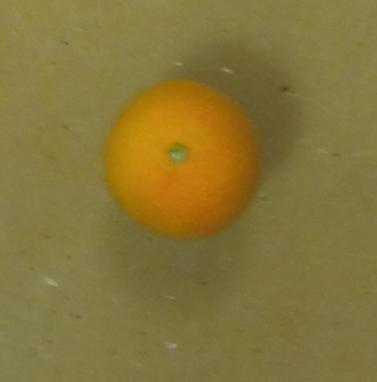
\includegraphics[width=\textwidth]{orange4_obj_11/orange4_011_24}
      \caption{}
  \end{subfigure}
  \begin{subfigure}[]{0.12\textwidth}
      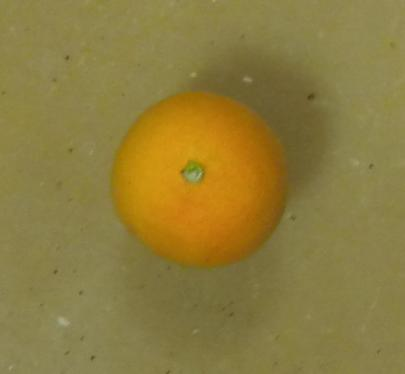
\includegraphics[width=\textwidth]{orange4_obj_11/orange4_011_22}
      \caption{}
  \end{subfigure}
  \begin{subfigure}[]{0.12\textwidth}
      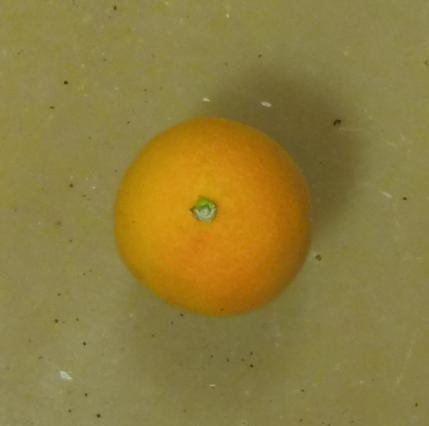
\includegraphics[width=\textwidth]{orange4_obj_11/orange4_011_20}
      \caption{}
  \end{subfigure}
  \begin{subfigure}[]{0.12\textwidth}
      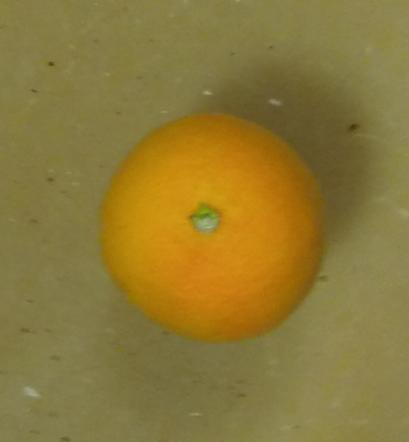
\includegraphics[width=\textwidth]{orange4_obj_11/orange4_011_18}
      \caption{}
  \end{subfigure}
  \begin{subfigure}[]{0.12\textwidth}
      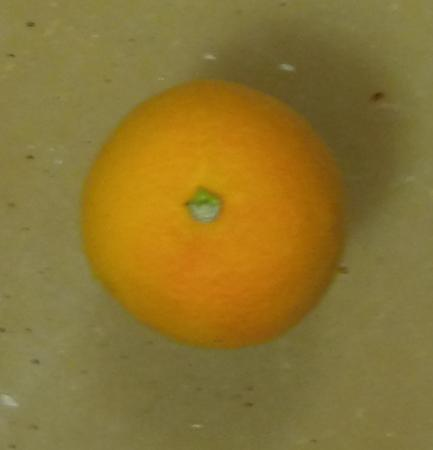
\includegraphics[width=\textwidth]{orange4_obj_11/orange4_011_16}
      \caption{}
  \end{subfigure}
  \begin{subfigure}[]{0.12\textwidth}
      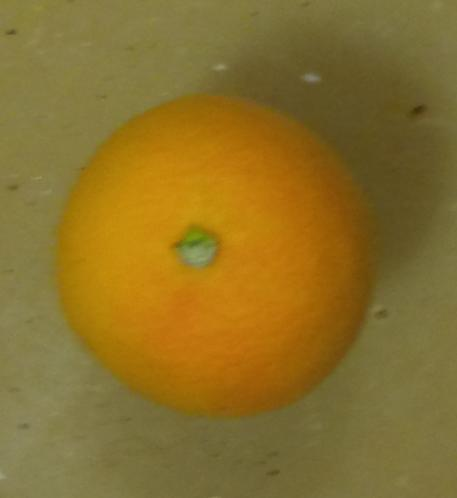
\includegraphics[width=\textwidth]{orange4_obj_11/orange4_011_14}
      \caption{}
  \end{subfigure}
  \begin{subfigure}[]{0.12\textwidth}
      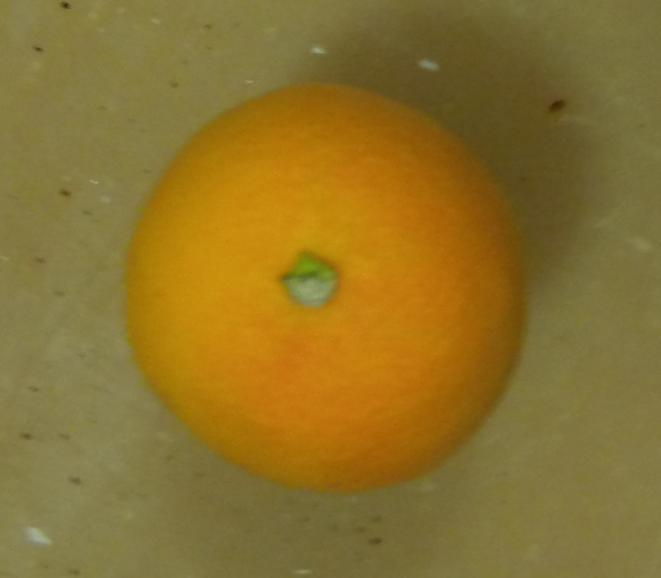
\includegraphics[width=\textwidth]{orange4_obj_11/orange4_011_12}
      \caption{}
  \end{subfigure}
  \begin{subfigure}[]{0.12\textwidth}
      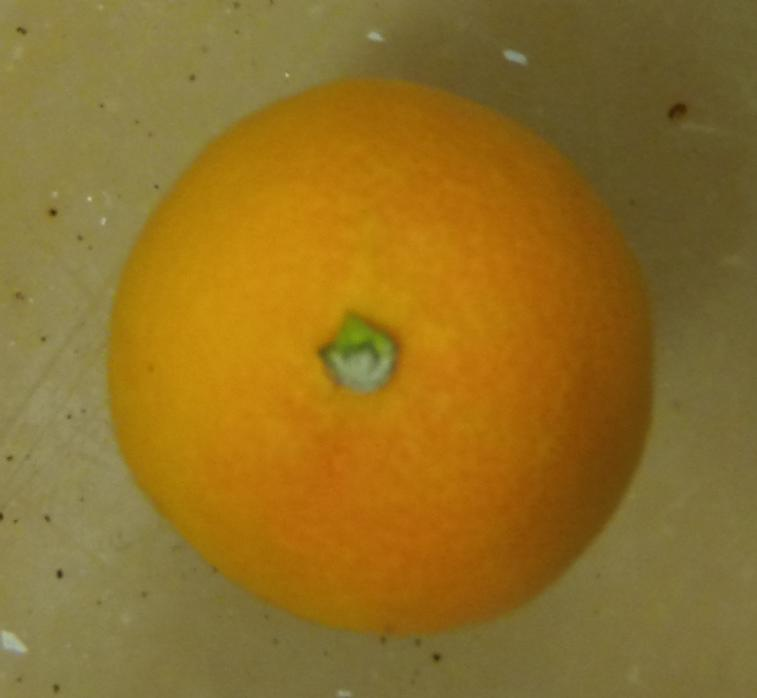
\includegraphics[width=\textwidth]{orange4_obj_11/orange4_011_10}
      \caption{}
  \end{subfigure}
  \begin{subfigure}[]{0.12\textwidth}
      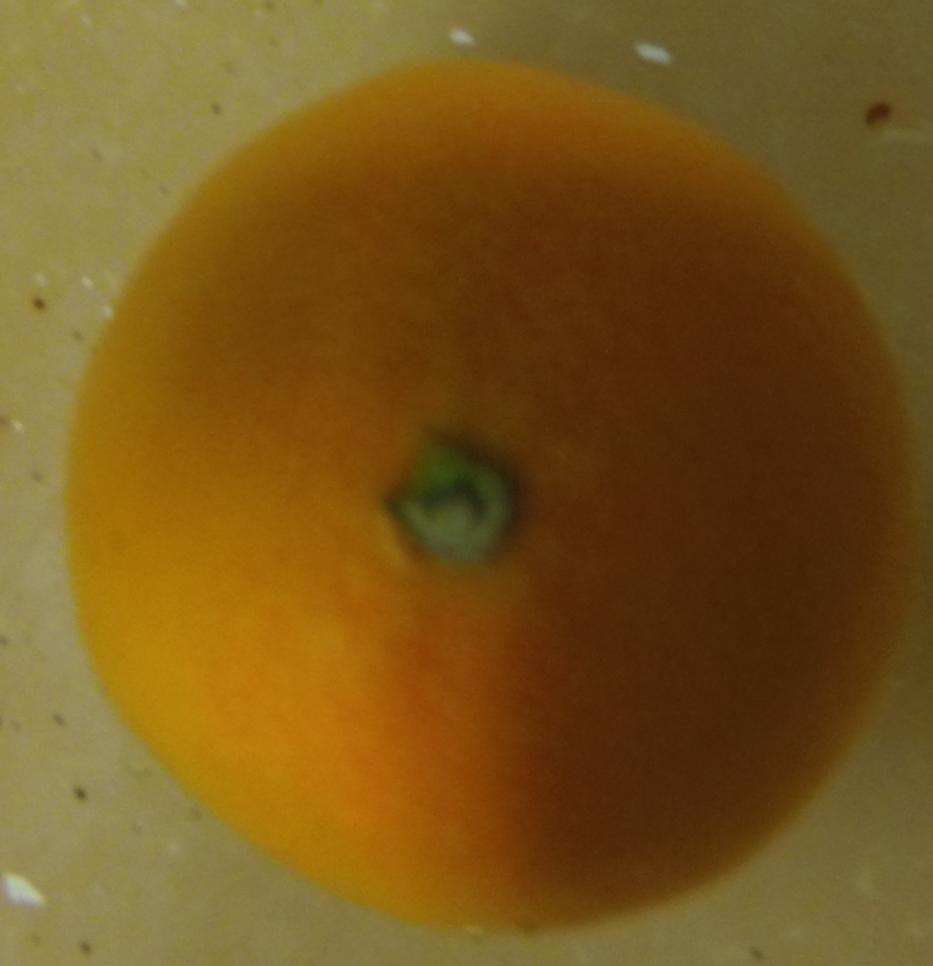
\includegraphics[width=\textwidth]{orange4_obj_11/orange4_011_08}
      \caption{}
  \end{subfigure}
\caption[Images of an orange specimen after cropping a portion of background]{The orange specimen in Figure~\ref{fig:orange_height_specimen} shown after cropping a portion of the background}
\label{fig:orange_height_specimen_cropped}
\end{figure*}	


\subsection{Annotation Process}
\label{sec:distdes_annotation}

The task of manual image annotation is a costly and labor intensive process. Developing an object recognition algorithm is often motivated by a desire to avoid manual inspection in order to identify objects from images. However, to build a machine learning framework for object recognition, an initial set of images needs to be annotated manually to contribute to the learning set. 
Just like any other supervised machine learning algorithm, this procedure requires annotation of images into labeled foreground and background. Here, each learning sample consists of 13 images of a specimen captured from different heights. Increasing the number of images of each specimen quickly increases the annotation load. To mitigate this burden, a semi-automated annotation framework is developed.

In the first stage of the annotation process, a customized \gls{buva} technique (described in Section~\ref{sec:visual_attn}) is used to pick the most \textit{interesting} point in an image. This most \textit{interesting} point is referred to as the first fixation. According to the visual attention hypothesis, if a distribution of features can be used to characterize an image, the first fixation corresponds to the point in the image which is most unlikely to belong to this distribution of features. In other words, the first fixation corresponds to a point that does not belong to the background and hence most likely is a foreground object pixel. In the first stage of this semi-automated annotation process, the first fixation point along with all its neighboring pixels are assumed to be foreground pixels. Thus a rectangle of dimensions $15\%$ image width $\times 15\%$ image height, centered on the fixation is assumed to be the foreground region. We will refer to this rectangle as the \textit{foreground 
hypothesis rectangle}.
Since the data collection  process ensures that an object in an image is close to the center of the image rather than the edge, the pixels in the boundary of the images can safely be assumed to be background pixels. Hence, rectangular blocks of pixels in the 4 corners of an image are assumed to be background pixels. Each of these background blocks is $5\%$ image width $\times 5\%$ image height in dimension. This foreground and background pixel hypothesis is used in the next stage of the annotation process to segment the image into foreground and background. A visual representation of the background and foreground seed pixels is shown in Figure~\ref{fig:good_seg_visualattn_seeds} as blue and red rectangles, respectively. The visual attention fixation is shown here as a green dot.

The foreground and background seeds thus obtained can be used to initialize a grabcut-in-one-cut algorithm \cite{onecut}. This grabcut-in-one-cut algorithm, a variant of graphcut algorithm (described in Section~\ref{sec:onecut}) splits an input image into background and foreground. Grabcut-in-one-cut algorithm operates by labeling pixels \textit{similar} in appearance to foreground seeds as foreground and the other pixels that appear closer to background seeds as background.
However, the foreground seeds supplied by visual attention, might not produce accurate results in all cases. There are often instances when the fixation tagged as foreground constitutes edge pixels of an object. Since object edge pixels of an object are essentially discontinuities indicating a transition between foreground and background pixel distributions, the likelihood of visual attention picking edge pixels as fixations is high. If an object edge pixel is picked as the first fixation, this could result in foreground hypothesis rectangle, erroneously containing background pixels. An illustration of this effect can be seen in Figure~\ref{fig:good_seg_visualattn_seeds} where the green dot at the edge of the object is the visual attention fixation. The blue foreground hypothesis rectangle around the fixation point contains some wrongly labeled background pixels. Wrongly labeled background pixels in foreground seeds supplied to graphcut algorithm can result in inaccurate segmentation, as in the case seen in 
Figure~\ref{fig:good_seg_visualattn_seg}. Thus, to improve the performance of the graphcut algorithm, we use a process that iteratively refines the foreground seeds. Iterative refinement works by taking the result of the graphcut segmentation, computing the centroid of the foreground pixels, and utilizing a foreground hypothesis rectangle around this centroid as input foreground seed to the next iteration of this iterative graphcut algorithm. This process is repeated until the segmentation results stabilize. In other words, this iterative graphcut process is repeated 
until the number of foreground pixels from the previous iteration, rejected as background by the current iteration, is within a small threshold of 5\%. In mathematical terms, if $F_i$ is the set of foreground pixels labeled by the graphcut algorithm in iteration $i$, then the iterative process is continued till the condition below is satisfied.
%
\begin{equation}
 \label{eqn:seg_threshold}
 \frac{|F_{i-1}-F_{i}|}{|F_i|} \leq 0.05\enspace .
\end{equation}
%
%
\begin{figure*}
  \centering
  \begin{subfigure}[]{0.2\textwidth}
      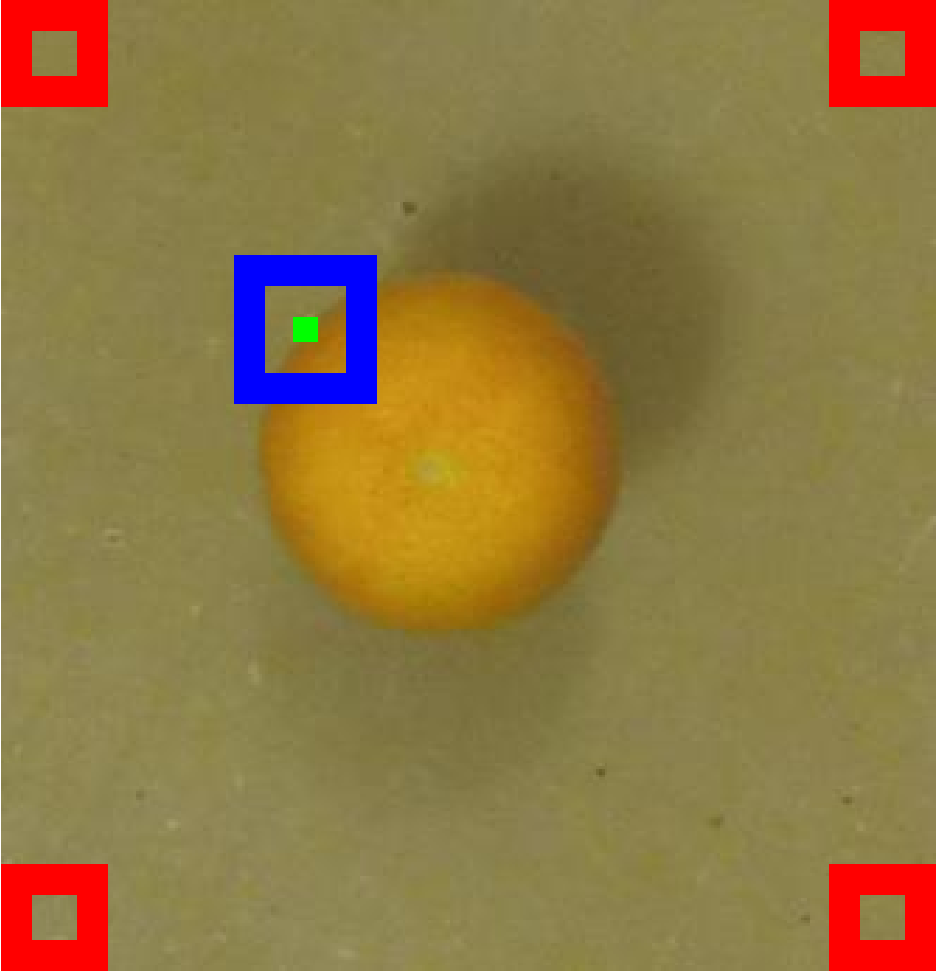
\includegraphics[width=\textwidth]{distdes_annotation_good_visualattn_seeds}
      \caption{}
      \label{fig:good_seg_visualattn_seeds}
  \end{subfigure}
  \begin{subfigure}[]{0.2\textwidth}
      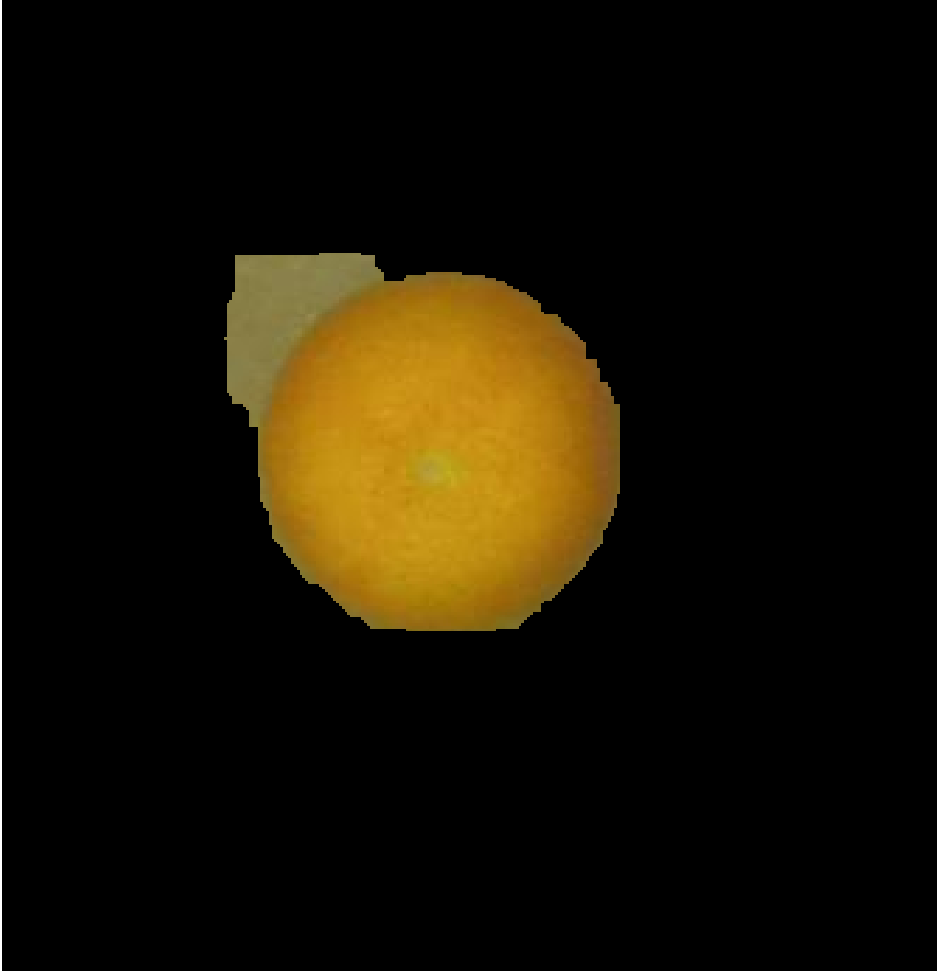
\includegraphics[width=\textwidth]{distdes_annotation_good_visualattn_segment}
      \caption{}
      \label{fig:good_seg_visualattn_seg}
  \end{subfigure}
  \begin{subfigure}[]{0.2\textwidth}
      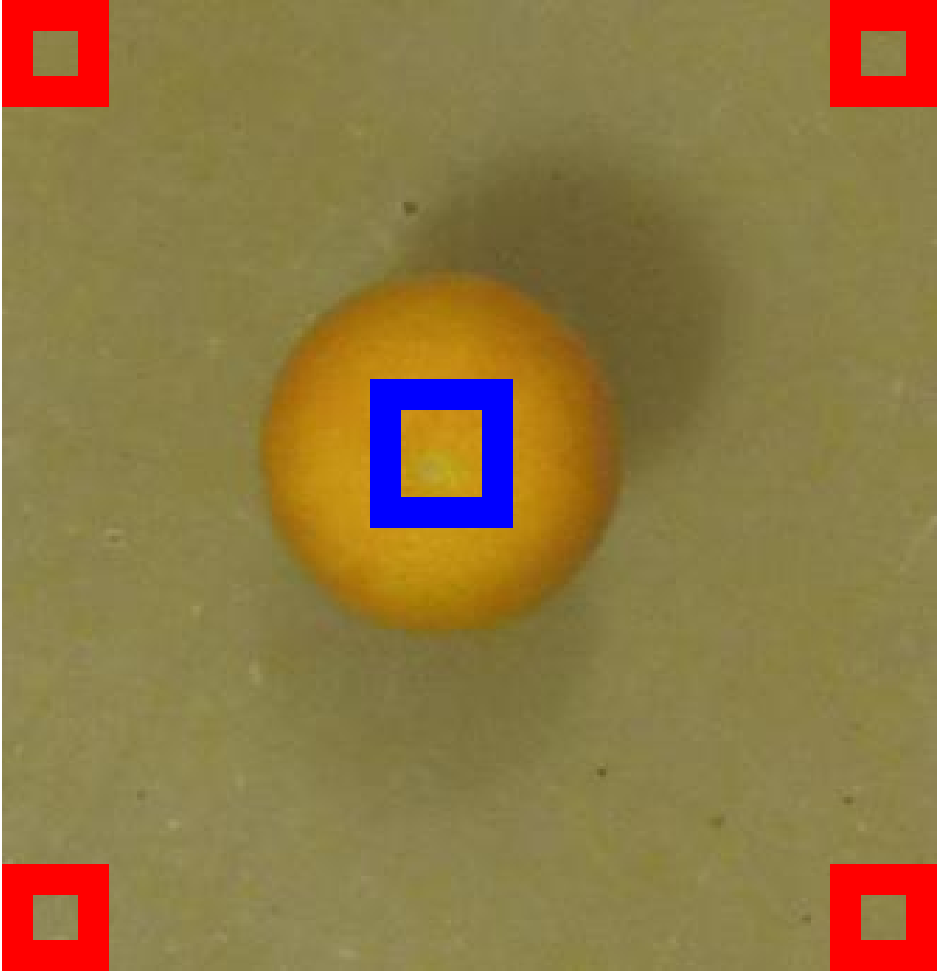
\includegraphics[width=\textwidth]{distdes_annotation_good_recursive_seeds}
      \caption{}
      \label{fig:good_seg_recursive_seeds}
  \end{subfigure}
  \begin{subfigure}[]{0.2\textwidth}
      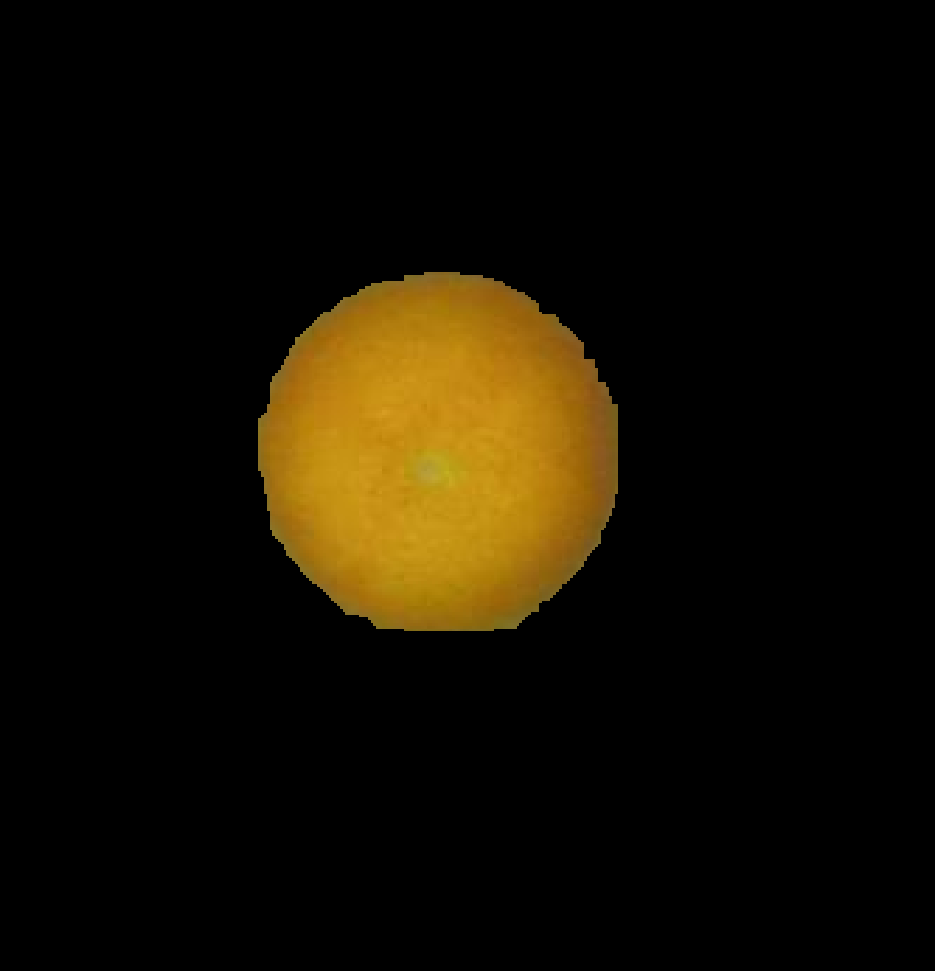
\includegraphics[width=\textwidth]{distdes_annotation_good_recursive_segment}
      \caption{}
      \label{fig:good_seg_recursive_seg}
  \end{subfigure}
\caption[Illustration of annotation process flow]{An illustration of operation of visual attention and recursive graphcut as a part of the annotation process flow is shown here. (\subref{fig:good_seg_visualattn_seeds}) shows the visual attention fixation as a green dot. Since the visual attention fixation is on the edge of the object, the foreground hypothesis rectangle shown in blue contains background pixels. When the graphcut algorithm operates on (\subref{fig:good_seg_visualattn_seeds}) utilizing the pixels inside the blue rectangle as the foreground seeds and the pixels inside the red rectangles as the background seeds, the resulting segmented foreground region is displayed in (\subref{fig:good_seg_visualattn_seg}). Due to the presence of background pixels in the input foreground seeds, the segmentation result obtained in (\subref{fig:good_seg_visualattn_seg}) is inaccurate. When recursive graphcut algorithm is 
applied, the blue foreground hypothesis rectangle eventually moves towards the center of the object (as seen in (\subref{fig:good_seg_recursive_seeds})) and no longer contains background pixels. With the updated foreground hypothesis rectangle after recursive graphcut segmentation, the improved segmentation result can be seen in (\subref{fig:good_seg_recursive_seg}).}
\label{fig:annotation_good_seg}
\end{figure*}	
%
The change in the blue foreground hypothesis rectangle after recursive graphcut segmentation and the resulting improved foreground labeling can be seen in Figure~\ref{fig:good_seg_recursive_seeds} and Figure~\ref{fig:good_seg_recursive_seg} respectively.
When the foreground region labels from the graphcut algorithm stabilize, it is unlikely that the foreground region will change after subsequent iterations. This stabilization condition captured in \eqref{eqn:seg_threshold}, indicates that the foreground region label hypothesis generated by graphcut has converged. In case the convergence condition in \eqref{eqn:seg_threshold} is not met after $N=5$ iterations, further recursion is abandoned and the labeling results available after $N$ iterations are adopted by default.

Though this process appears to be fully automated, there are cases where this automated segmentation fails. A case of segmentation failure could be due to visual attention picking up \emph{interesting} artifacts in the image that are not necessarily part of the specimen. There are also cases where the texture of the specimen is not uniform, in which case visual attention could be biased towards a specific part of the object. This could result in graphcut segmentation only identifying the sub-region of the specimen that biased the visual attention fixation. An instance of only segmenting a sub-region of the specimen is often seen in cases of strawberries, which are characterized by the occurrence of a green stalk along with a reddish pulp. Visual attention and graphcut could end up mistakenly segmenting either the green stalk or the red pulp only. This case is illustrated in Figure~\ref{fig:annotation_bad_seg}. The visual attention fixation shown by a green dot in Figure~\ref{fig:bad_seg_visualattn_seeds} is 
biased towards the green stalk region of the strawberry specimen. An application of recursive graphcut on this example only ends up segmenting the green stalk region as seen in Figure~\ref{fig:bad_seg_recursive_seg}. This error in segmentation can be rectified through inclusion of appropriate foreground seeds that are representative of the complete specimen, i.e. both the green stalk and the red pulp sub-regions in case of strawberry. Therefore, to prevent inaccurate segmentation from degrading the learning set, a manual verification process is added as the last step of this annotation process. During this process, for all failed instances of automated segmentation, the foreground and background seed pixels are manually set. 
%
\begin{figure*}
  \centering
  \begin{subfigure}[]{0.2\textwidth}
      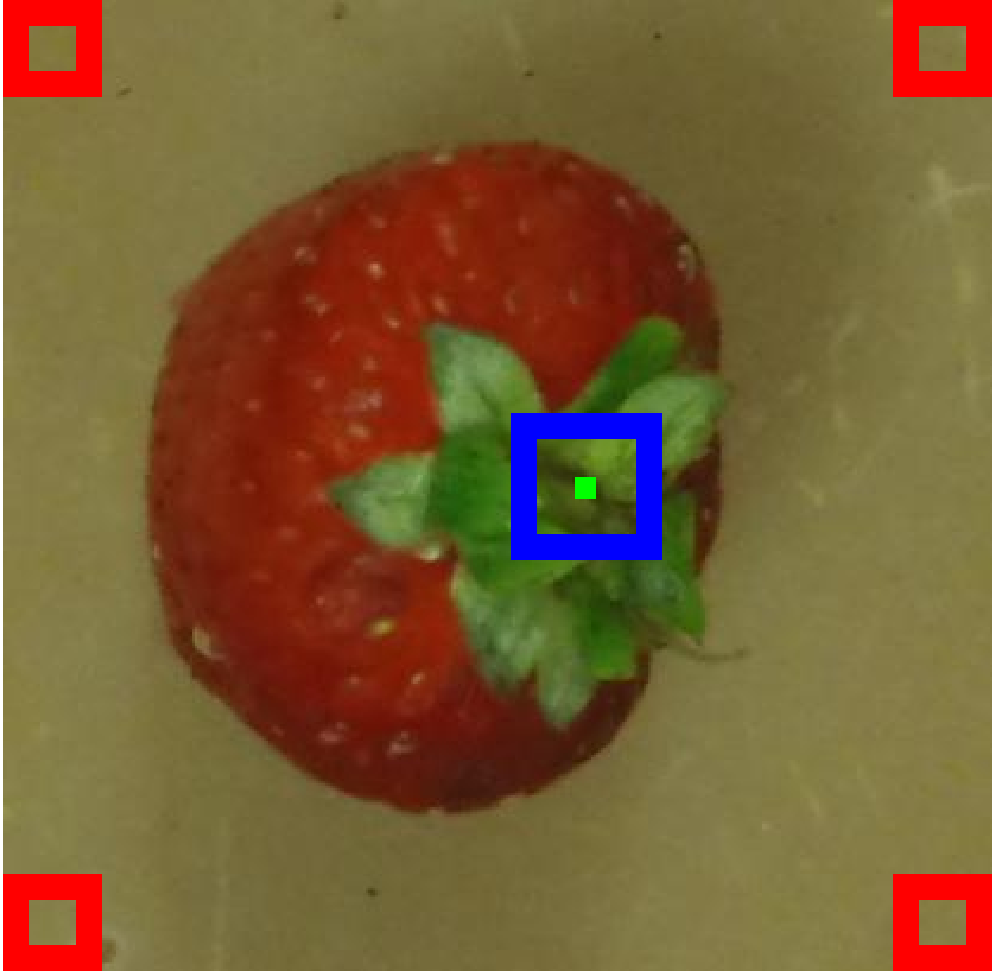
\includegraphics[width=\textwidth]{distdes_annotation_bad_visualattn_seeds}
      \caption{}
      \label{fig:bad_seg_visualattn_seeds}
  \end{subfigure}
  \begin{subfigure}[]{0.2\textwidth}
      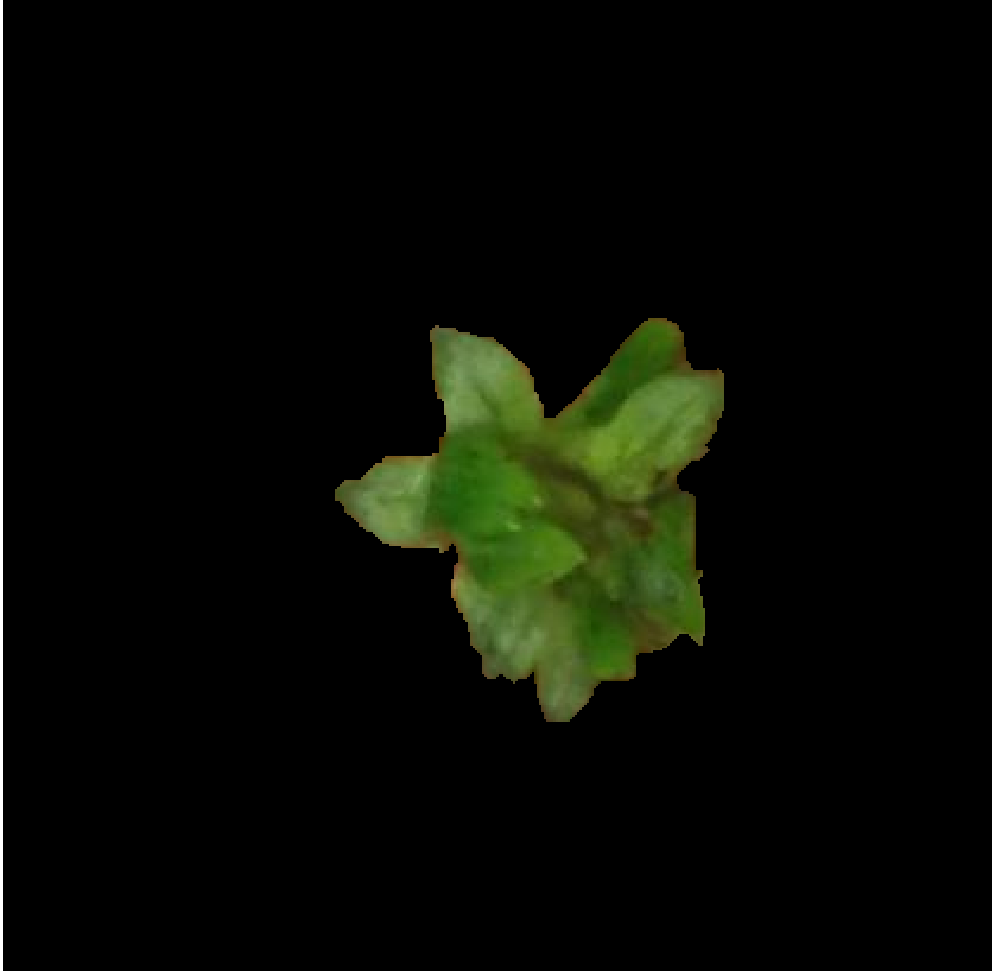
\includegraphics[width=\textwidth]{distdes_annotation_bad_recursive_segment}
      \caption{}
      \label{fig:bad_seg_recursive_seg}
  \end{subfigure}
\caption[Illustration of a case where automated annotation process fails]{An illustration of a case where automated annotation process fails, and human verification and correction is required. The visual attention fixation shown as a green dot in (\subref{fig:good_seg_visualattn_seeds}) is biased towards the green stalk region of the strawberry. Since this strawberry specimen exhibits binary texture--green stalk and red pulp, the combined visual attention and graphcut automated annotation approach ends up segmenting only the stalk sub-region of this strawberry specimen (see (\subref{fig:bad_seg_recursive_seg})). Such cases of failure calls for human verification and correction of foreground seeds to enable graphcut algorithm to segment the whole strawberry specimen.} 
\label{fig:annotation_bad_seg}
\end{figure*}	
%

This final manual verification and correction process requires human effort. However, during experiments it was noted that a very small percentage of cases needed corrective action. In summary, this semi-automated annotation process is relatively less cumbersome than a fully manual annotation effort. An illustration of the output of this annotation process for a single specimen of orange is shown in Figure~\ref{fig:orange_segment_height_montage}. Figure~\ref{fig:orange_segment_height_montage} represents a montage of 13 images of an orange specimen with the top-left component showing the segmented foreground from the image captured 32 inches away from the orange specimen. Likewise, the bottom-most row shows the image that was captured 8 inches away from the specimen. The montage in Figure~\ref{fig:orange_segment_height_montage} is arranged such that the 13 images, from left to right, are in the decreasing order of the heights from which the images were capture. This sequence of images in the montage wraps 
around after 
every 4 images resulting in four rows to represent 13 images.
%
\begin{figure*}
  \centering
  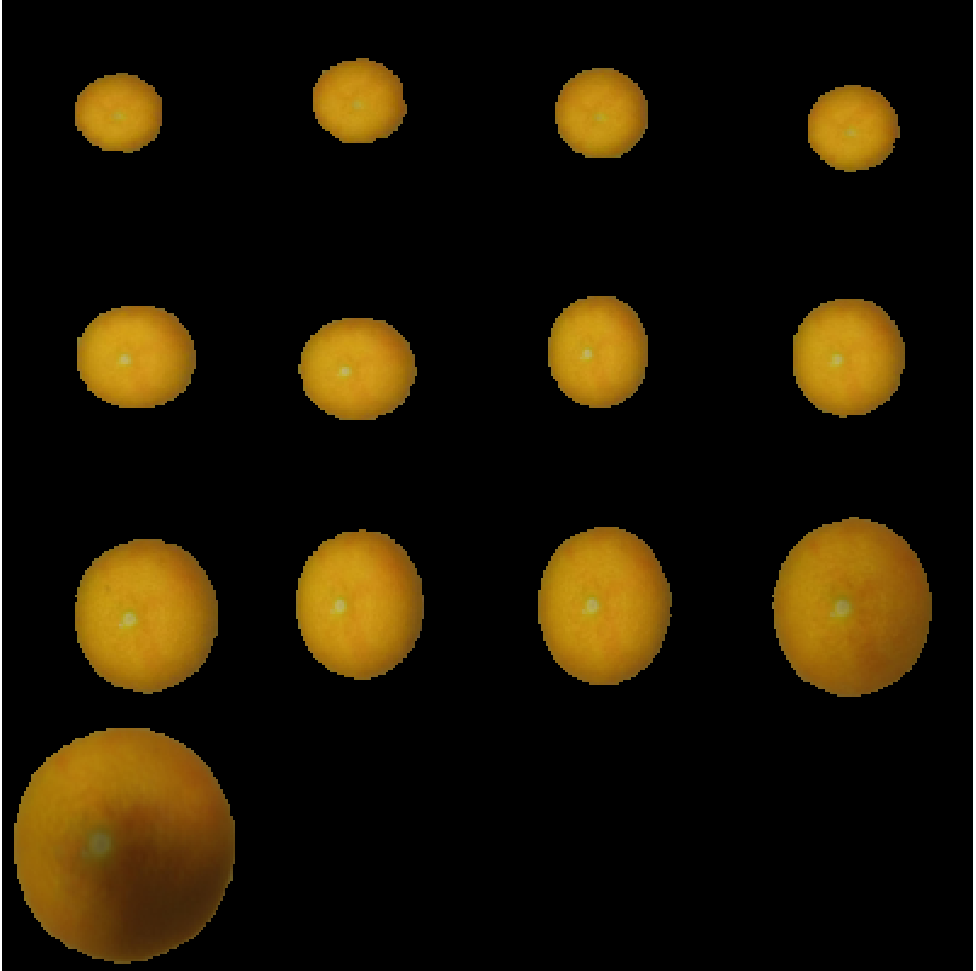
\includegraphics[width=\textwidth]{orange_height_segment_montage}
  \caption[Annotation output for a single specimen]{The output of the annotation process showing a montage of the segmented foreground from a set of 13 images that belong to a single orange specimen. The left-top montage component is the image of the orange specimen captured 32 inches from the ground. The montage components arranged from left to right (with wrap-around after every 4 images) to progressively show images that were captured closer to the orange specimen. The closest image that was captured is 8 inches away from the specimen and is shown in the bottom-most row.} 
  \label{fig:orange_segment_height_montage}
\end{figure*}	
%


\subsection{Learning}

\begin{enumerate}
	\item Learning phase of a machine learning method involves parsing labeled data to identify features that can reliably indicate the identity of an object.
	
	\item In this method, we extract features from multiple images of a target acquired from different heights.
	
	\item Manual intervention is minimized by using visual attention to aid the detection of interesting regions in the image that could be targets.
	
	\item Graphcut is then segments the detected interesting regions using the the visual attention fixations as foreground seeds.
	
	\item In case of failure of this automated detection and segmentation approach seeds are selected manually for the graphcut algorithm to operate on.
	
	\item A histogram based distance metric is used to compare the images with segmented object and the unsegmented image corresponding to each of the 13 samples available for each target object.
	
	\item The information available from the histogram distance metric for data collected from different heights is used to construct a single feature descriptor for each instance of the target.
	
	\item The feature descriptor from all target instances are then combined to produce a feature distribution for the target.
\end{enumerate}


The learning phase of a machine learning based object recognition method involves identifying patterns in the data that represent the presence of an object. The information fed to a machine learning algorithm is a pre-specified labeling of the data into foreground and background. The responsibility of the learning method here is to identify patterns in designated foreground regions, using information from labeled background to reject false positives. The patterns identified by the learning algorithm are then channeled into the construction of a classifier that is capable of identifying foreground pixels from an image.

In the machine learning technique proposed in this chapter, instead of using individual images with annotations of foreground and background, a collection of 13 images each featuring the same specimen from a known height is utilized. The goal is to encode the variation in appearance of a specimen from different heights to build a robust object recognition classifier. Height offers an additional dimension in the feature space for the learning algorithm to capitalize on.

This object recognition algorithm is designed to operate on images without prior segmentation. That is, the features used in this algorithm should be sufficiently generic to capture the appearance of an object directly from an image without foreground segmentation. To achieve this, we use the histogram signatures (described in Section~\ref{sec:hist_signature}) to extract information from an image in \gls{hsi} colorspace. The histogram information from multiple specimens of the same object class is then combined to generate a feature distribution. The details of this process are described below.

\subsubsection{Feature Distribution}
\label{sec:distdes_feature_distr}

The first step in computing feature distribution is the computation of the hue, saturation and intensity histogram signatures on the labeled foreground pixels in the learning dataset. The parameters chosen for the histogram signature computation are the number of equally spaced histogram bins, $|\mathcal{B}|=256$, and the upper bound on the number of pixels affected by noise, $e=5\%$. Using these parameters the histogram signatures for all three components of the \gls{hsi} colorspace are calculated for all 13 height-tagged images of a specimen. Note that this histogram signature computation only utilizes the labeled foreground pixels in the image. Let the histogram signature of the labeled foreground for specimen $k$, with height tag $h$, belonging to class $c$, on the color component $f\in\{H \text{ hue}, S \text{ saturation}, I \text{ intensity}\}$ be represented as $\mathcal{H}^{c_{hk}}_f$. Since there are 3 color components, we generate 3 histogram signatures per height-tagged specimen image. If we 
consider all the 13 height-tagged images available for a specimen, the total histogram signatures now available is 39 ($13 \times 3$).

In the next stage of the learning process, the histogram signatures $\mathcal{H}^{c_{hk}}_f$ from all specimens belonging to a single object class are combined to generate a generalized histogram signature for the object class.
In order to achieve this, the mean of all histogram signatures corresponding to a specific height-tag from all specimens of a class are combined. In other words, the mean $\bar{\mathcal{H}}^{c_{h}}_f$ of all histogram signatures with  height-tag $h$ are computed by taking the mean of individual components of the $256$-dimensional vectors of sequence-of-histogram signatures $\mathcal{H}^{c_{h1}}_f, \mathcal{H}^{c_{h2}}_f, \mathcal{H}^{c_{h3}}_f, \ldots, \mathcal{H}^{c_{hm}}_f$, where $m$ is the number of specimens of class $c$ available in the learning dataset. Technically, the computation of the $j$-th component of the $256$-dimensional mean histogram $\bar{\mathcal{H}}^{c_{h}}_f$ is found as
\begin{align}
 \left[\bar{\mathcal{H}}^{c_{h}}_f\right]_j=\frac{1}{m}\sum_{k=1}^{m} \left[ \mathcal{H}^{c_{hk}}_f \right]_j.
\end{align}
Since there are 13 different height-tags along with 3 different color components, each object class $c$ is represented by a sequence of $39\, (13 \times 3)$ histogram signatures, which will be collectively referred to as $\bar{\mathcal{H}}^{c}$.

The sequence of $39$ histogram signatures $\bar{\mathcal{H}}^{c}$ captures the generalized appearance of the objects of class $c$. Its important to note that the data used to compute this generalized histogram signature are composed of foreground pixels of object specimens only, without any background information. If we are to use such a generalized histogram signature generated only from foreground information for classifying objects, it is necessary to pre-process an image to detect and segment objects present in the images before this generalized histogram signature $\bar{\mathcal{H}}^{c}$ can be used for classification purposes. However, one of the goals of this work is to avoid segmentation while attempting classification of objects from images. To realize this goal, we revisit the learning dataset, and use the background information to build a representation that captures how inclusion of background pixels to different individual histogram signatures affects the generalized histogram signature $\bar{
\mathcal{H}}^{c}$ of class $c$. 

In order to use background information for building such a classifier, we first generate another set of histogram signatures.
For specimen $k$ of class $c$ from the learning dataset, we compute a sequence of $39$ histogram signatures similar to the computation involved in $\mathcal{H}^{c_{hk}}_f$, but now utilizing all pixels in the image instead of just the foreground pixels. This set of 39 histograms $\ddot{\mathcal{H}}^{c_{k}}$ for specimen $k$ of class $c$ is given by
\begin{align}	\label{eqn:hist_signature}
 \ddot{\mathcal{H}}^{c_{k}} = \ddot{\mathcal{H}}^{c_{hk}}_f \Big|_{h\times f}\enspace ,
\end{align}
%
where $h\in\{8,10,12, \ldots,32\}$ and $f\in\{H,S,I\}$.

Once we have the sequence of histogram signatures $\ddot{\mathcal{H}}^{c_{k}}$ of specimen $k$ belonging to class $c$, along with the generalized histogram signature $\bar{\mathcal{H}}^{c}$ of class $c$, a numeric distance measure $D$ between the histogram signatures can be computed. If we have a series of such distance measures evaluated for a collection of specimens of class $c$, a distribution of these distance measures can be generated. This distribution 
of distance measures encodes the variability in generalized histogram signature $\bar{\mathcal{H}}^{c}$ induced by the presence of background pixels along with foreground pixels. In effect, this offers a way to check images for the presence of an object of class $c$ without any prior segmentation of foreground pixels. The distance measure is the standard \emph{$L_2$-norm} between two vectors.
%
\begin{align}	\label{eqn:hist_signature_dist}
 d_{chfk} = D(\bar{\mathcal{H}}^{c_{h}}_f, \ddot{\mathcal{H}}^{c_{hk}}_f) 
 = \sqrt{\sum_{j=1}^{|B|}\Bigg(\left[\bar{\mathcal{H}}^{c_{h}}_f\right]_j
 -\left[\ddot{\mathcal{H}}^{c_{hk}}_f\right]_j\Bigg)^2}
\end{align}

Since there are 39 histograms in total, we get a sequence of 39 $d_{chfk}$ values for the $k$-th specimen of class $c$, and this sequence is represented as
%
\begin{align}	\label{eqn:dist_sequence}
 D_{ck}=d_{chfk}\Big|_{h\times f}\enspace ,
\end{align}
%
where $h=\{8,10,12, \ldots,32\}$ and $f=\{H,S,I\}$.

A sequence of distance measures $D_{ck}$ for each specimen $k$ among the $m$ specimens of class $c$ provides a representation of a feature vector of size 39 that describes the appearance of an image that contains a specimen of class $c$. If we consider the feature vectors of all the $m$ available specimens $D_{c1},D_{c2},\ldots,D_{cm}$, a feature distribution sequence $F_c$ that represents the appearance of images containing objects of class $c$ can be formulated. Lets assume that the $m$ values $d_{chf1}, d_{chf2},\ldots,d_{chfm}$ are drawn from a normal distribution 
%
\begin{align}
 F_{chf}\sim &\mathcal{N}(\mu_{chf},\sigma^2_{chf})\label{eqn:normal_distr}\\
 \mu_{chf}= &\frac{\sum_{k=1}^m d_{chfk}}{m}\label{eqn:normal_mean}\\
 \sigma^2_{chf}= &\frac{\sum_{k=1}^m (d_{chfk}-\mu_{chf})^2}{m-1}\label{eqn:normal_stddev}\enspace .
\end{align}
%
Then the feature distribution sequence
\begin{align}	\label{eqn:feat_distribution}
 F_c=F_{chf}\Big|_{h \times f}
\end{align}
can be represented as a sequence of 39 distributions,
where $h\in\{1,2,\ldots,13\}$ and $f\in\{H,S,I\}$. 

For the two classes of objects, strawberries and oranges with 11 specimens each, the respective feature distributions $F_s$ and $F_o$ can thus be computed. The feature distributions $F_s$ and $F_o$ are shown in Figure~\ref{fig:feat_distr}. The 39 distributions (see \eqref{eqn:feat_distribution}) in the distribution sequence are shown along the $x$-axis. Each distribution here is represented by a dot and a bar adjoining it. The dot corresponds to the mean and the bar corresponds to the 95\% confidence interval, or the $2\sigma$ standard deviation interval of the distribution shown in \eqref{eqn:normal_distr}.
%
\begin{figure*}
  \centering
  \begin{subfigure}[]{0.8\textwidth}
      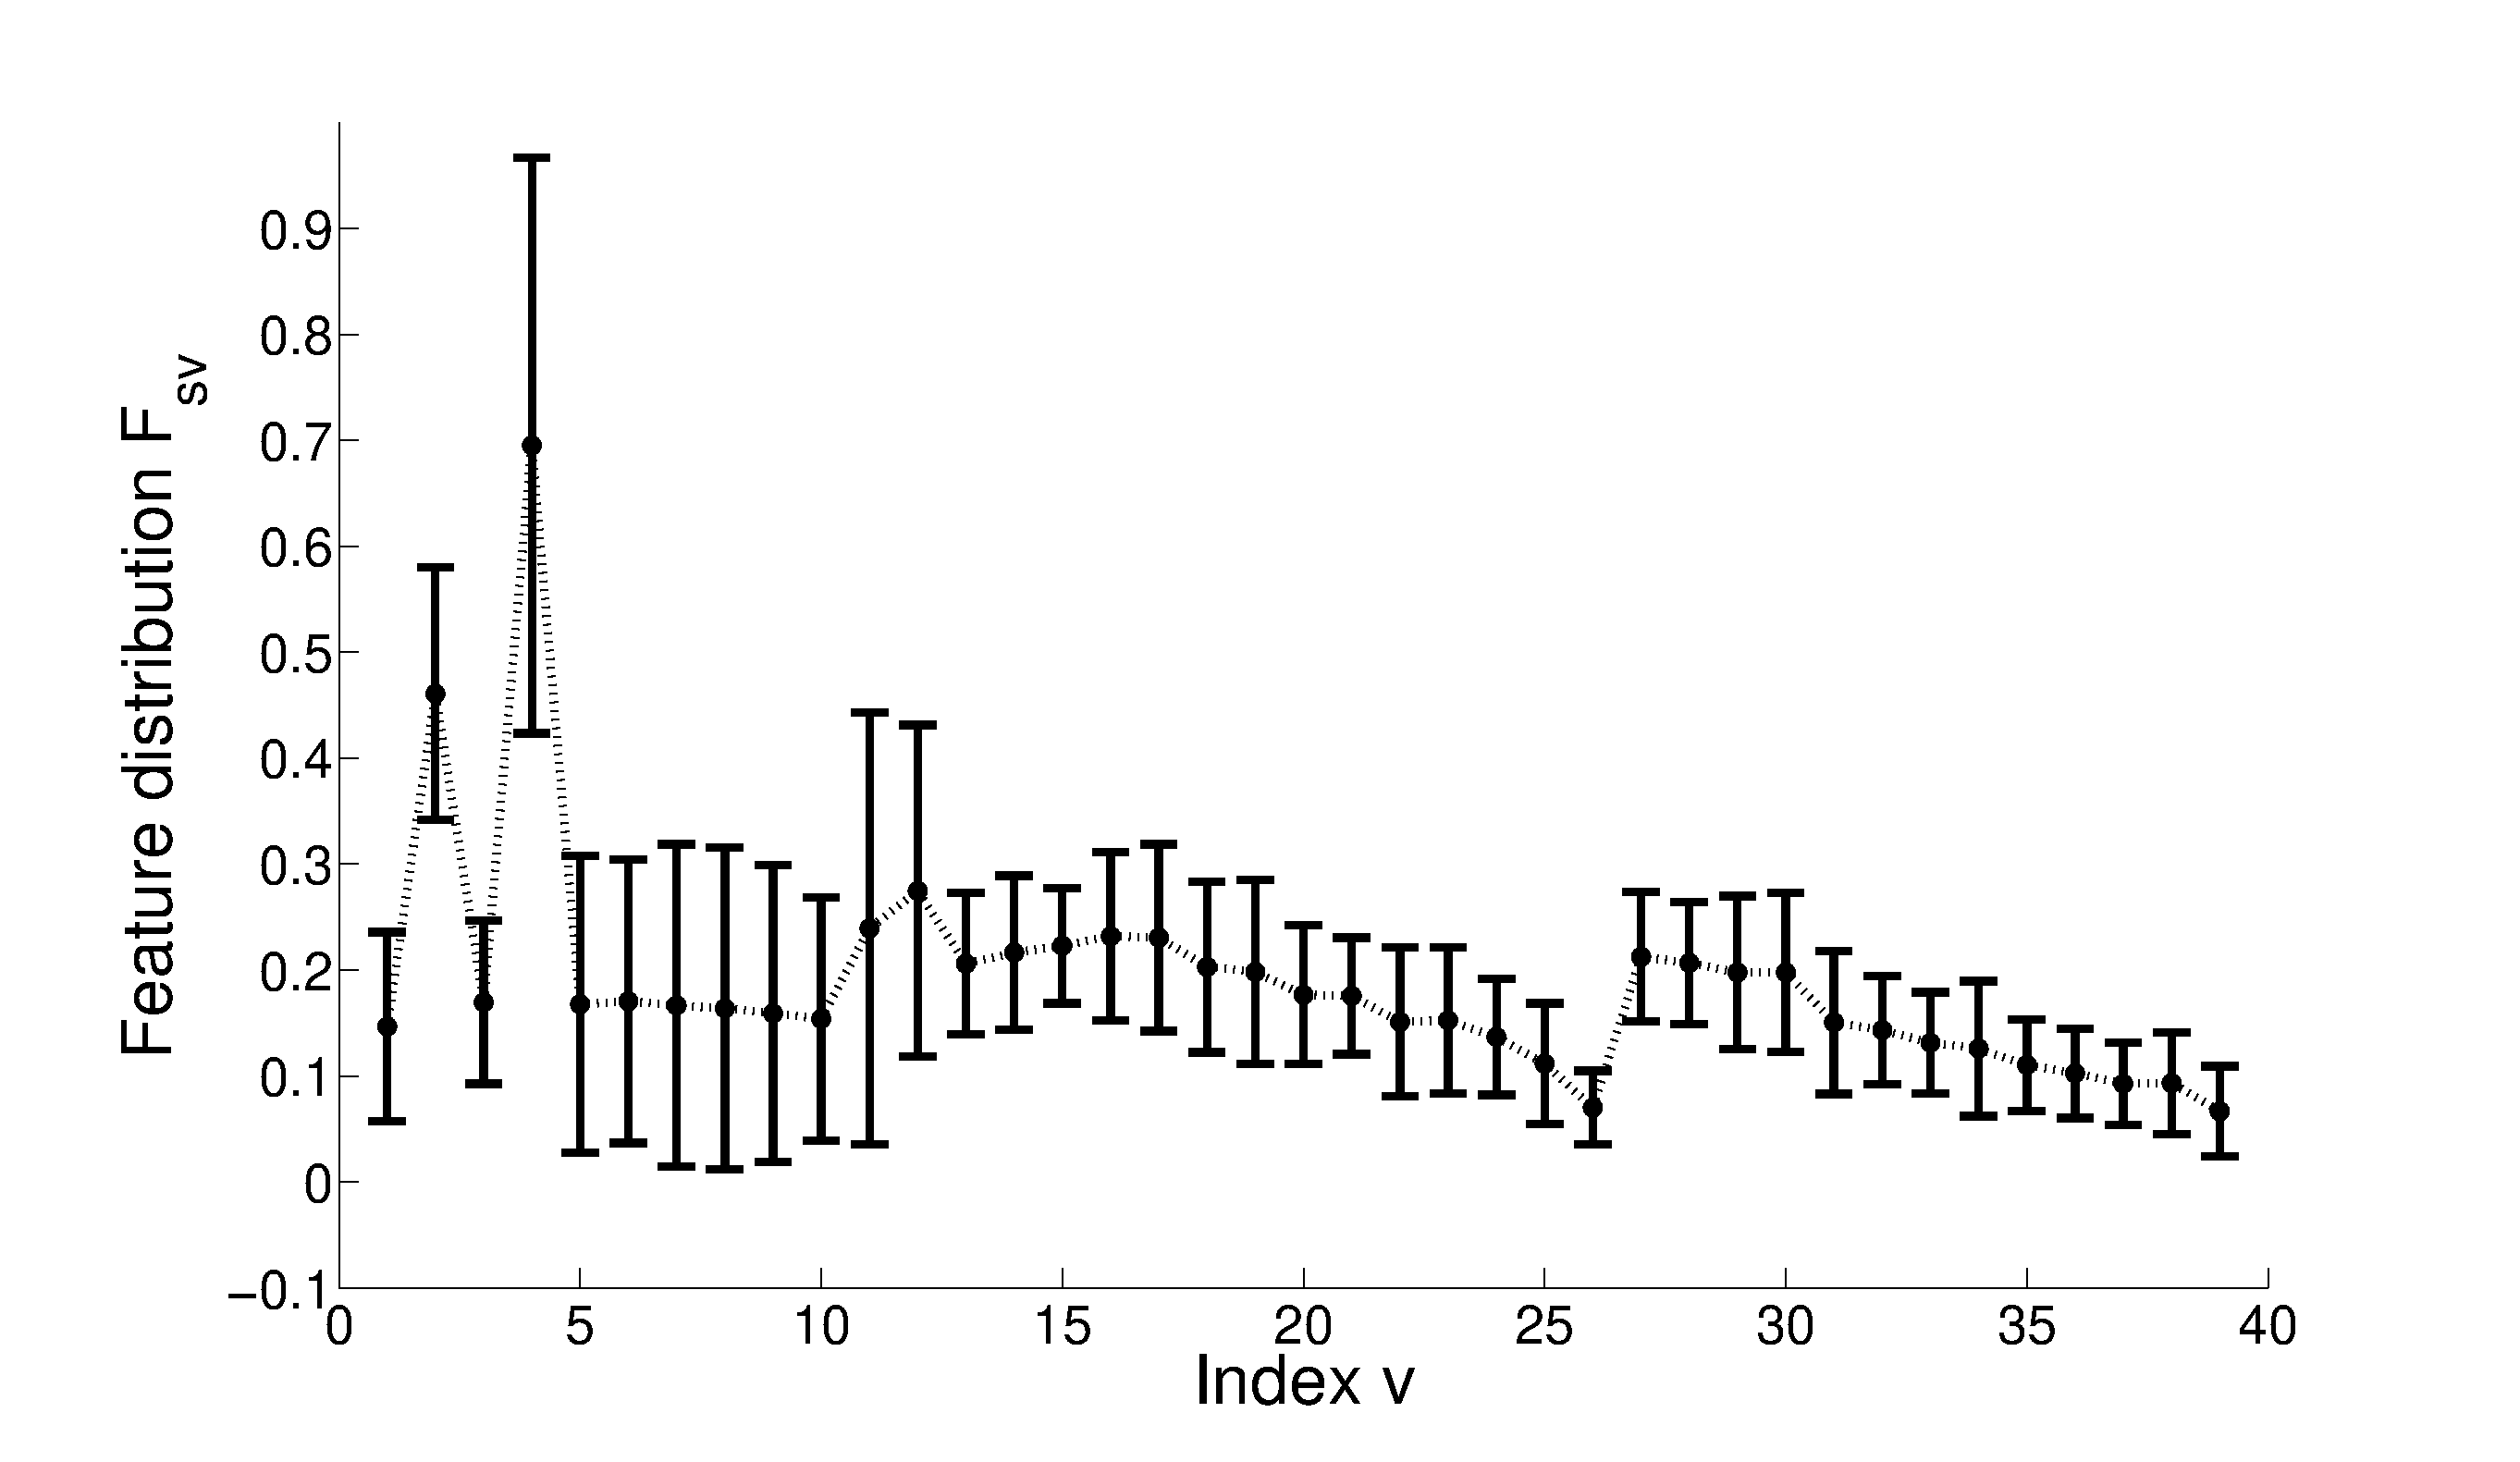
\includegraphics[width=\textwidth]{strawberry_learning_feature_distribution}
      \caption{}
      \label{fig:feat_distr_strawberry}
  \end{subfigure}
  \begin{subfigure}[]{0.8\textwidth}
      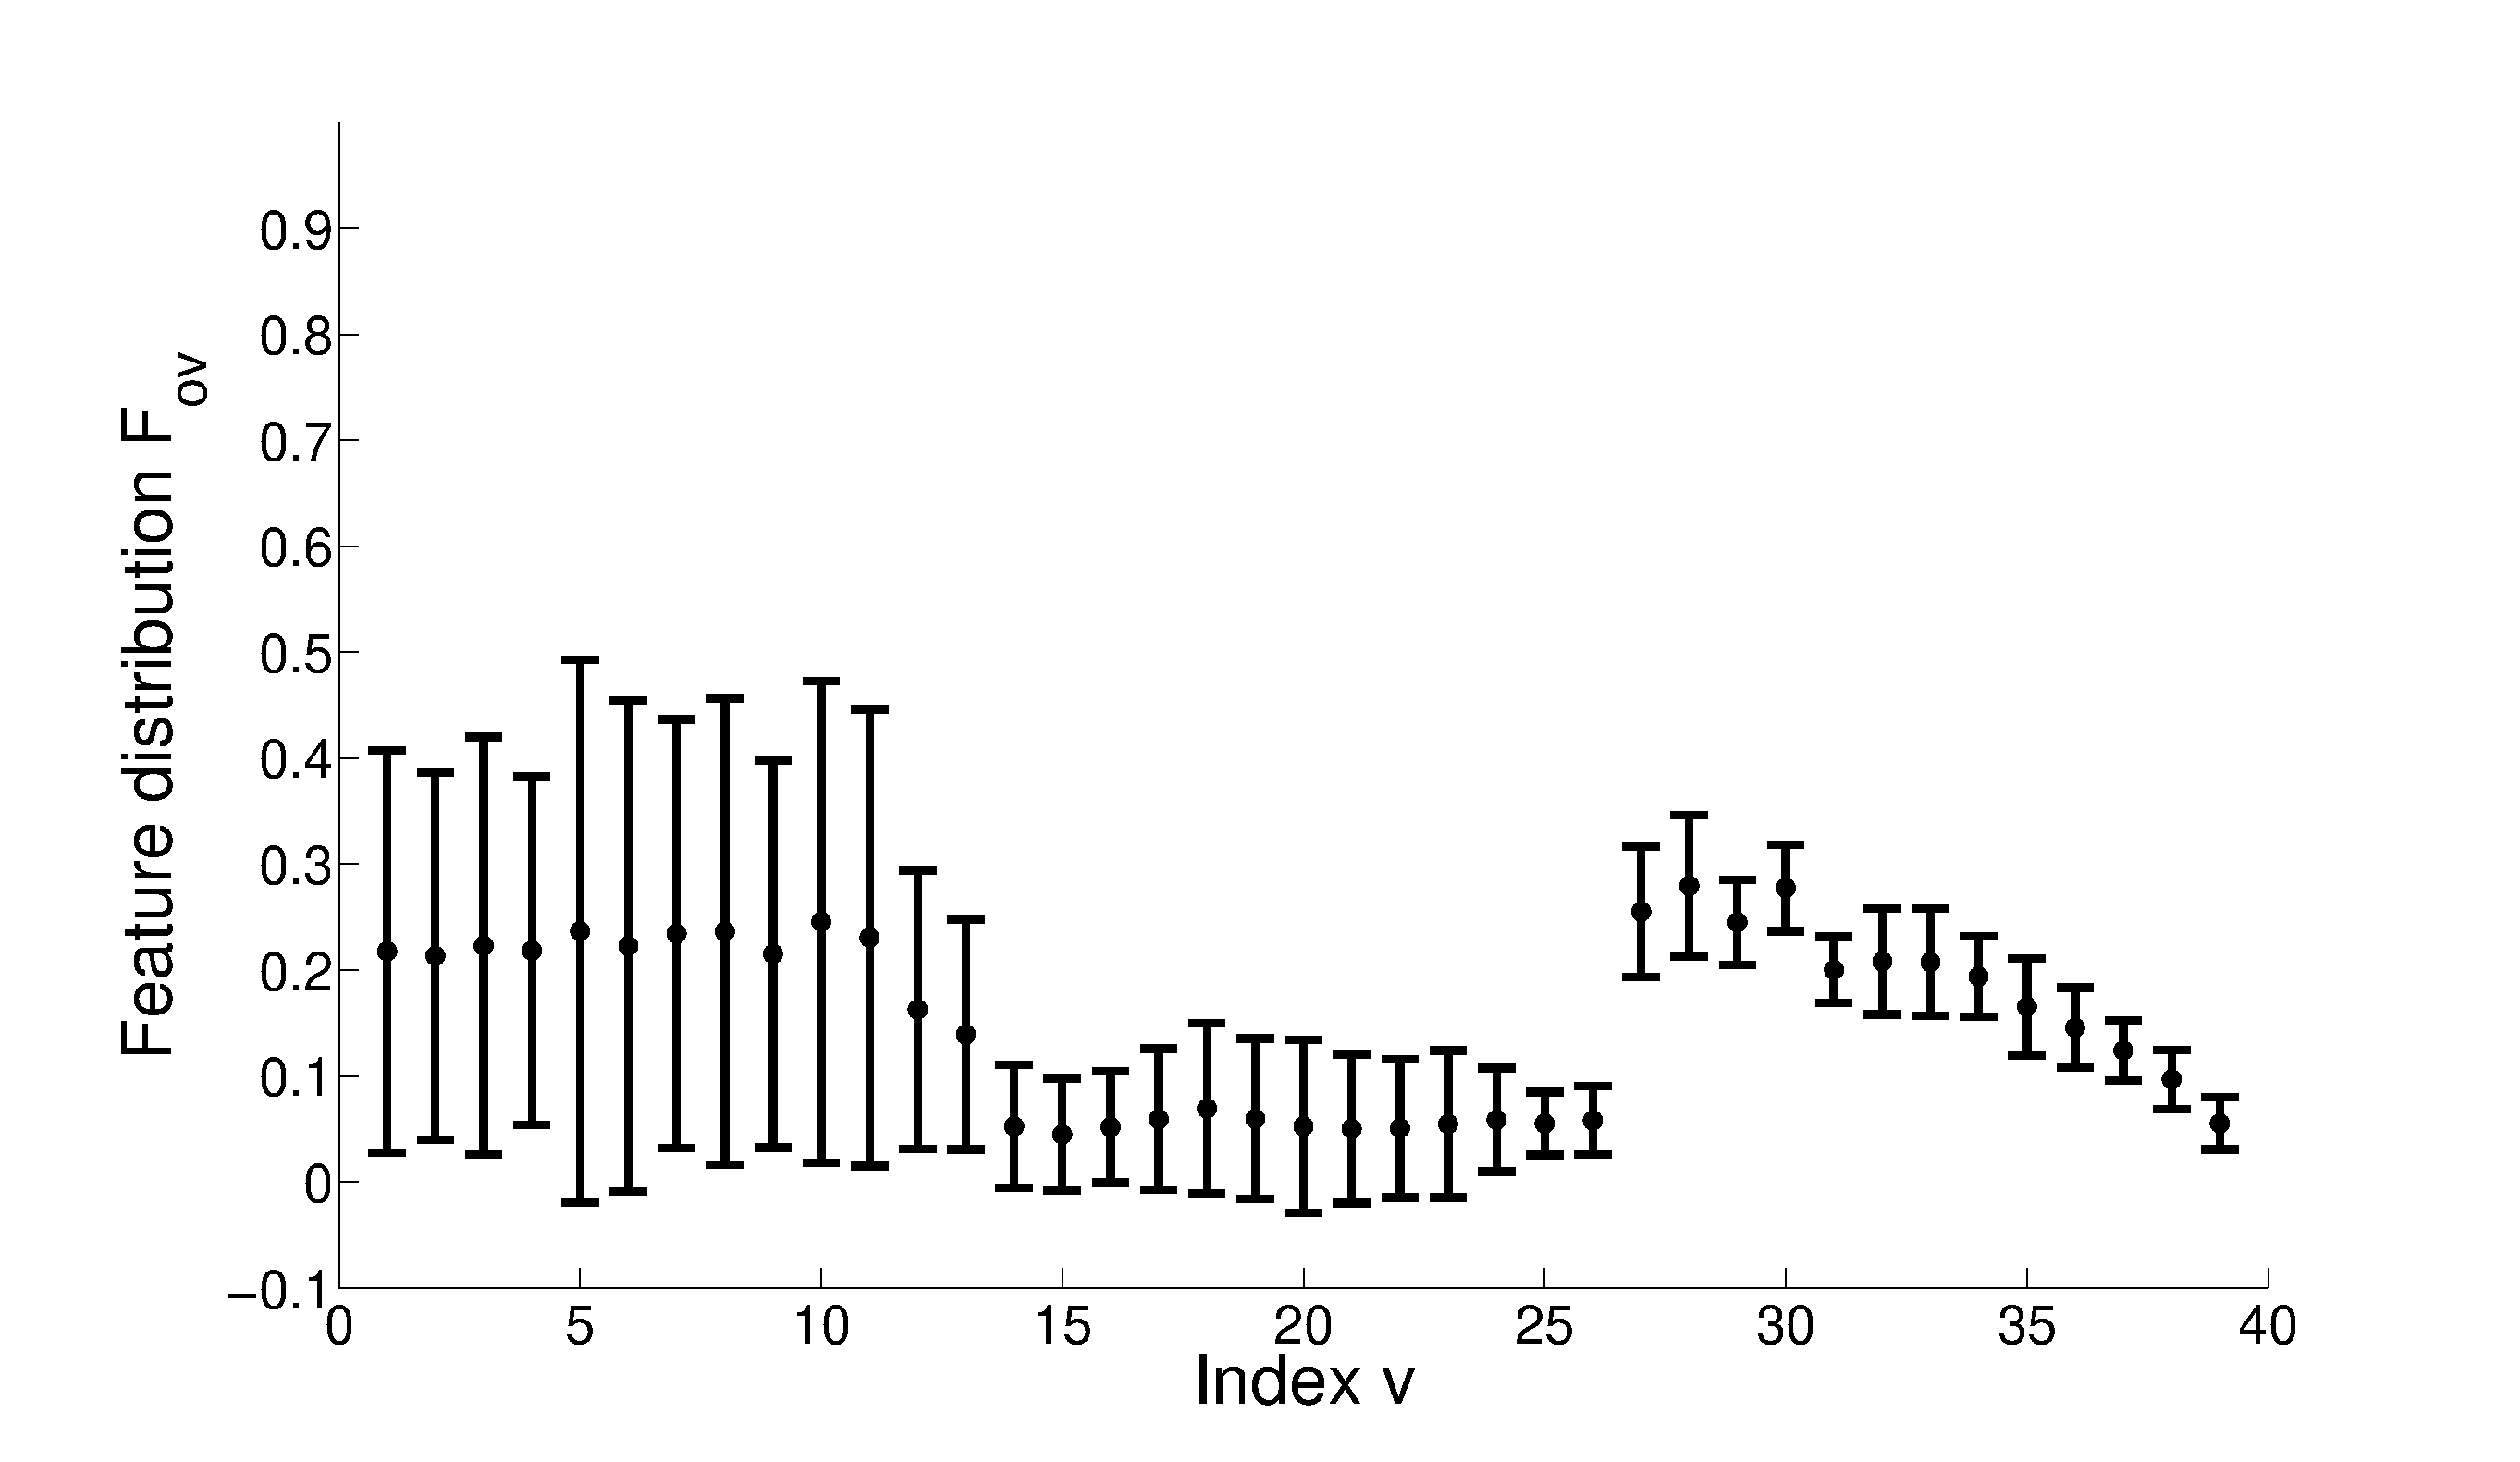
\includegraphics[width=\textwidth]{orange_learning_feature_distribution}
      \caption{}
      \label{fig:feat_distr_orange}
  \end{subfigure}
\caption[Feature distribution]{Strawberry feature distribution sequence $F_s$ (\subref{fig:feat_distr_strawberry}) and orange feature distribution sequence $F_o$ (\subref{fig:feat_distr_orange}) generated from 11 strawberry specimens and 11 orange specimens. All 39 distributions indexed by $v$ are shown along the $x$-axis. The  mean of each distribution is shown as a dot along with the 95\% confidence interval shown as a bar.}
\label{fig:feat_distr}
\end{figure*}	
%

This feature distribution $F_c$, which comprises a sequence of 39 distributions, offers a way to test for the presence of an object of class $c$ in an image without prior segmentation. In essence, the testing for the presence of an object can be broken down into 39 individual hypothesis tests. Each hypothesis test checks whether a certain colorspace-specific height-tagged image containing an object satisfies a specific distribution, among the 39 distributions in $F_c$. Not all of the 39 hypothesis tests might be equally informative-- some of them could be more relevant than others. To this end, a weighting factor $w_{v}$ can be attached to the $v$-th element in feature distribution sequence $F_c$.  The details involved in the computation of these weight factors is described below.

\subsubsection{Feature Weights}
\label{sec:distdes_feat_wts}

The feature weights offer a way to weight each distribution in the feature distribution sequence $F_c$. In case of a binary classification problem between objects of class $p$ and $q$, we choose the feature weights such that the distributions in the sequence with lower intra-class variance are weighted higher compared to other distributions. Additionally, the magnitude of the overlap between identical indexed distributions in $F_p$ and $F_q$ also influences the weights. In the rest of this section the formulation of these feature weights is discussed.

For object class $p$ and object class $q$, the corresponding feature distribution sequences $F_p$ and $F_q$ are in both cases sequences of 39 normal distributions. Let the $v$-th component of sequence $F_p$ be denoted $F_{pv}\sim\mathcal{N}(\mu_{pv},\sigma^2_{pv})$.
The the 95\% confidence interval of $F_{pv}$ is given by
%
\begin{align}	\label{eqn:conf_interval}
C^{0.95}_{F_{pv}}=[\mu_{pv}-2 \times \sigma_{pv},\, \mu_{pv}+2 \times \sigma_{pv}]\enspace .
\end{align}
%
The weight $w_{pv}$ of the $v$ component of $F_p$ is given by
\begin{align}
 w'_{pv}= & \frac{1}{(1+ |C_{F_{pv}} \cap C_{F_{qv}}| )\times \sigma_{pv}} \label{eq:feat_wt}\\
 w_{pv}= & \frac{w'_{pv}}{\sum_{j} w'_{pj}} \label{eqn:feat_wt_norm}
\end{align}
where $|C_{F_{pv}} \cap C_{F_{qv}}|$ corresponds to the length of the interval obtained after the intersection of intervals $C_{F_{pv}}$ and $C_{F_{qv}}$. The first term in the denominator of \eqref{eq:feat_wt}, $1+ |C_{F_{pv}} \cap C_{F_{qv}}|$, penalizes distributions whose confidence intervals share common positions with an identical indexed distribution in the other class. In other words, this term penalizes distribution $F_{pv}$ whose confidence interval overlaps with intervals of an identical indexed distribution $F_{qv}$. The second term in the denominator of \eqref{eq:feat_wt}, $\sigma_{pv}$, penalizes distributions with high intra-class variance. Ultimately, the weights are normalized as shown in \eqref{eqn:feat_wt_norm}. The 39 feature weights thus computed for a class will collectively be referred to as $W_c$. For the binary classification problem, between strawberry and orange specimens, the weight factors computed using \eqref{eqn:feat_wt_norm} are shown in the bar plot in Figure~\ref{fig:feat_weights}. The black bars show the strawberry 
class 
weights and the red 
bars show the corresponding orange class weights.
%
\begin{figure}
  \centering
  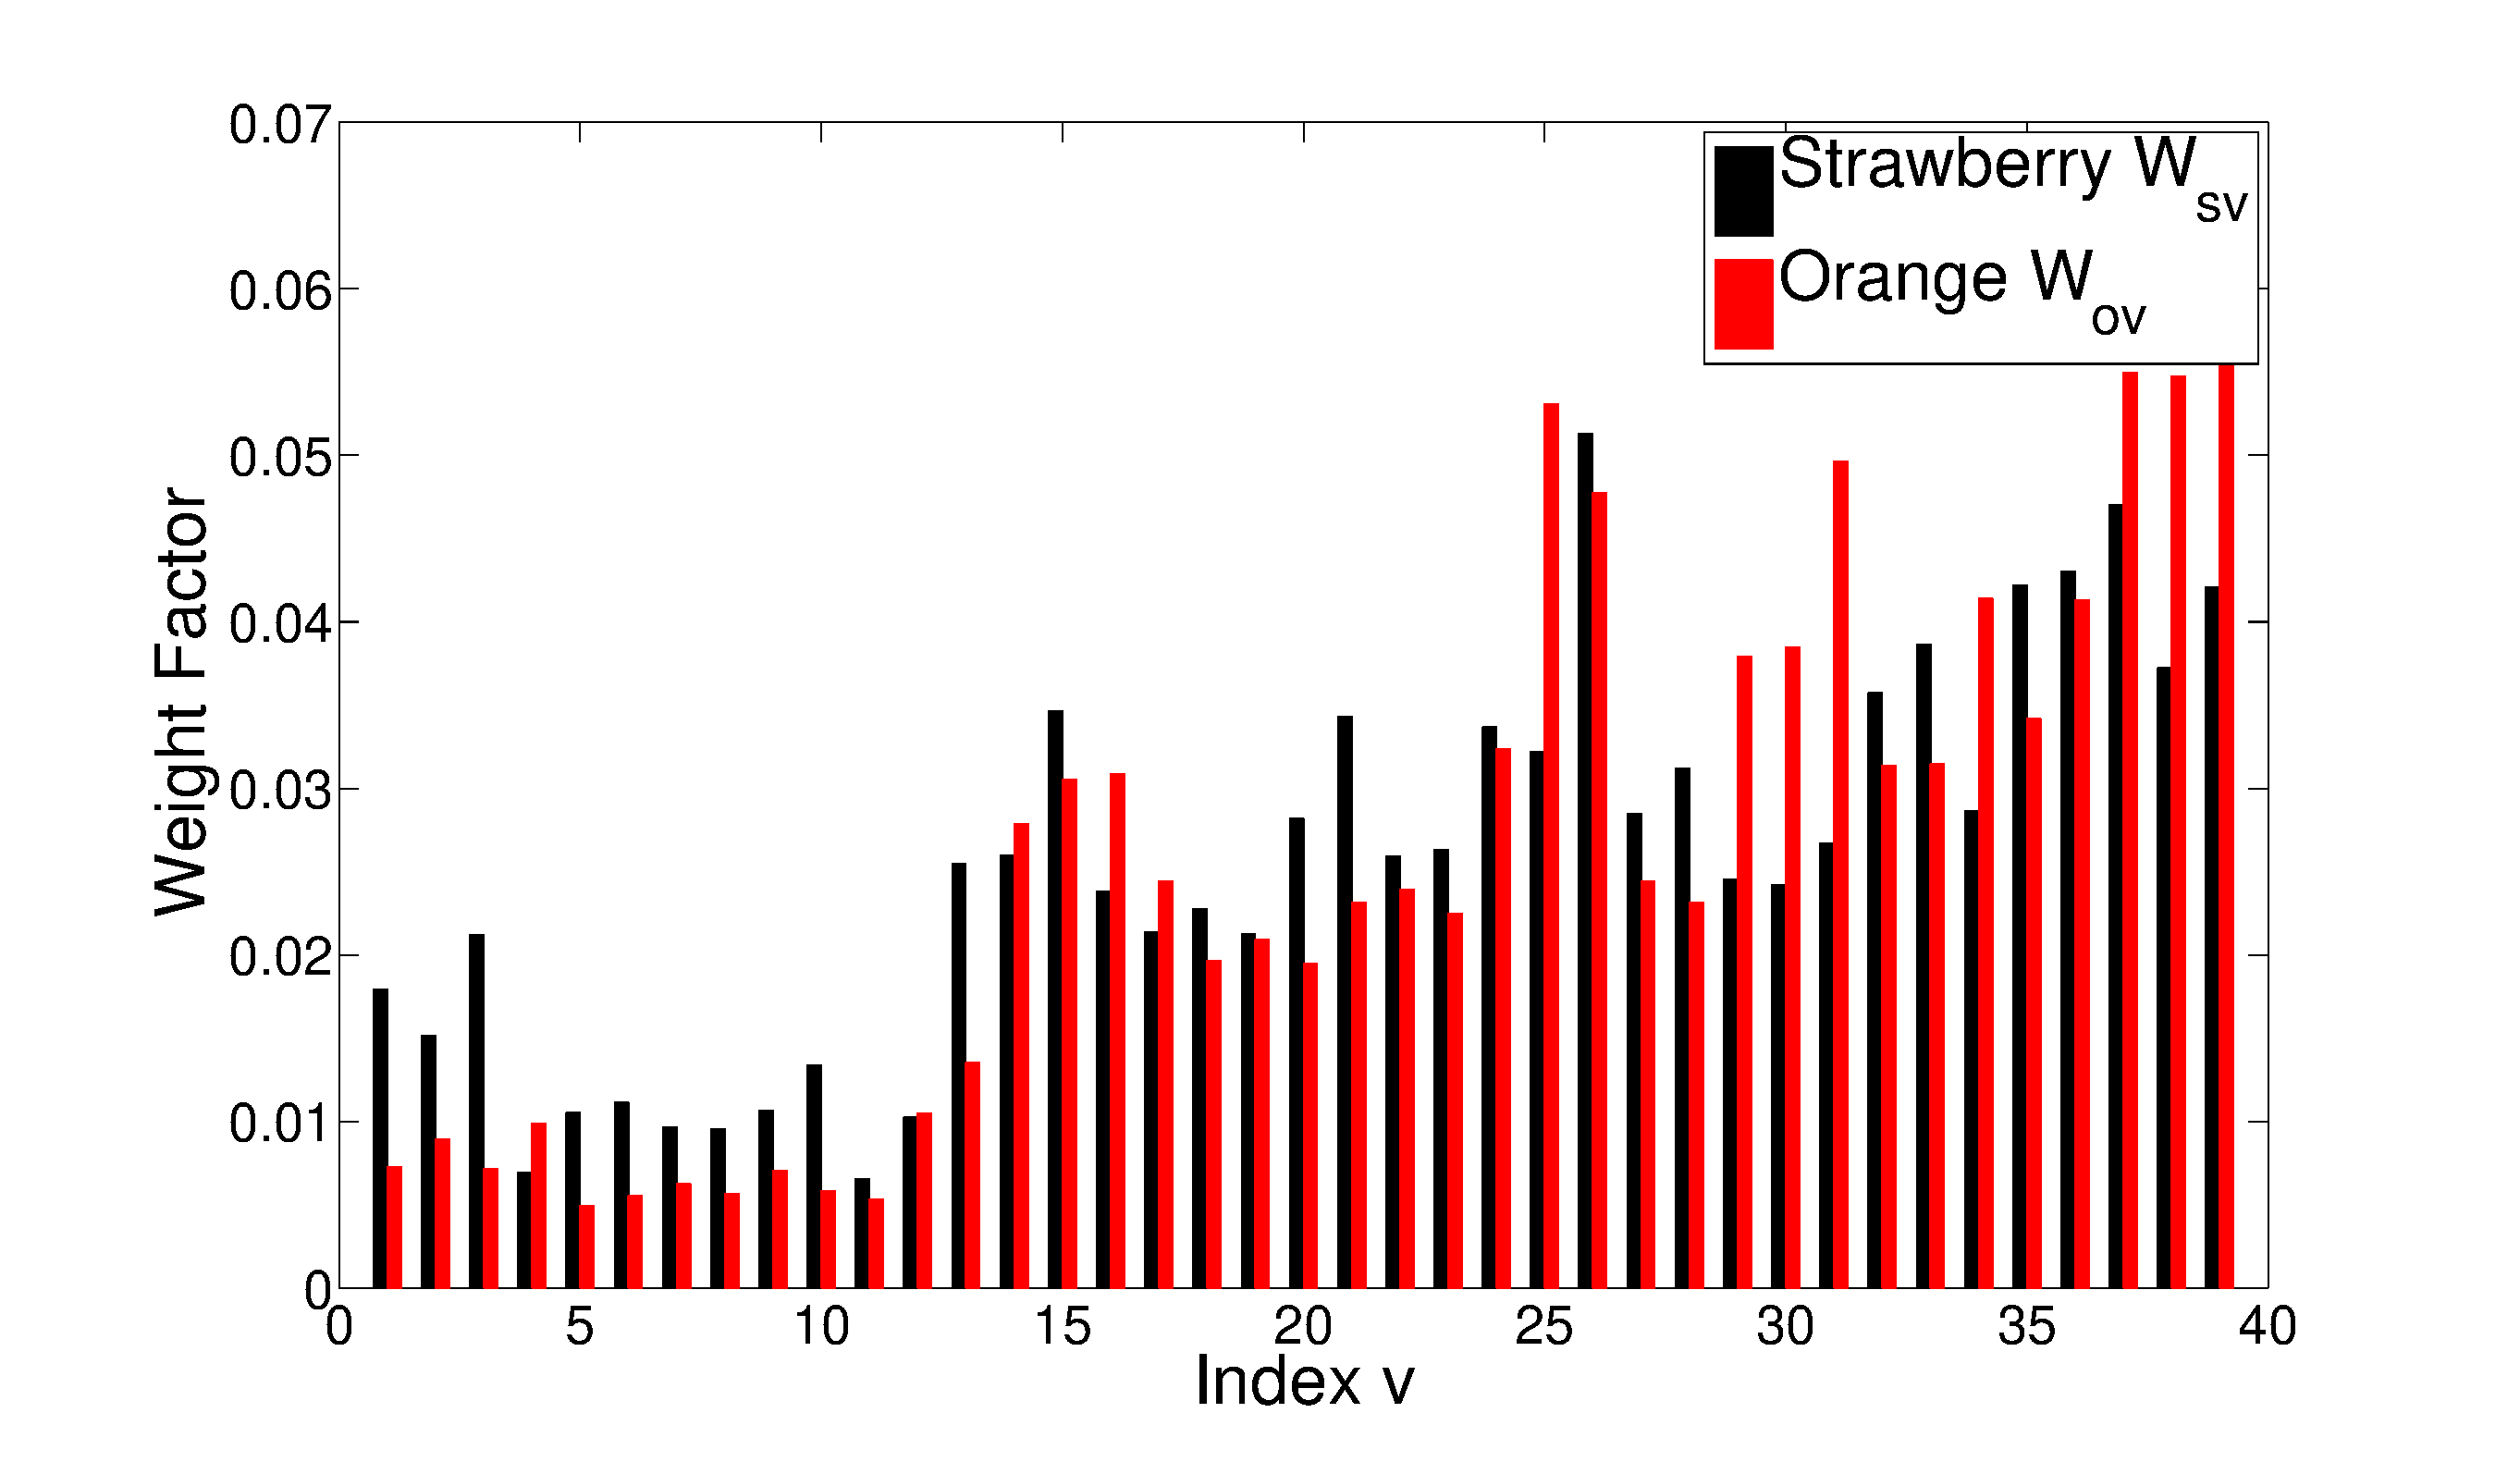
\includegraphics[width=\textwidth]{feature_weights}
  \caption[Feature weights]{The feature weights for strawberry class $F_s$ (black bars) and orange class $F_o$ (red bars)}
  \label{fig:feat_weights}
\end{figure}	
%

The distribution components in $F_p$ with higher values of $w_p$ are weighted higher than the other distributions while performing hypothesis tests. This is discussed in the next section on validation phase of this machine learning algorithm.

\subsection{Validation}
\label{sec:distdes_validation}

\begin{enumerate}
	\item To detect the presence of a target in an image, multiple images of a target are used to compute the feature descriptor.
	
	\item The feature descriptor is then compared against the known classes of feature distributions.
	
	\item If a feature descriptor agrees with a feature distribution for a certain target object class, then the images currently under examination are considered to have sufficient evidence for the presence of an instance from the target object class.
\end{enumerate}

In this object recognition method, a series of height-tagged images of an object specimen is used to perform a binary classification task. In other words, the 13 height-tagged images are used to decide if the object belongs to one of the two classes: $p$ or $q$. In order to achieve this, the histogram signatures (described in Section~\ref{sec:hist_signature}) are computed on each of the 13 height tagged-images available for an object specimen. Since there is no pre-specified label information available, all pixels in the image are used here. The computation performed is identical to the one in \eqref{eqn:hist_signature}, and results in a sequence of 39 histogram signatures $\ddot{\mathcal{H}}^{k}$. 

The next step in the validation procedure is to use \eqref{eqn:hist_signature_dist} and \eqref{eqn:dist_sequence} to compute the distance measure sequences $D^p_k=D(\ddot{\mathcal{H}}^{k}, \bar{\mathcal{H}}^{p})$ and $D^q_k=D(\ddot{\mathcal{H}}^{k}, \bar{\mathcal{H}}^{p})$. The 39-value sequences $D^p_k$ and $D^q_k$ provide information about the \emph{closeness} of the sample specimen $k$ to each of the classes $p$ and $q$. The information in these sequences need to be processed further in order to associate specimen $k$ with either class $p$ or class $q$.

Let us assume that specimen $k$ belongs to class $p$. According to this hypothesis, the $v$-th component of $D^p_k$ should follow the $v$-th distribution of the feature distribution sequence $F_p$. In other words, using \eqref{eqn:conf_interval}, we can state with 95\% \textit{confidence} that condition 
%
\begin{align}
  d^p_{kv} \in C^{0.95}_{F_{pv}}= &[\mu_{pv}-2 \times \sigma_{pv},\, \mu_{pv}+2 \times \sigma_{pv}]
  \label{eqn:conf_interval_validation}
\end{align}
%
is satisfied. If we call this hypothesis test $h^p_{kv}$, then passing of this hypothesis test
%
\begin{align}
 h^p_{kv} = &
 \begin{cases}
    1	&	d^p_{kv} \in C^{0.95}_{F_{pv}}\\
    0	&	otherwise
 \end{cases} \label{eqn:hypothesis_test}
\end{align}
%
meaning $(h^p_{kv}=1)$, determines that specimen $k$ belongs to class $p$.

There are 39 such hypothesis tests, $h^p_{k1}, h^p_{k2},\ldots, h^p_{k39}$ that can be performed to determine if specimen $k$ belongs to class $p$.
The importance of each of these hypothesis tests for associating specimen $k$ with class $p$ is determined by the corresponding weight $w_{pv}$. The information available in the form of hypothesis tests, along with their associated weights, is combined in to a single numeric metric or \emph{class confidence} 
%
\begin{align} \label{eqn:numeric_class_metric}
 H^p_k=\sum_{v=1}^{39} h^p_{kv} w_{pv} 
\end{align}
%
that measures the confidence in specimen $k$ belonging to class $p$.

It is important to note that based on ~\eqref{eqn:feat_wt_norm}, it follows that $H^p_c\in[0,1]$. If $H^p_k=1$, then we can say with high confidence that specimen $k$ belongs to class $p$. Alternatively, $H^p_k=0$ suggests that its unlikely that specimen $k$ belongs to class $p$. A similar metric $H^q_k$ is computed to determine confidence in the assertion that
specimen $k$ belongs to class $q$. Finally, the binary classification task that classifies specimen $k$ into class $p$ or class $q$ is decided based on the magnitude of $H^p_k$ and $H^q_k$:
%
\begin{align}	\label{eqn:binary_classification}
 H^p_k > H^q_k	&{} &\text{specimen}\, k \in \text{class}\, p\nonumber\\
 H^p_k < H^q_k	&{} &\text{specimen}\, k \in \text{class}\, q\nonumber\\
 H^p_k = H^q_k	&{} &\text{Undetermined}
\end{align}


%================================================================================================================
\section{Results}
\begin{enumerate}
	\item The data collected for this experiment consisted of 11 specimens of oranges and 13 specimens of strawberries each from 13 different heights in an underwater settings.
	
	\item The feature distribution for orange and strawberry is shown in the figure.
	
	\item A leave-1-out cross-validation was performed to validate the developed machine learning technique.
	
	\item The feature descriptor plot for each specimen is compared against the feature distributions of the strawberry and orange class.
\end{enumerate}

The data collected during the experiments involve images from 11 specimens of both orange class and strawberry class. Data on each specimen included images taken from 13 different heights, starting at 32 inches from the ground, down to 8 inches, away from the ground. The imaging experiment was conducted in a test tank filled with water using the imaging rig shown in Figure~\ref{fig:im_rig}. More details of the data collection process can be found in Section~\ref{sec:distdes_data_collection}. Following the data collection process, the feature distribution sequence $F_{s}$ for strawberry class, and $F_{o}$  for orange class, are computed using the procedure discussed in Section~\ref{sec:distdes_feature_distr}; the results are shown in Figure~\ref{fig:feat_distr}.

As part of an initial validation step, both learning and testing is done on the entire dataset of 22 specimens. The learning procedure
results in feature distributions for strawberry and orange which are are shown in Figure~\ref{fig:feat_distr}. Then each specimen is evaluated against both strawberry and orange feature distributions as described in Section~\ref{sec:distdes_validation}, to get distance metric sequences $D^s_k$ and $D^o_k$. The 11 strawberry specimens are checked against the strawberry and orange feature distribution sequences $F_{s}$ and $F_{o}$; see Figure~\ref{fig:feat_results_strawberry_test}. The solid blue line in Figure~\ref{fig:feat_results_strawberry_test_strawberry_learn} along with the gray band is an alternate representation of strawberry feature distribution sequence $F_{s}$ (shown in Figure~\ref{fig:feat_distr_strawberry}). The solid blue line represents the mean of the feature distributions along with the 95\% confidence region shown as a gray band. The additional difference in this representation of $F_s$ is that the indices $v$ are now arranged in the decreasing order according to their importance, with the 
latter inferred by the strawberry feature weights $W_s$. In other words, the first distribution in Figure~\ref{fig:feat_results_strawberry_test_strawberry_learn} corresponds to the feature distribution with the highest feature weight in $W_{s}$, and the 
last distribution is the 
feature distribution with the lowest feature weight in $W_{s}$. 
The colored lines in Figure~\ref{fig:feat_results_strawberry_test_strawberry_learn}, represent the distance metric sequences $D^s_k$ of the 11 strawberry specimens. 
All the 11 colored lines lie inside the confidence region indicating that the 
distance metric sequence of strawberry specimens are in agreement with the strawberry-class distribution sequence $F_{s}$.
In Figure~\ref{fig:feat_results_strawberry_test_orange_learn}, we compare the same 11 strawberry specimens against the orange-class distribution sequence $F_{o}$. Here the orange-class distribution sequence $F_{o}$ is again represented by the combination of solid blue line with a gray band around it. However, since only strawberry specimens are being considered here, the sequence of feature distributions are again arranged in the decreasing order of importance as captured in the strawberry feature weights $W_s$. The colored lines here represent the distance metric sequence $D^o_k$ values for the 11 strawberry specimens.
In contrast with Figure~\ref{fig:feat_results_strawberry_test_orange_learn}, the colored lines are not in agreement with the confidence region of the orange-class feature distribution sequence $F_{o}$.
In Figure~\ref{fig:feat_results_strawberry_test_strawberry_learn} we can observe that the strawberry distance metric sequence $D^s_k$ almost always lies inside the confidence region while compared with Figure~\ref{fig:feat_results_strawberry_test_orange_learn} where the $D^o_k$ often lie outside the confidence region. This is a clear indicator of strawberry specimens matching better with the strawberry-class feature distribution $F_s$ compared to orange-class feature distribution $F_o$. On similar lines, the 11 orange specimens are compared against the orange-class feature distribution $F_{o}$ in Figure~\ref{fig:feat_results_orange_test_orange_learn} and also compared against strawberry-class feature distribution $F_{s}$ in Figure~\ref{fig:feat_results_orange_test_strawberry_learn}. The observations show that the orange specimens match closer with orange feature distribution sequence $F_{o}$ rather than the strawberry feature distribution sequence $F_{s}$. This again reinforces that the distance metric 
values of both orange and strawberry specimens agree with their corresponding class distribution sequences.

%
\begin{figure*}
  %\vskip -12pt
  \centering
  \begin{subfigure}[]{0.6\textwidth}
      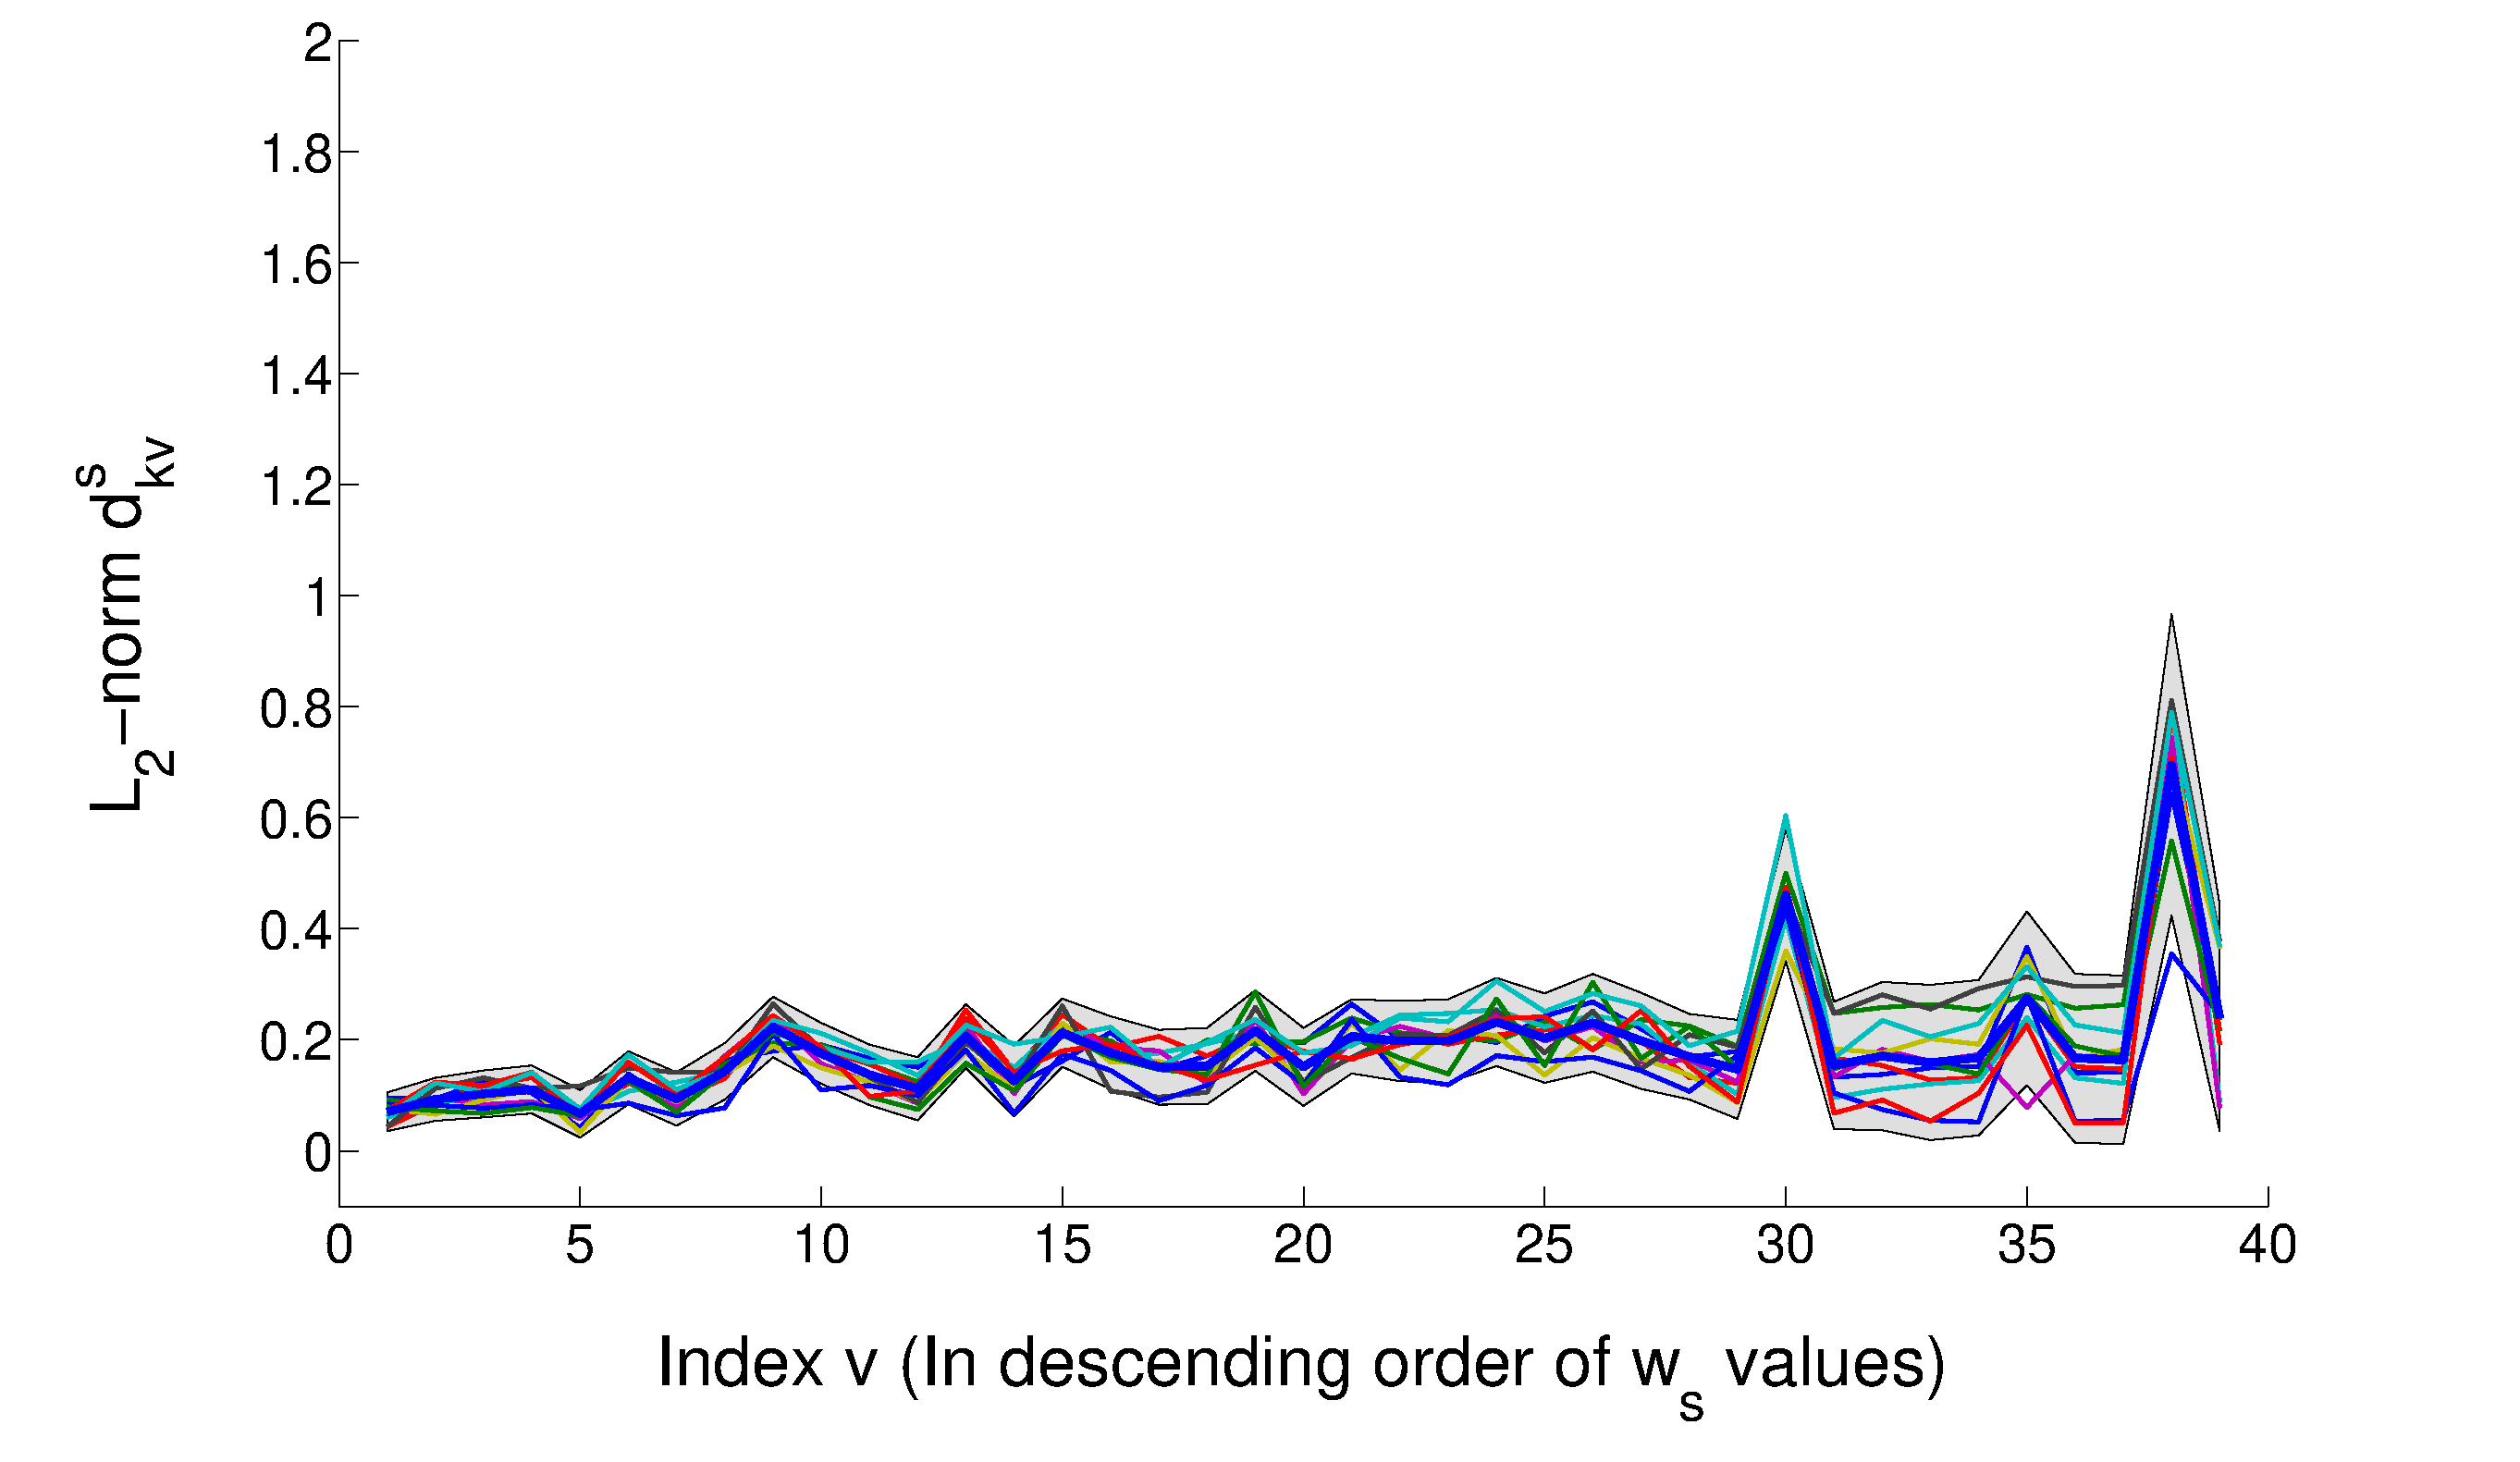
\includegraphics[width=\textwidth]{validation_strawberry_testset_strawberry_learnset}
      \caption{Strawberry specimens evaluated against strawberry feature distribution sequence $F_s$}
      \label{fig:feat_results_strawberry_test_strawberry_learn}
  \end{subfigure}
  \begin{subfigure}[]{0.6\textwidth}
      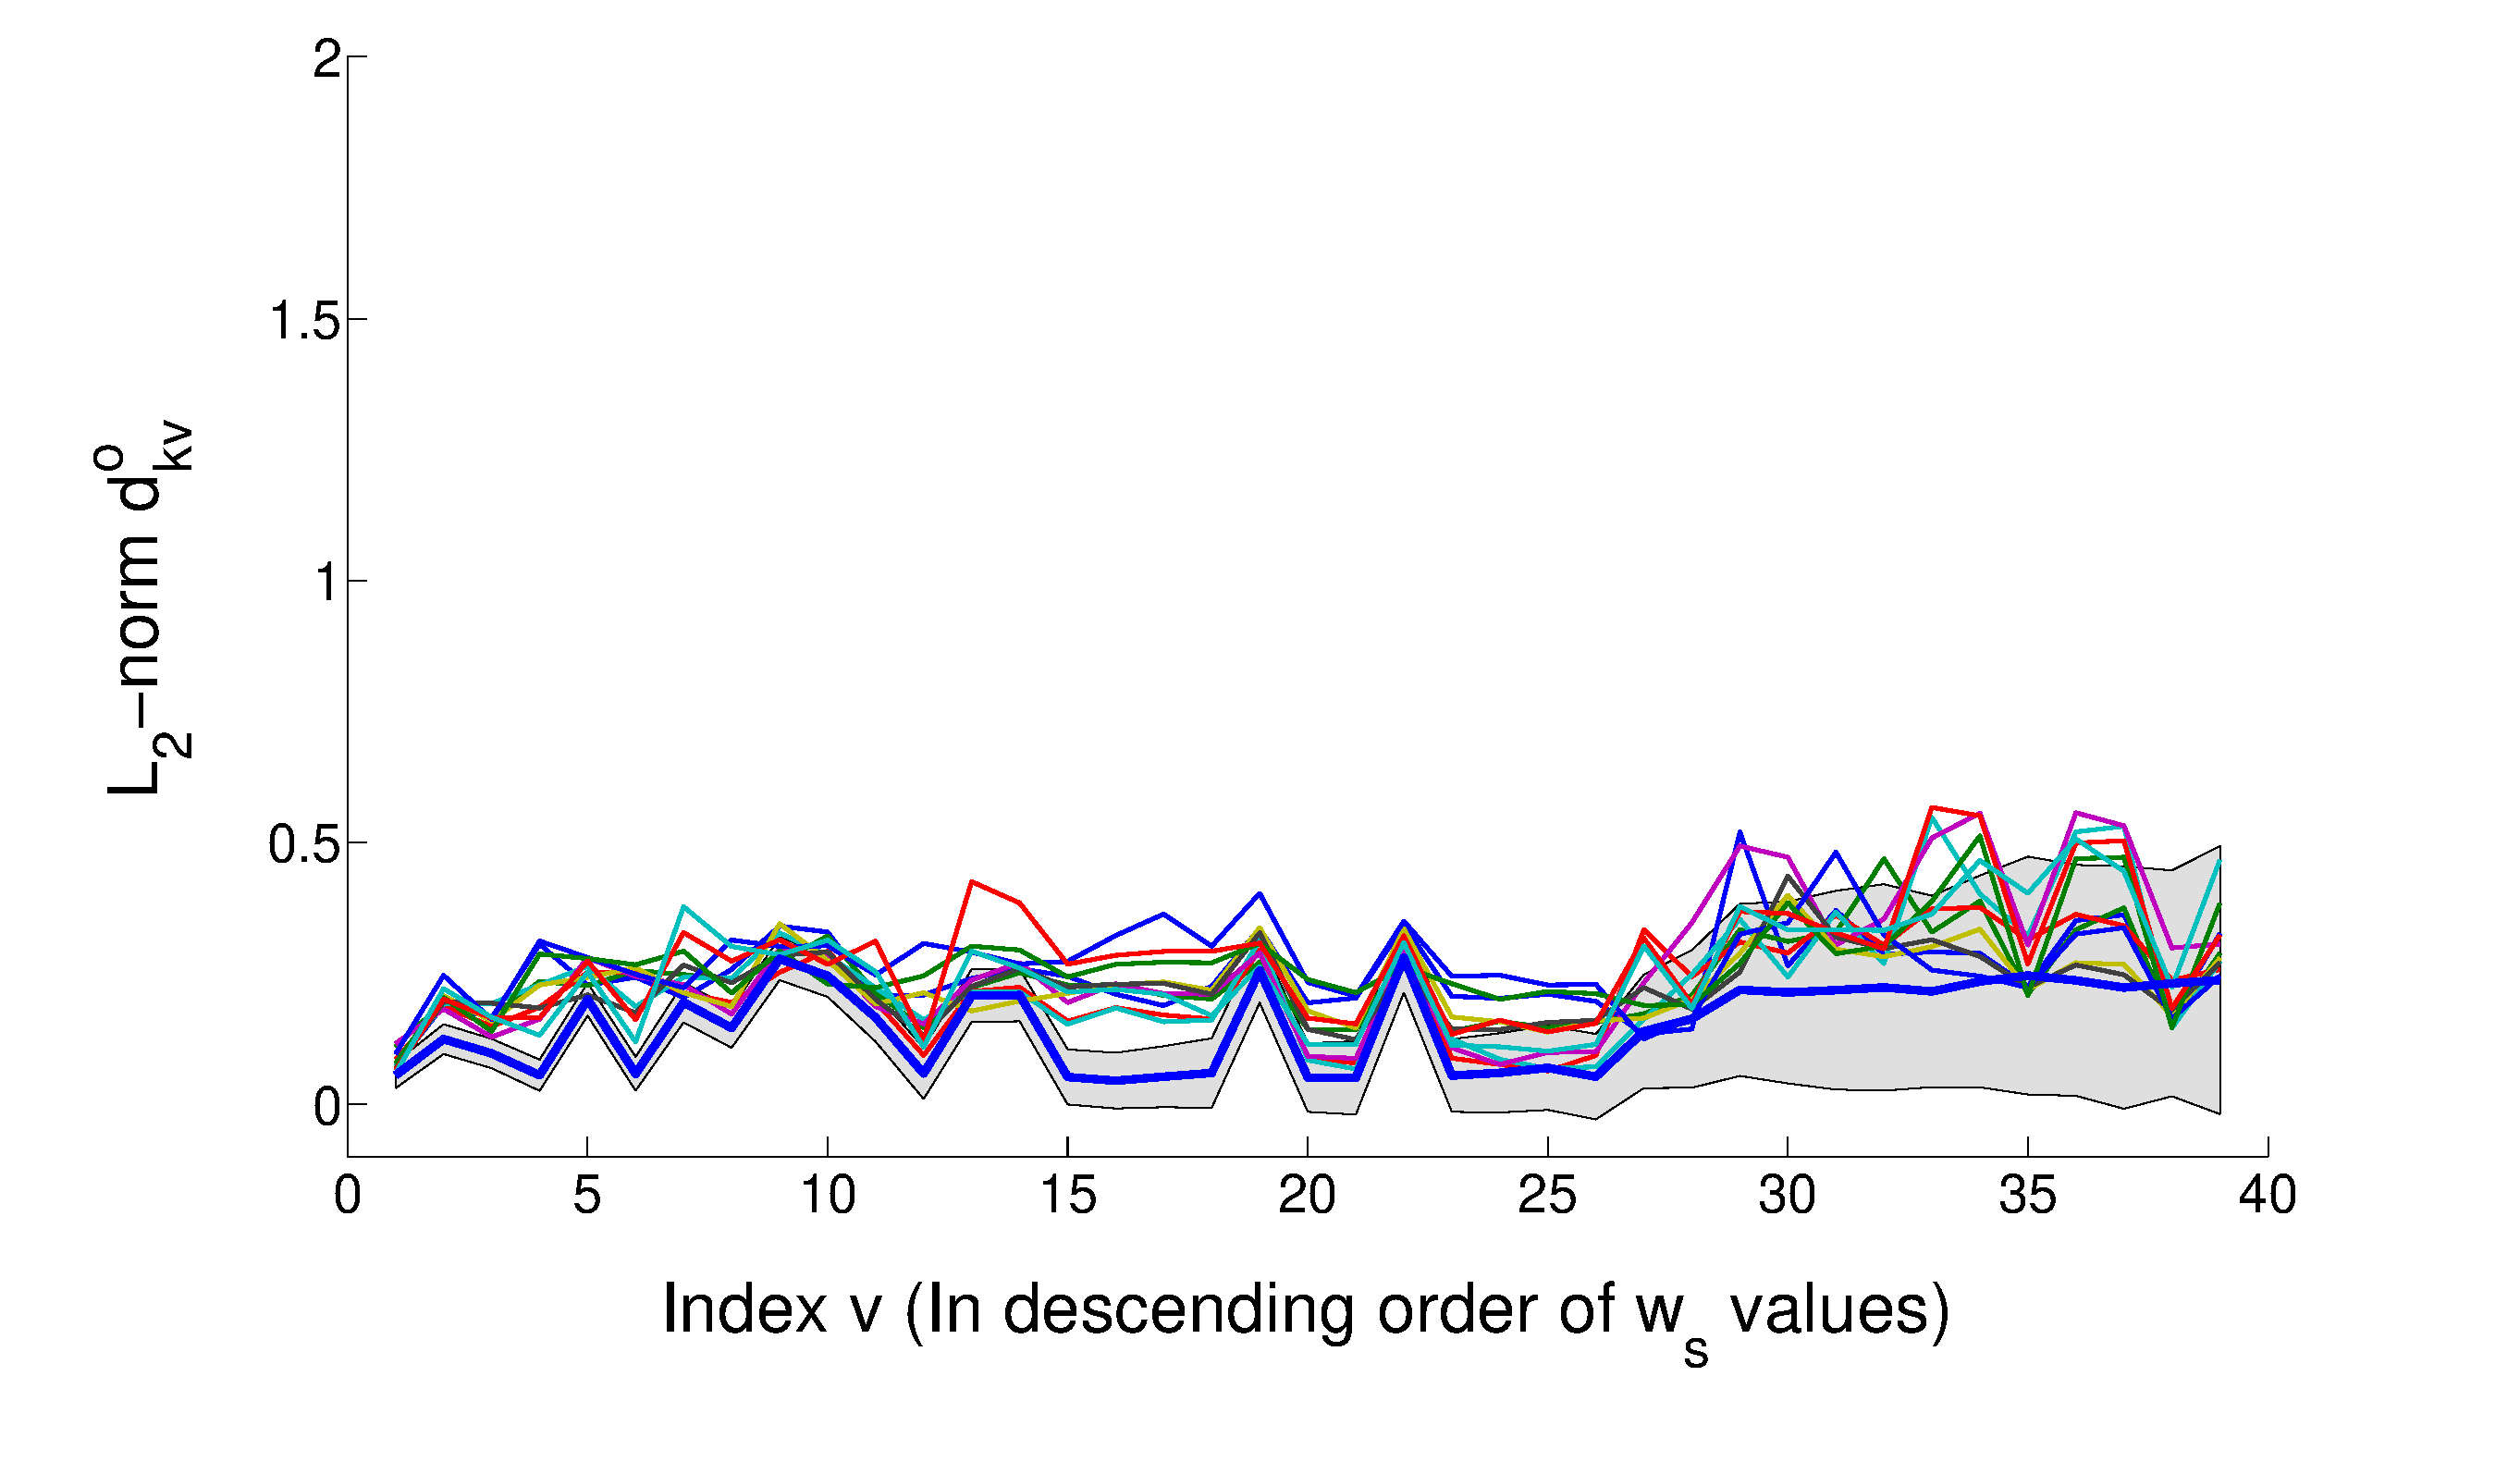
\includegraphics[width=\textwidth]{validation_strawberry_testset_orange_learnset}
      \caption{Strawberry specimens evaluated against orange feature distribution sequence $F_o$}
      \label{fig:feat_results_strawberry_test_orange_learn}
  \end{subfigure}
\caption[Strawberry specimen validation results]{Validation results obtained 
while evaluating strawberry specimens against 
strawberry-class feature distribution sequence $F_s$ (\subref{fig:feat_results_strawberry_test_strawberry_learn}) and against the
orange-class feature distribution sequence $F_o$ 
(\subref{fig:feat_results_strawberry_test_orange_learn}). The strawberry-class feature distribution sequence $F_s$ is shown in (\subref{fig:feat_results_strawberry_test_strawberry_learn}): mean is represented as the solid blue line and the 95\% confidence region is shown as a gray band around the mean. The sequence of feature distributions indexed by $v$ is arranged in the decreasing order of importance as captured in the strawberry feature weights $W_s$. The colored lines in (\subref{fig:feat_results_strawberry_test_strawberry_learn}), represent the distance metric sequence $D^s_k$ of the 11 strawberry specimens. All the 11 colored lines in (\subref{fig:feat_results_strawberry_test_strawberry_learn}) mostly lie inside the confidence region indicating that the distance metric values of strawberry specimens are in agreement with the strawberry-class distribution sequence $F_s$.
In (\subref{fig:feat_results_strawberry_test_orange_learn}), the same 11 strawberry specimens are checked against the orange-class feature distribution sequence $F_o$. In this case, the solid blue line and gray confidence region are representative of the orange-class feature distribution sequence $F_o$. However, since only strawberry specimens are considered here, the sequence of feature distributions are again arranged in the decreasing order of importance as captured in the strawberry feature weights $W_s$. In contrast to (\subref{fig:feat_results_strawberry_test_strawberry_learn}), the colored lines in (\subref{fig:feat_results_strawberry_test_orange_learn}) do not agree with the orange-class feature distribution sequence $F_o$. This signifies that the strawberry specimens only agree with the strawberry feature distribution sequence $F_s$ and not with orange distribution sequence $F_o$.}
\label{fig:feat_results_strawberry_test}
\end{figure*}	
%
\begin{figure*}
  \vskip -12pt
  \centering
  \begin{subfigure}[]{0.6\textwidth}
      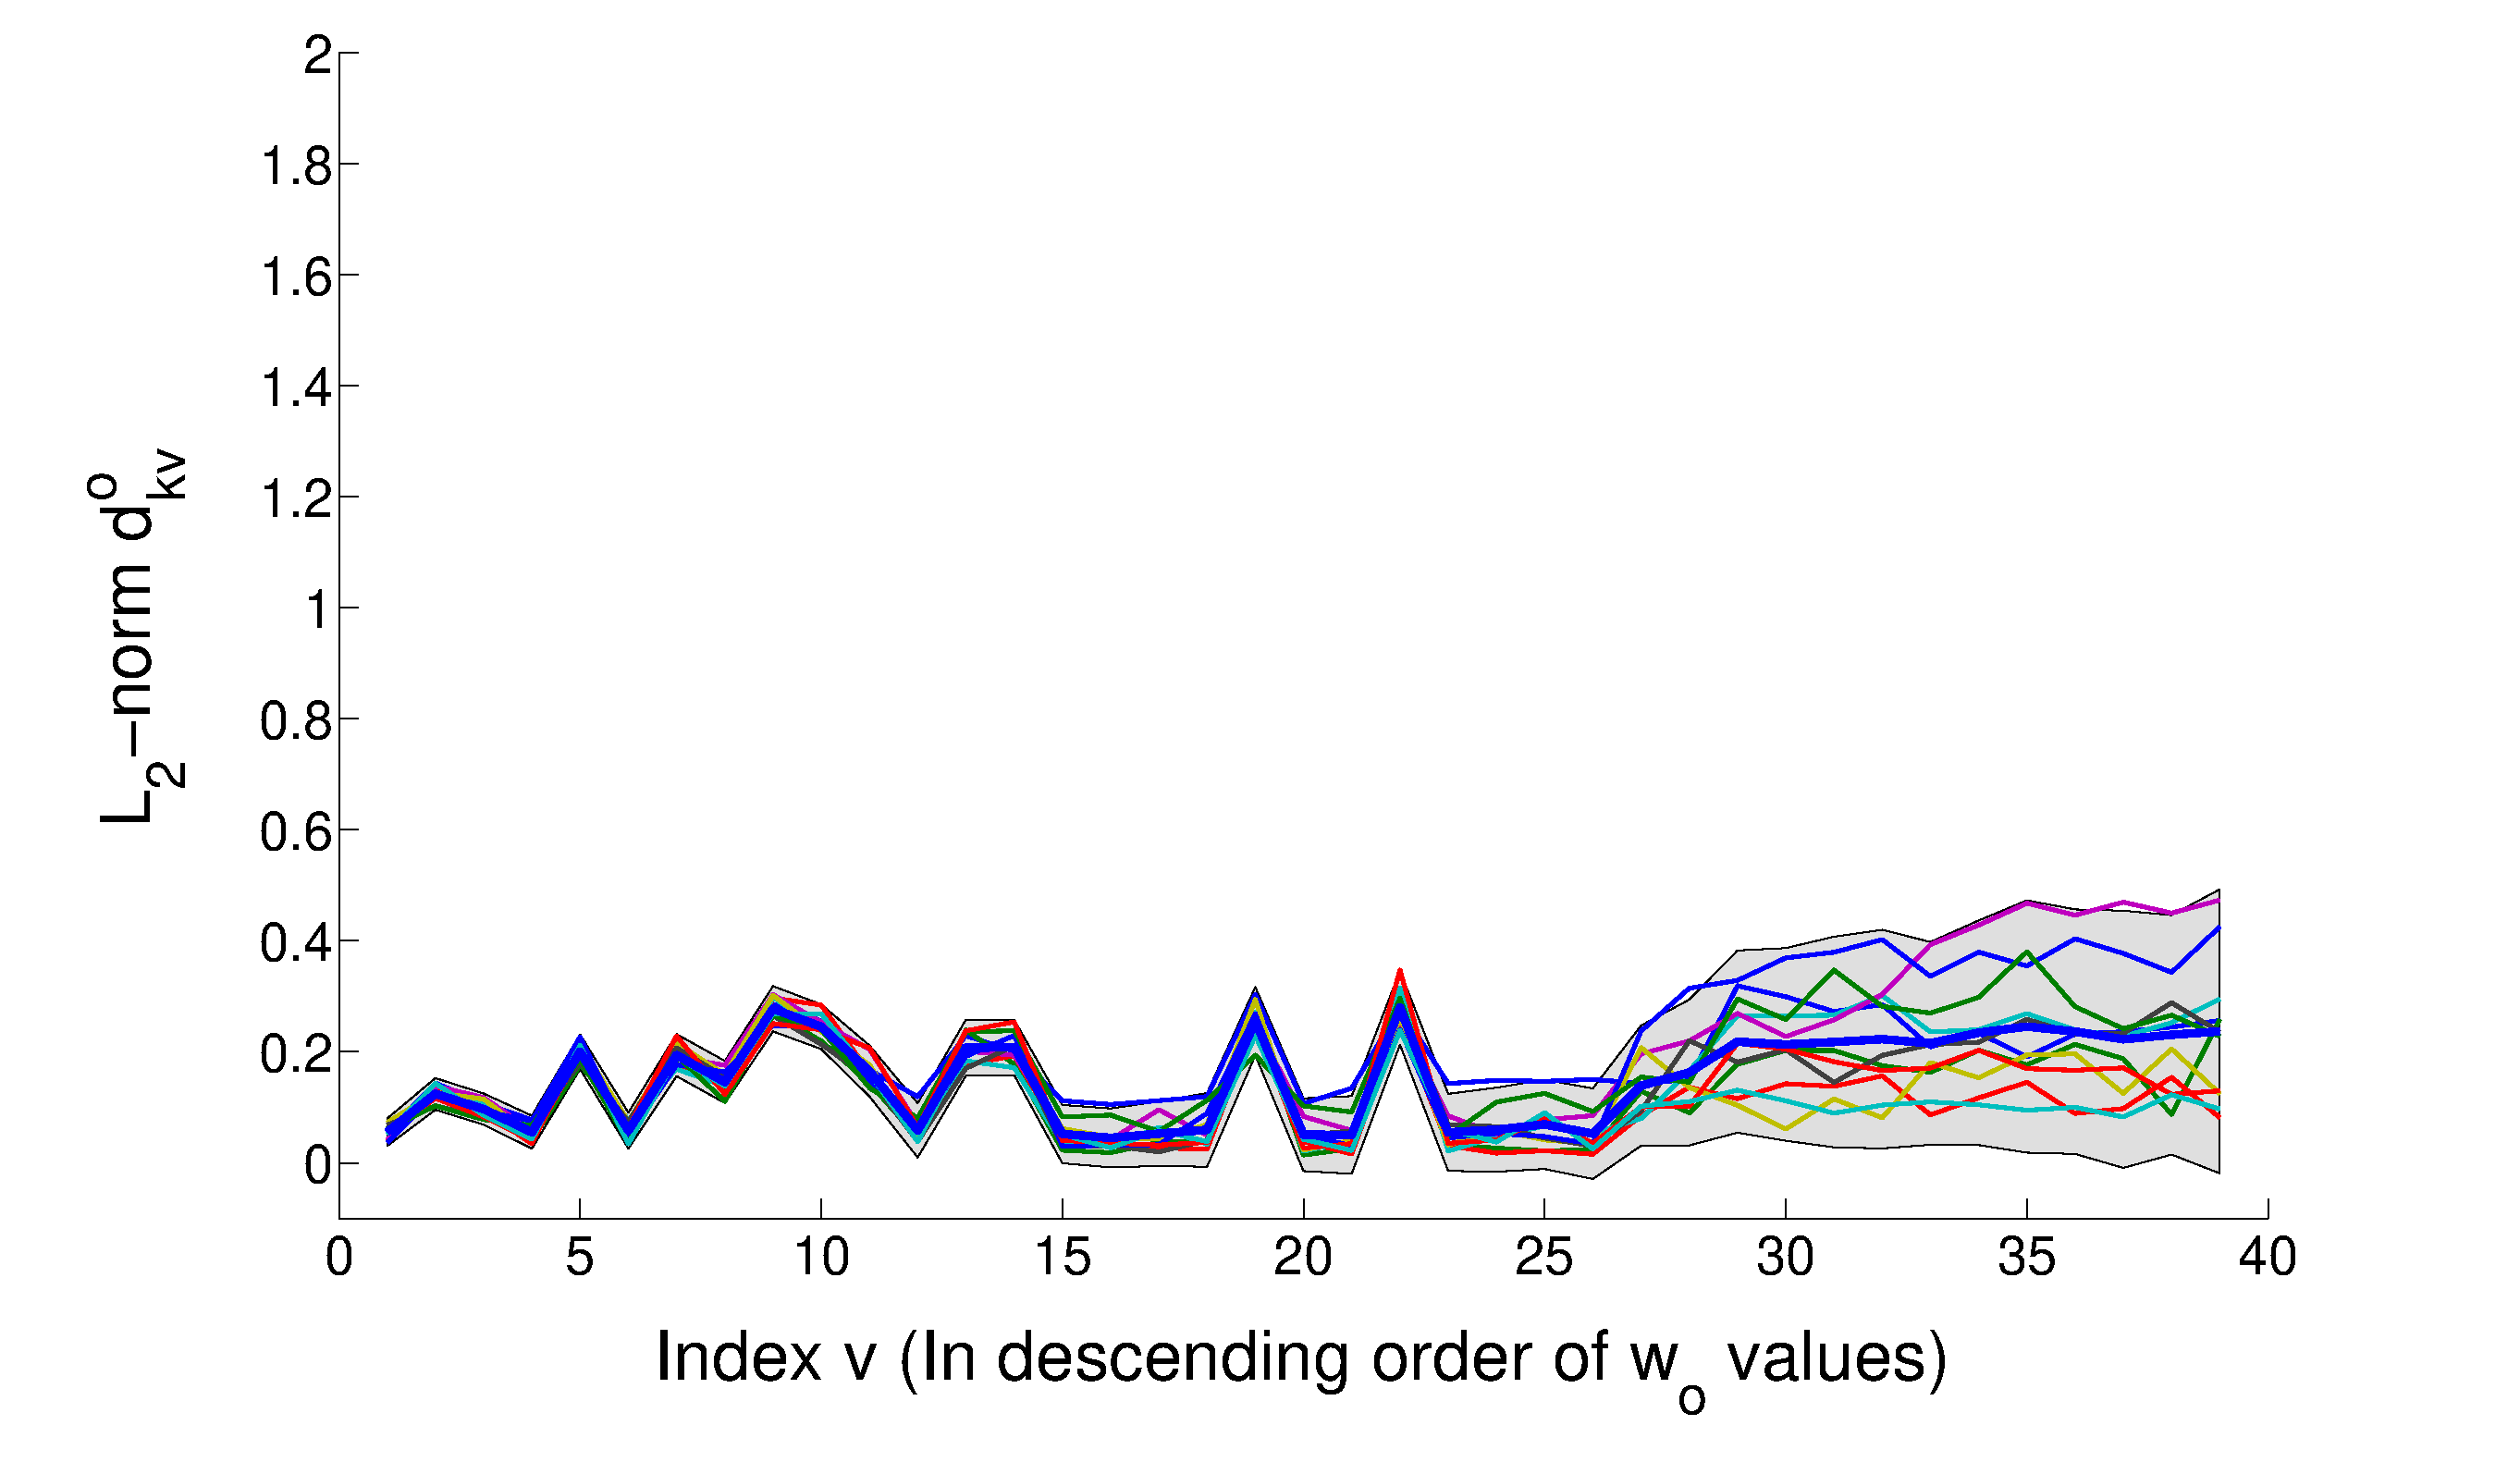
\includegraphics[width=\textwidth]{validation_orange_testset_orange_learnset}
      \caption{Orange specimens evaluated against orange feature distribution sequence $F_o$}
      \label{fig:feat_results_orange_test_orange_learn}
  \end{subfigure}
  \begin{subfigure}[]{0.6\textwidth}
      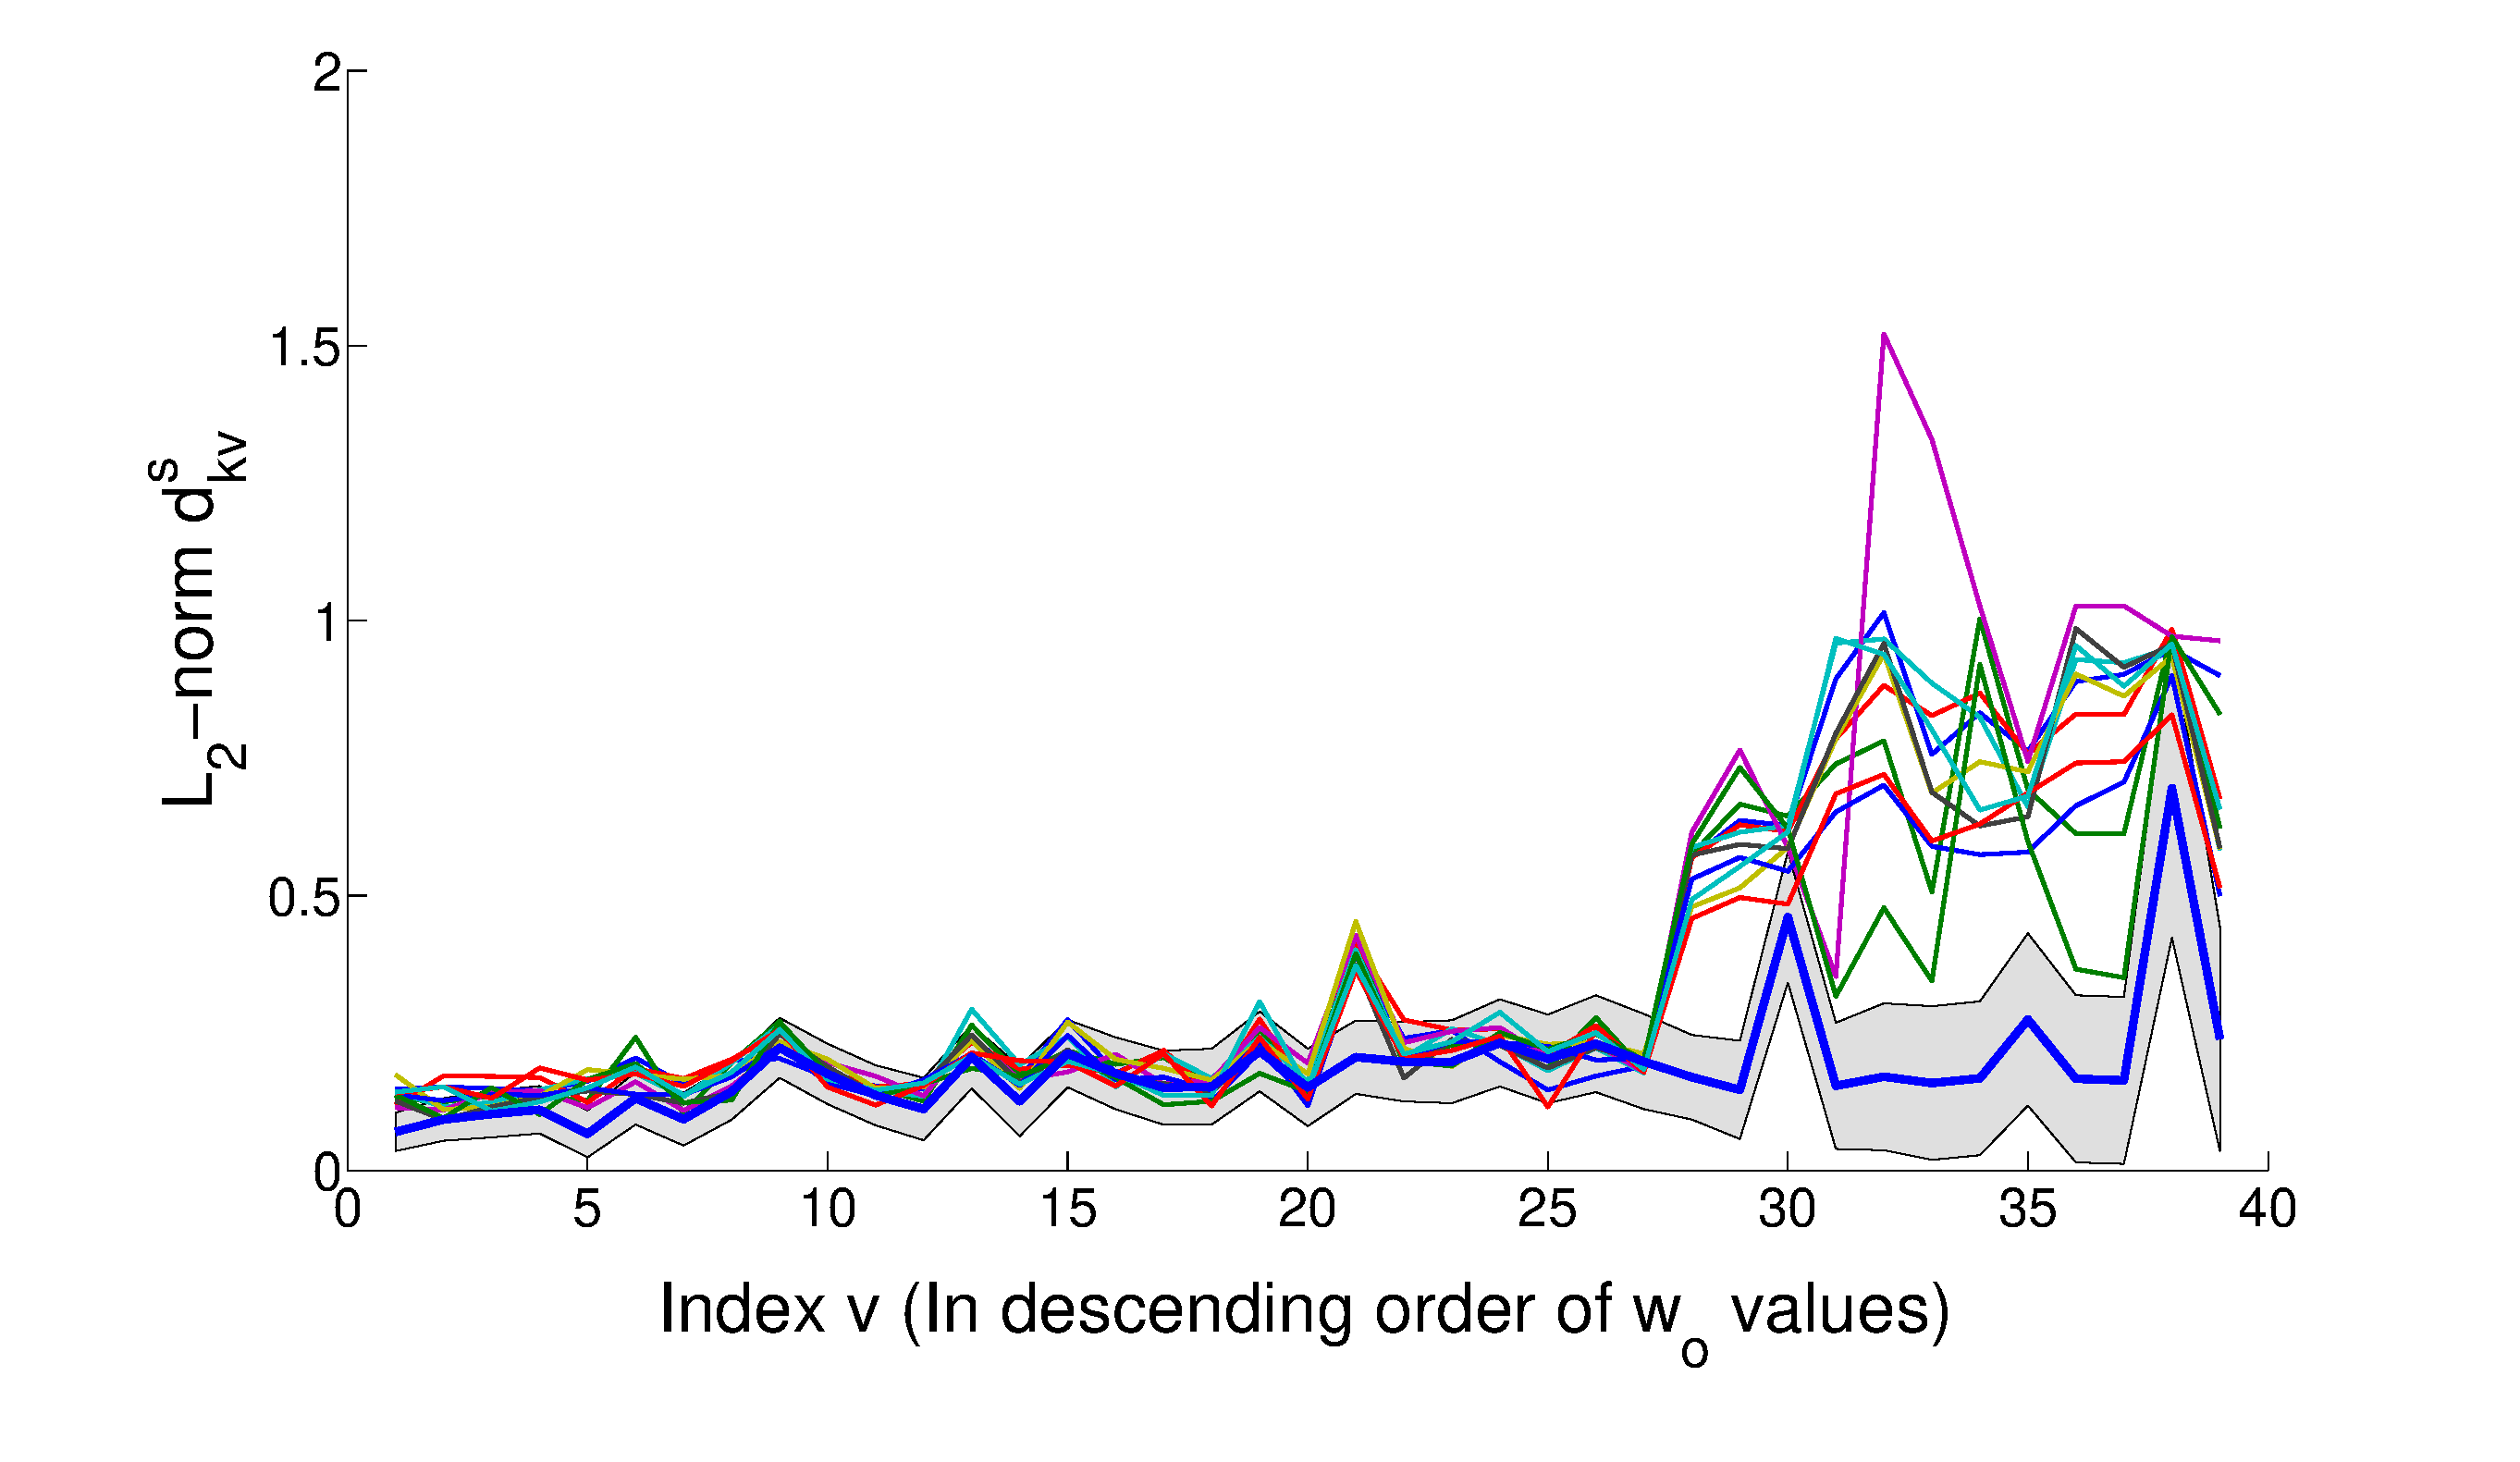
\includegraphics[width=\textwidth]{validation_orange_testset_strawberry_learnset}
      \caption{Orange specimens evaluated against strawberry feature distribution sequence $F_s$}
      \label{fig:feat_results_orange_test_strawberry_learn}
  \end{subfigure}
\caption[Orange specimen validation results]{Similar to Figure~\ref{fig:feat_results_strawberry_test} that show the validation results for strawberry specimens, this figure shows the validation results for orange specimens. Testing of orange specimens against 
orange-class feature distribution sequence $F_o$ is shown in 
(\subref{fig:feat_results_orange_test_orange_learn}), and testing against the
strawberry-class feature distribution sequence $F_s$ is shown in
(\subref{fig:feat_results_orange_test_strawberry_learn}). 
The orange-class feature distribution sequence $F_o$ is shown in (\subref{fig:feat_results_strawberry_test_strawberry_learn}): mean is represented as the solid blue line and the 95\% confidence region is shown as a gray band around the mean. The sequence of feature distributions indexed by $v$ is arranged in the decreasing order of importance as captured in the orange feature weights $W_o$. The colored lines in (\subref{fig:feat_results_orange_test_orange_learn}), represent the distance metric sequence $D^o_k$ of the 11 orange specimens. All the 11 colored lines in (\subref{fig:feat_results_orange_test_orange_learn}) mostly lie inside the confidence region indicating that the distance metric values of orange specimens are in agreement with the orange-class distribution sequence $F_o$.
In (\subref{fig:feat_results_orange_test_strawberry_learn}), the same 11 strawberry specimens are considered against the strawberry-class feature distribution sequence $F_s$. In this case, the solid blue line and gray confidence region are representative of the strawberry-class feature distribution sequence $F_s$. However, since only orange specimens are evaluated here, the sequence of feature distributions are again arranged in the decreasing order of importance as captured in the orange feature weights $W_o$. In contrast to (\subref{fig:feat_results_orange_test_orange_learn}), the colored lines in (\subref{fig:feat_results_orange_test_strawberry_learn}) do not agree with the strawberry-class feature distribution sequence $F_s$. This signifies that the orange specimens only agree with the orange feature distribution sequence $F_o$ and not with strawberry distribution sequence $F_s$.}
\label{fig:feat_results_orange_test}
\end{figure*}	
%

A more concrete validation of this machine learning approach is by computing the \emph{class confidence} $H^s_k$ and $H^o_k$ of each specimen, and deciding on the class of the specimen as described in Section~\ref{sec:distdes_validation}. One thing to note here is that the class confidence measure requires the feature distribution sequences of the strawberry and orange classes to be computed. The feature distribution sequences are generated from the learning set; the learning set contains the specimen we are currently trying to recognize. It is a general rule to separate the learning and testing datasets before validating a machine learning algorithm. In this case, since the dataset consists of only 22 specimens, a leave-one-out cross-validation \cite{alpaydin} was implemented.\footnote{Leave-one-out cross-validation is used in cases where the number of specimens available is very small. In such cases, one does not have the luxury of splitting the available labeled dataset into 
learning and testing sets. Therefore, in leave-one-out cross-validation, during each iteration one 
specimen is chosen as the testing set and the all other specimens are chosen as the learning set. Thus the learning procedure is repeated in each iteration, without adding the instance that is being tested to the learning set.} The class confidence values $H^s_k$ and $H^o_k$ of the 11 strawberry specimens are shown as black and red bars respectively in Figure~\ref{fig:results_strawberry}. It is clear that the black bars are taller than the red bars in all cases. According to the hypothesis test in force (see \eqref{eqn:hypothesis_test}), this implies that that all strawberry specimens are classified correctly. The same can be said for the orange specimens. As seen in Figure~\ref{fig:results_orange}: all the red bars are taller than the back bars. Therefore, all orange specimens are also classified correctly.

%
\begin{figure*}
  \centering
  \begin{subfigure}[]{0.7\textwidth}
      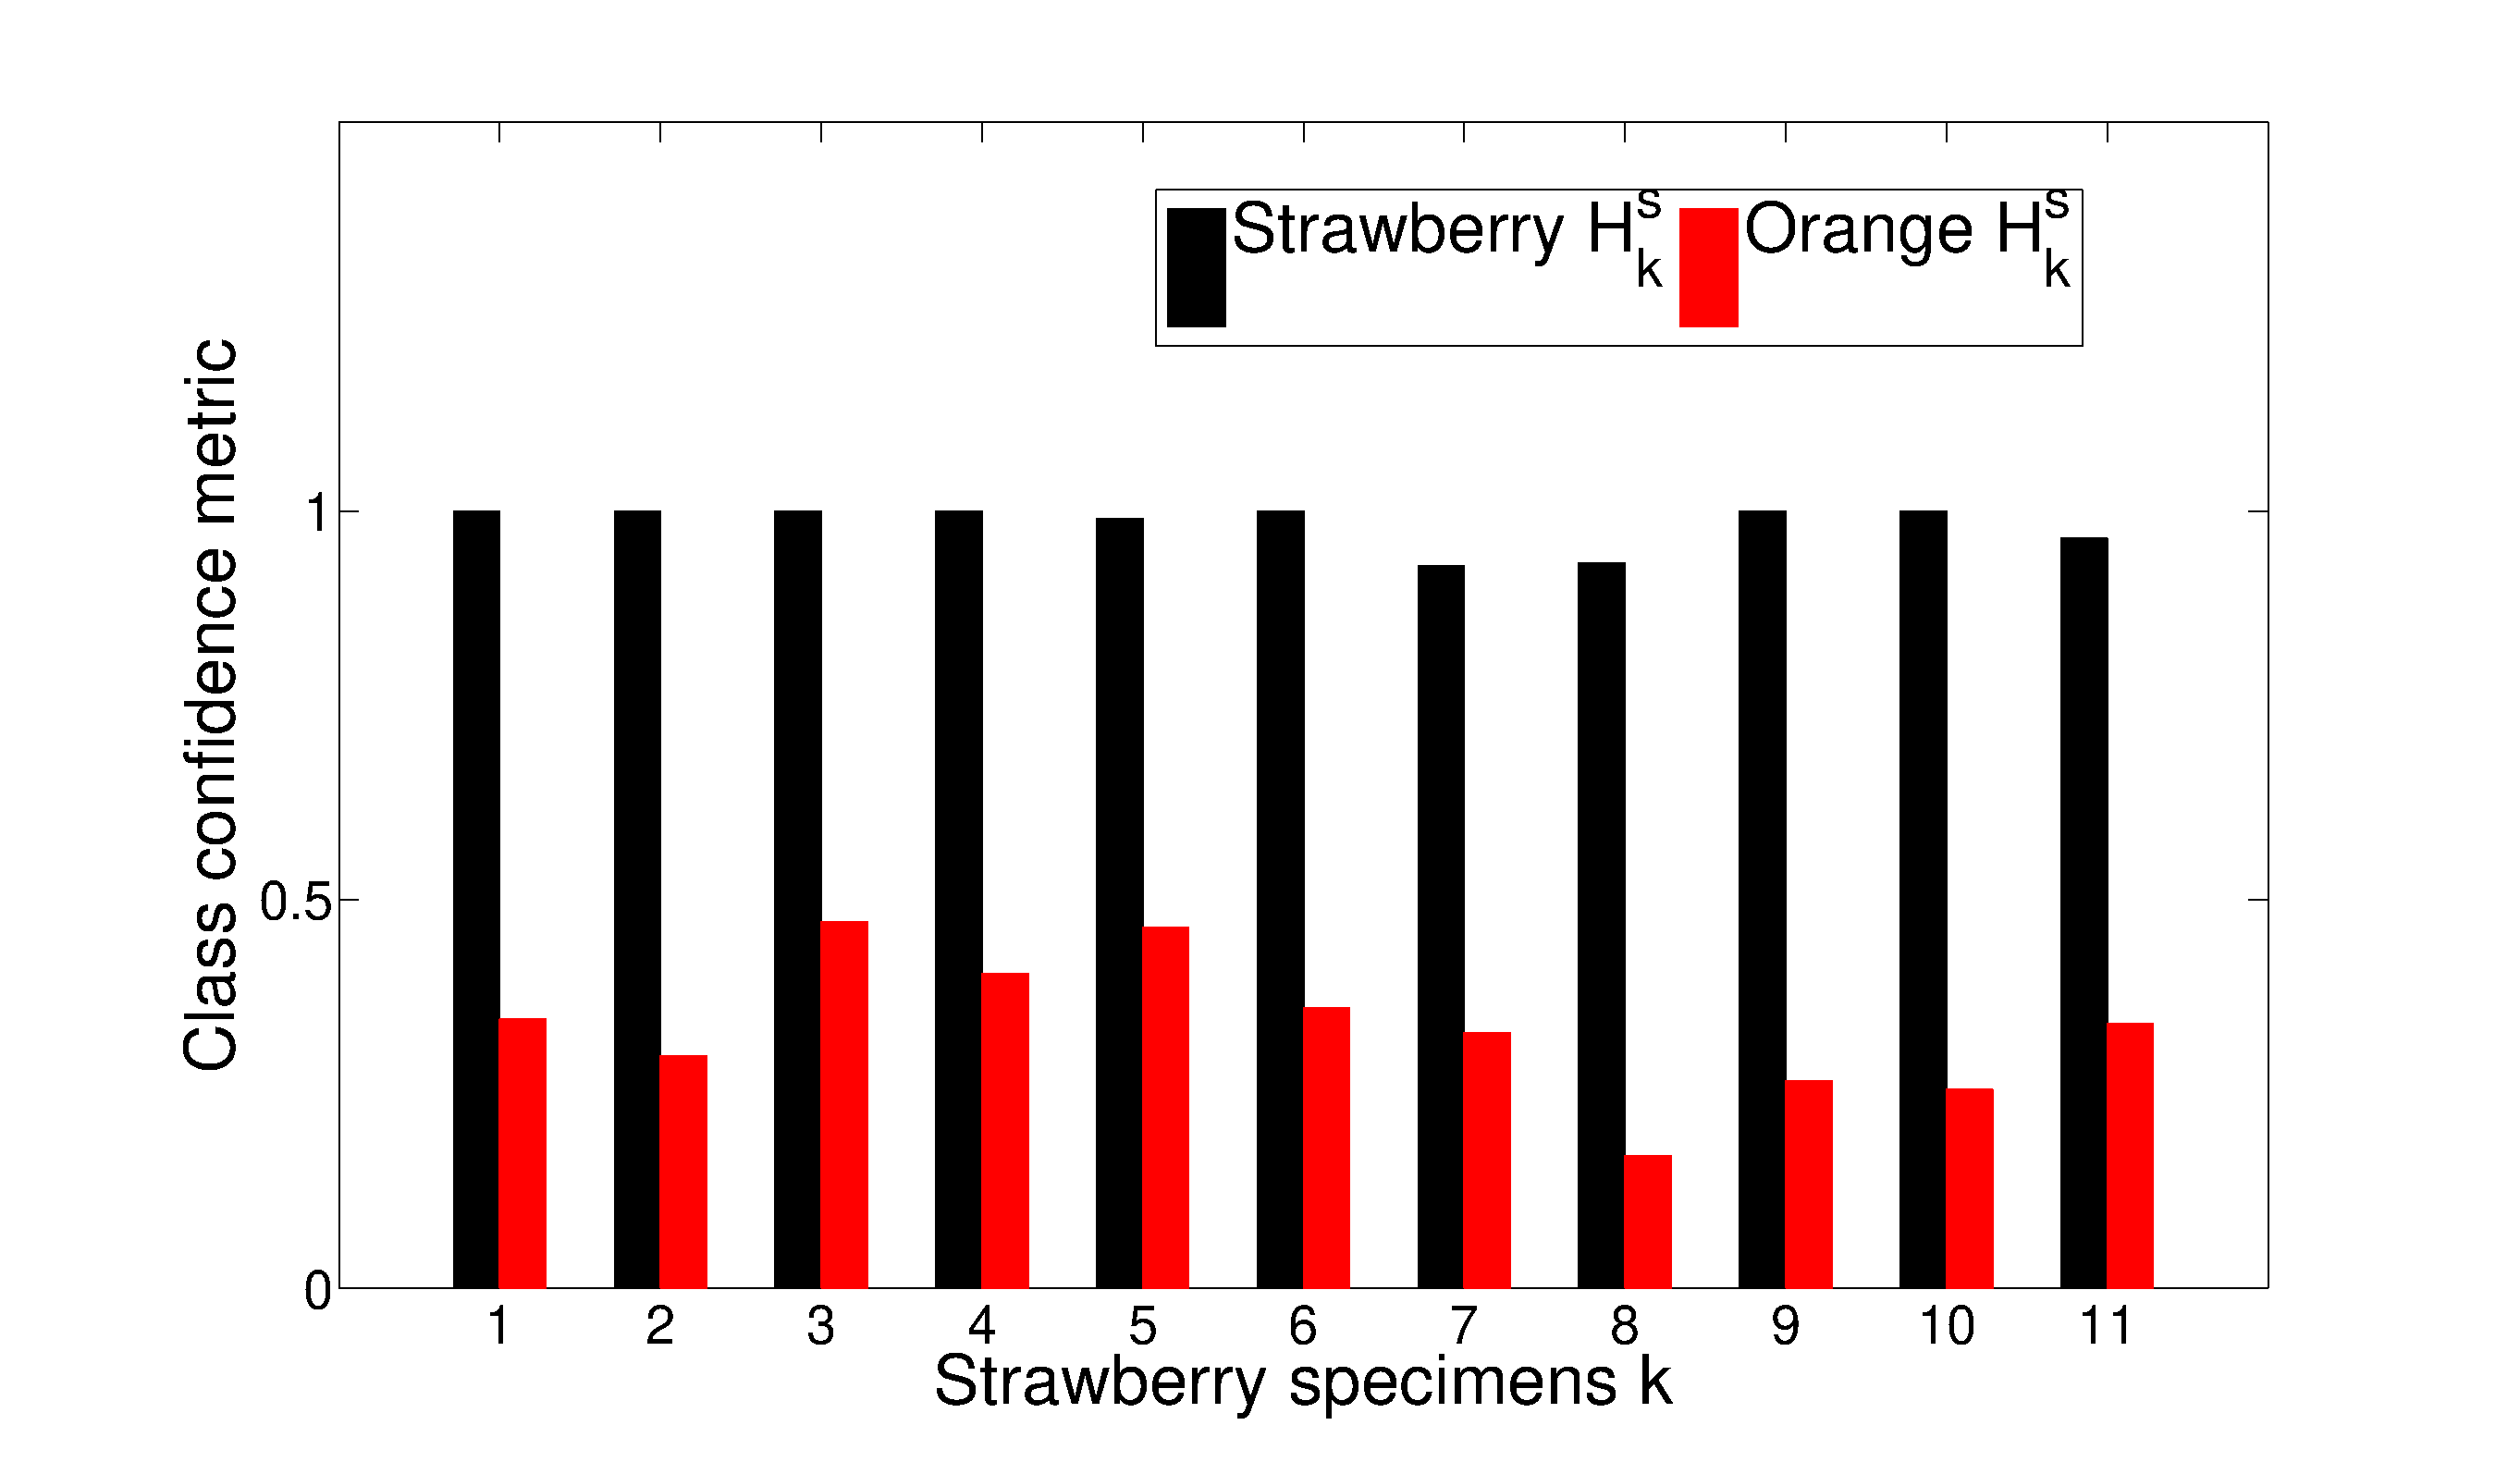
\includegraphics[width=\textwidth]{classification_metric_strawberry}
      \caption{}
      \label{fig:results_strawberry}
  \end{subfigure}
  \vskip -2pt
  \begin{subfigure}[]{0.7\textwidth}
      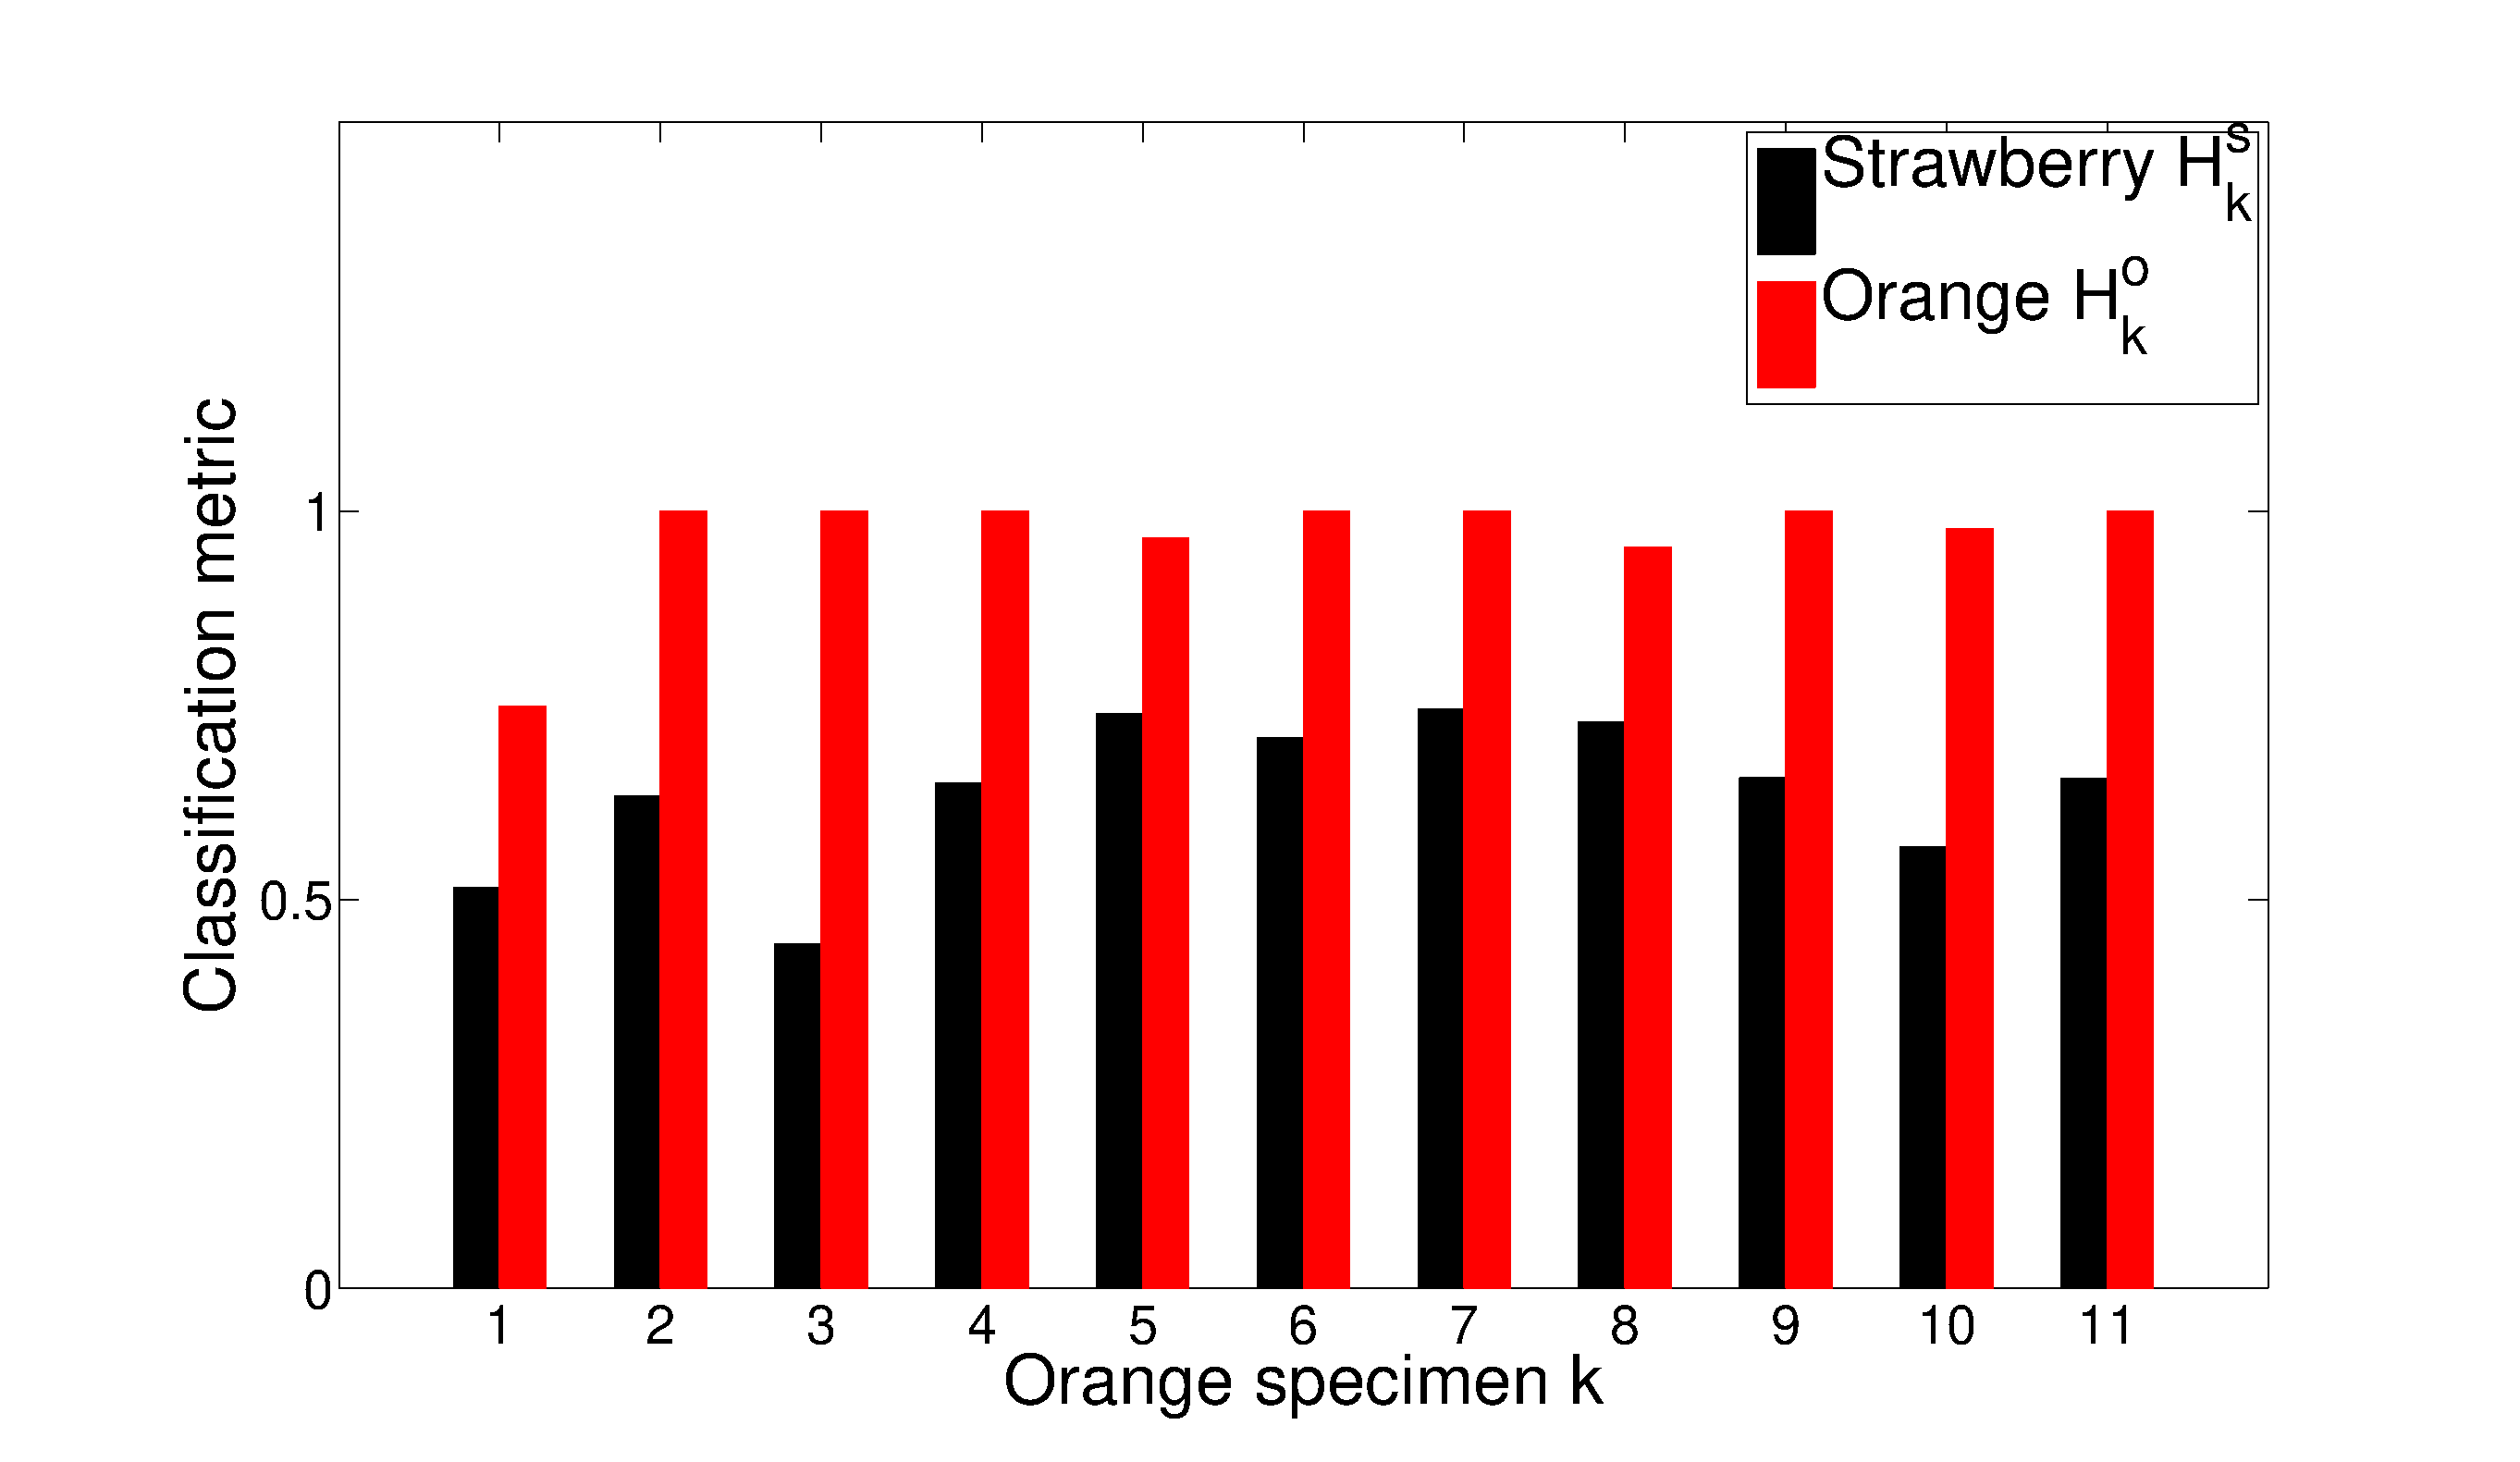
\includegraphics[width=\textwidth]{classification_metric_orange}
      \caption{}
      \label{fig:results_orange}
  \end{subfigure}
\caption[Classification results]{The classification results for the 11 strawberry and 11 orange specimens are shown in (\subref{fig:results_strawberry}) and (\subref{fig:results_orange}) respectively. The class confidence values $H^s_k$ and $H^o_k$ are shown by black and red bars. In the case of strawberry specimens in (\subref{fig:results_strawberry}), the black bars are taller than the red bars indicating that all strawberry specimens are classified correctly based on the hypothesis test of \eqref{eqn:binary_classification}. Same can be said in case of orange specimens shown in (\subref{fig:results_orange}) where the red bars are taller, indicating that all orange specimens are classified correctly.}
\label{fig:results}
\end{figure*}	
%

This validation procedure confirms the ability of this machine learning technique to combine data from multiple images of a specimen to perform a binary classification task. The 22 specimens drawn from strawberry and orange classes were all correctly classified by the proposed machine learning algorithm.

%================================================================================================================
\section{Discussion}
\begin{enumerate}
	\item The plots of the feature descriptor clearly show their conformance only to the feature distribution of the target class they belong to.
	
	\item Though capturing multiple images of a target object from different height could slowdown the imaging process and impose additional constrains on the object recognition process, detecting critical targets from noisy images justifies this end.
\end{enumerate}

The machine learning approach developed here was used to perform binary classification on a set of 22 specimens containing equal number of strawberry and orange specimens. The graphical results from Figures~\ref{fig:feat_results_strawberry_test} and \ref{fig:feat_results_orange_test} show the conformance of the distance measures $D^s_k$ and $D^o_k$ of different specimens, only to the respective class they belong to. This is further reinforced by the class confidence measures $H^s_k$ and $H^o_k$, which assigned each specimen to the right class. All the specimens were thus classified correctly, hence achieving 100\% precision and recall rates.\footnote{\emph{Precision} and \emph{Recall} are performance measures for a machine learning algorithm. Precision is the ratio of true positives to the total number of detections and recall is the ratio of true positives to the total number of positives in the dataset.} 

The theoretical best possible performance obtained here portrays the potential of this algorithm to work in noisy natural images. One source of noise in the data collection process has been a collection of floating specks of dust in the water, along with dust on the floor of the tank. There were even instances when the foot of the person operating the imaging-rig was included in the images collected. In addition, the uncontrolled lighting conditions introduced noise in the form of light artifacts in the floor of the tank. The effect of uneven lighting conditions under which the data collection process took place is visible in Figure~\ref{fig:height_specimen}. The ability of this algorithm to produce consistent high performance even in the presence of noise is evidence of its ability to handle unpredictable environmental conditions.

Since only 22 objects were used for this particular evaluation, testing this algorithm on a natural image dataset containing a few thousand specimens would definitively be interesting. Obtaining multiple images of the same specimen from different heights and annotating large learning sets, might appear cumbersome at first. However the semi-automated annotation procedure provided in Section~\ref{sec:distdes_annotation} alleviates considerably the manual labor involved.

Since this approach relies on multiple images for each specimen, imaging time and effort involved is typically higher than an object recognition algorithm that is designed to operate on a single image of a specimen. On the other hand, the use of multiple images and 39 independent hypothesis tests, contribute to identification of a target specimen with higher confidence than by an approach that just uses a single image of a target. Multiple images offer a way to extract features of an object from different scales, which when combined together offer a robust object recognition framework. In cases where it is critical to classify a target with confidence, for instance in case of detecting unexploded mines or submerged ordinance, an approach that is so accurate is  valuable despite the additional imaging time required.

%================================================================================================================
\section{Conclusion}
\begin{enumerate}
        \item The developed technique offers a way to detect objects from noisy images without any segmentation using images of a target captures from different height.
\end{enumerate}

The machine learning method developed here offers a way to perform binary classification using global descriptors generated from multiple images of a specimen. This technique was successful in recognizing all the 22 specimens available in our dataset of 11 strawberries and 11 oranges. The performance of this technique on this (admittedly small) dataset is the absolute theoretical maximum that can be obtained for a machine learning technique. This exceptional performance, despite the presence of noise and several uncontrolled variables in the data collection process, is indicative of the robustness of this algorithm. Additionally, the ability of this algorithm to perform object recognition via histogram based global descriptors, avoids segmentation entirely during the testing phase. Since segmentation can be problematic in noisy images where the edges of objects is hard to determine, doing away with segmentation is a great incentive to adopt this technique for noisy images.
%================================================================================================================
\section{Future work}

This algorithm has been tested on a set of 22 images collected using an imaging rig. It will be interesting to expand this technique to natural datasets where multiple instances of the same target object have been captured. The current procedure adopted here computes a set of discrete measurements from a fixed set of heights from which images are available. Expanding this to work with an arbitrary but known set of heights will be valuable for object recognition tasks where the data collected cannot adhere to such predetermined height standards. Expanding this binary classification problem into a multi-class classification problem for a larger number of object classes is another natural direction that can be explored.

%================================================================================================================

\printglossary[type=\acronymtype]                  
%
% This is the Bibliography file (bibtex.tex)
% This generally works for BibTeX

% Use sample.bib for BibTeX database
\bibliography{thesis_ref}
% BibTeX style (plain, alpha, unsrt)
\bibliographystyle{plain}
   % This file (bibtex.tex) contains the text
                   % for a bibliography if using BibTeX with
                   % sample.bib
\end{document}


